\documentclass[12pt,twoside]{report}

% =============================================================
% CONFIGURACIÓN GENERAL
% =============================================================

% Condicionales para configuración por modalidad
\usepackage{etoolbox}

% Datos generales y modalidad del proyecto
% =============================================================
% DATOS GENERALES DEL TRABAJO DE GRADO
% Edite este archivo para personalizar la portada, el encabezado
% y la modalidad del proyecto.
% =============================================================

% -------------------------------------------------------------
% Información general
% -------------------------------------------------------------

\newcommand{\ThesisTitle}{Conteo de rocas visibles basado en las máscaras de AI4Mars}
\newcommand{\ThesisShortTitle}{Conteo de rocas visibles en AI4Mars}
\newcommand{\ThesisAuthors}{Juan Pablo Delgado Castro}

\newcommand{\ThesisProgram}{Programa de Ciencia de Datos}
\newcommand{\ThesisDepartment}{Departamento de Matemáticas}
\newcommand{\ThesisUniversity}{Universidad Externado de Colombia}

\newcommand{\ThesisAdvisors}{Por completar}
\newcommand{\ThesisCity}{Bogotá, Colombia}
\newcommand{\ThesisYear}{2026}

% Archivo del logo institucional dentro de images/.
\newcommand{\UniversityLogo}{logo-externado-matematicas.png}


% =============================================================
% MODALIDAD DEL PROYECTO
% =============================================================

% Seleccione UNA de las siguientes modalidades:
%
% investigacion   = Investigación
% innovacion      = Innovación
% emprendimiento = Emprendimiento
%
% Solo debe modificar el valor de la siguiente línea.

\newcommand{\ModalidadProyecto}{investigacion}


% -------------------------------------------------------------
% Nombre de la modalidad para portada y otros elementos
% -------------------------------------------------------------

\ifdefstring{\ModalidadProyecto}{investigacion}{
  \newcommand{\TipoProyecto}{Informe de investigación}
}{
  \ifdefstring{\ModalidadProyecto}{innovacion}{
    \newcommand{\TipoProyecto}{Innovación}
  }{
    \ifdefstring{\ModalidadProyecto}{emprendimiento}{
      \newcommand{\TipoProyecto}{Emprendimiento}
    }{
      \newcommand{\TipoProyecto}{Modalidad no válida}
    }
  }
}


% -------------------------------------------------------------
% Compatibilidad con versiones anteriores de la plantilla
% -------------------------------------------------------------

% Mantiene funcionando archivos que todavía utilicen
% el comando \ProjectType.

\newcommand{\ProjectType}{\TipoProyecto}


% Cifras del documento, generadas a partir de los resultados con
% scripts/generar_cifras.py. No se escriben números a mano en el texto.
% =============================================================
% ARCHIVO GENERADO — no editar a mano.
% Generador: scripts/generar_cifras.py, a partir de outputs/.
% =============================================================

\newcommand{\cNEscenas}{\num{16064}}
\newcommand{\cNImagenes}{\num{18127}}
\newcommand{\cNCobCalc}{\num{15901}}
\newcommand{\cPctCobCalc}{\SI{99.0}{\percent}}
\newcommand{\cNCobPos}{\num{10817}}
\newcommand{\cPctCobPos}{\SI{67.3}{\percent}}
\newcommand{\cFracValidMed}{\num{0.58}}
\newcommand{\cFlagOk}{\num{2193}}
\newcommand{\cFlagOkPct}{\num{13.7}}
\newcommand{\cFlagNoBig}{\num{8458}}
\newcommand{\cFlagNoBigPct}{\num{52.7}}
\newcommand{\cFlagNoRock}{\num{4950}}
\newcommand{\cFlagNoRockPct}{\num{30.8}}
\newcommand{\cFlagNull}{\num{300}}
\newcommand{\cFlagNullPct}{\num{1.9}}
\newcommand{\cFlagEmpty}{\num{163}}
\newcommand{\cFlagEmptyPct}{\num{1.0}}
\newcommand{\cNBigAny}{\num{2226}}
\newcommand{\cPctBigAny}{\SI{13.9}{\percent}}
\newcommand{\cNNullBig}{\num{33}}
\newcommand{\cRocasNullBig}{\num{63}}
\newcommand{\cNOjoIzq}{\num{16027}}
\newcommand{\cNOjoDer}{\num{37}}
\newcommand{\cSecN}{\num{15601}}
\newcommand{\cSecTramos}{\num{40}}
\newcommand{\cSecPorTramo}{\num{390}}
\newcommand{\cSecMediaMax}{\SI{97.9}{\percent}}
\newcommand{\cSecMediaMin}{\SI{0.5}{\percent}}
\newcommand{\cSecBigMin}{\SI{0.3}{\percent}}
\newcommand{\cSecBigMax}{\SI{42.6}{\percent}}
\newcommand{\cSecTramosSuelo}{\num{15}}
\newcommand{\cSecTramosArena}{\num{0}}
\newcommand{\cCobMedVal}{\SI{96.8}{\percent}}
\newcommand{\cCobMediaVal}{\SI{75.1}{\percent}}
\newcommand{\cCobMedTot}{\SI{42.0}{\percent}}
\newcommand{\cCobMediaTot}{\SI{41.9}{\percent}}
\newcommand{\cNCobCien}{\num{4471}}
\newcommand{\cPctCobCien}{\SI{41.3}{\percent}}
\newcommand{\cNCobMitad}{\num{8339}}
\newcommand{\cNCobCero}{\num{5084}}
\newcommand{\cNRocas}{\num{4142}}
\newcommand{\cRocasMax}{\num{20}}
\newcommand{\cRocasMed}{\num{1}}
\newcommand{\cRawMedio}{\num{2.25}}
\newcommand{\cRocasMedio}{\num{1.89}}
\newcommand{\cBandaCero}{\num{452}}
\newcommand{\cBandaCeroPct}{\num{20.6}}
\newcommand{\cBandaUna}{\num{773}}
\newcommand{\cBandaUnaPct}{\num{35.2}}
\newcommand{\cBandaDosTres}{\num{613}}
\newcommand{\cBandaDosTresPct}{\num{28.0}}
\newcommand{\cBandaCuatroNueve}{\num{344}}
\newcommand{\cBandaCuatroNuevePct}{\num{15.7}}
\newcommand{\cBandaDiez}{\num{11}}
\newcommand{\cBandaDiezPct}{\num{0.5}}
\newcommand{\cTamPeq}{\num{1806}}
\newcommand{\cTamPeqPct}{\num{43.6}}
\newcommand{\cTamMed}{\num{1317}}
\newcommand{\cTamMedPct}{\num{31.8}}
\newcommand{\cTamGra}{\num{1019}}
\newcommand{\cTamGraPct}{\num{24.6}}
\newcommand{\cNConRocas}{\num{1741}}
\newcommand{\cSolidezMedia}{\num{0.912}}
\newcommand{\cNSolidezBaja}{\num{44}}
\newcommand{\cNSubdiv}{\num{417}}
\newcommand{\cPctSubdiv}{\SI{24.0}{\percent}}
\newcommand{\cRocasSubdiv}{\num{1692}}
\newcommand{\cNMayorMitad}{\num{32}}
\newcommand{\cCompBed}{\SI{49.8}{\percent}}
\newcommand{\cCompSoil}{\SI{36.4}{\percent}}
\newcommand{\cCompSand}{\SI{12.5}{\percent}}
\newcommand{\cCompBig}{\SI{1.3}{\percent}}
\newcommand{\cDomBed}{\num{8234}}
\newcommand{\cDomSoil}{\num{5767}}
\newcommand{\cDomSand}{\num{1792}}
\newcommand{\cDomBig}{\num{108}}
\newcommand{\cTipoRocoso}{\num{7601}}
\newcommand{\cTipoRocosoPct}{\num{47.3}}
\newcommand{\cTipoSuelo}{\num{5723}}
\newcommand{\cTipoSueloPct}{\num{35.6}}
\newcommand{\cTipoArenoso}{\num{1742}}
\newcommand{\cTipoArenosoPct}{\num{10.8}}
\newcommand{\cTipoMixto}{\num{835}}
\newcommand{\cTipoMixtoPct}{\num{5.2}}
\newcommand{\cTipoSinEtiq}{\num{163}}
\newcommand{\cTipoSinEtiqPct}{\num{1.0}}
\newcommand{\cNSinBig}{\num{13838}}
\newcommand{\cPctSinBig}{\SI{86.1}{\percent}}
\newcommand{\cNoBigBedMed}{\SI{99.7}{\percent}}
\newcommand{\cNoBigBedOchenta}{\num{5762}}
\newcommand{\cParteBed}{\SI{97.5}{\percent}}
\newcommand{\cParteBig}{\SI{2.5}{\percent}}
\newcommand{\cNFiltradas}{\num{452}}
\newcommand{\cPctFiltradas}{\SI{2.8}{\percent}}
\newcommand{\cPctNullBig}{\SI{0.2}{\percent}}
\newcommand{\cPctConRocas}{\SI{10.8}{\percent}}
\newcommand{\cNArtefacto}{\num{3}}
\newcommand{\cNArtefactoOk}{\num{0}}
\newcommand{\cSensRho}{\num{0.90}}
\newcommand{\cSensRhoRoca}{\num{0.68}}
\newcommand{\cSensMitadTot}{\num{4387}}
\newcommand{\cSensConteoPearson}{\num{-0.027}}
\newcommand{\cSensConteoPearsonP}{\num{0.201}}
\newcommand{\cSensConteoSpearman}{\ensuremath{+}\num{0.015}}
\newcommand{\cSensConteoSpearmanP}{\num{0.478}}
\newcommand{\cSensTotColab}{\SI{42.0}{\percent}}
\newcommand{\cSensTotExp}{\SI{19.8}{\percent}}
\newcommand{\cSensTotP}{< \num{0.001}}
\newcommand{\cGoldUnoBig}{\SI{16.5}{\percent}}
\newcommand{\cGoldUnoRocas}{\num{0.29}}
\newcommand{\cGoldUnoCobMed}{\SI{12.5}{\percent}}
\newcommand{\cNGold}{\num{322}}
\newcommand{\cGoldCobMedPos}{\SI{46.1}{\percent}}
\newcommand{\cGoldSueloArena}{\SI{67.1}{\percent}}
\newcommand{\cGoldBed}{\SI{32.7}{\percent}}
\newcommand{\cGoldPctCien}{\SI{8}{\percent}}
\newcommand{\cGoldDosBig}{\SI{6.2}{\percent}}
\newcommand{\cGoldDosRocas}{\num{0.10}}
\newcommand{\cGoldDosCobMed}{\SI{7.7}{\percent}}
\newcommand{\cGoldTresBig}{\SI{1.6}{\percent}}
\newcommand{\cGoldTresRocas}{\num{0.03}}
\newcommand{\cGoldTresCobMed}{\SI{0.8}{\percent}}
\newcommand{\cColabCobMed}{\SI{58.6}{\percent}}
\newcommand{\cColabRocas}{\num{0.26}}
\newcommand{\cColabSueloArena}{\SI{48.9}{\percent}}
\newcommand{\cColabBed}{\SI{49.8}{\percent}}
\newcommand{\cColabPctCien}{\SI{41}{\percent}}
\newcommand{\cFANColab}{\num{593}}
\newcommand{\cFANExp}{\num{322}}
\newcommand{\cFAEtiqMedColab}{\SI{66.9}{\percent}}
\newcommand{\cFAEtiqMedExp}{\SI{12.5}{\percent}}
\newcommand{\cFAEtiqMediaColab}{\SI{53.3}{\percent}}
\newcommand{\cFAEtiqMediaExp}{\SI{32.9}{\percent}}
\newcommand{\cFAEtiqP}{< \num{0.001}}
\newcommand{\cFARegMedColab}{\SI{72.5}{\percent}}
\newcommand{\cFARegMedExp}{\SI{5.8}{\percent}}
\newcommand{\cFARegMediaColab}{\SI{54.4}{\percent}}
\newcommand{\cFARegMediaExp}{\SI{36.1}{\percent}}
\newcommand{\cFARegP}{< \num{0.001}}
\newcommand{\cFAValMedColab}{\SI{74.3}{\percent}}
\newcommand{\cFAValMedExp}{\SI{6.1}{\percent}}
\newcommand{\cFAValMediaColab}{\SI{54.3}{\percent}}
\newcommand{\cFAValMediaExp}{\SI{36.0}{\percent}}
\newcommand{\cFAValP}{< \num{0.001}}
\newcommand{\cFAFracColab}{\num{0.89}}
\newcommand{\cFAFracExp}{\num{0.92}}
\newcommand{\cDescTotal}{\ensuremath{+}\num{20.4}}
\newcommand{\cDescImg}{\ensuremath{+}\num{18.2}}
\newcommand{\cDescAnot}{\ensuremath{+}\num{2.2}}
\newcommand{\cDescImgPct}{\SI{89}{\percent}}
\newcommand{\cDescAnotPct}{\SI{11}{\percent}}
\newcommand{\cDescImgIC}{[\ensuremath{+}\num{12.4}; \ensuremath{+}\num{23.8}]}
\newcommand{\cDescAnotIC}{[\ensuremath{+}\num{0.02}; \ensuremath{+}\num{4.54}]}
\newcommand{\cResColab}{\num{-1.0}}
\newcommand{\cResExp}{\num{-3.2}}
\newcommand{\cFuenteDifMed}{\ensuremath{+}\num{50.7}}
\newcommand{\cFuenteDifIC}{[\ensuremath{+}\num{36.0}; \ensuremath{+}\num{64.7}]}
\newcommand{\cFuenteMWp}{< \num{0.001}}
\newcommand{\cFracValidGold}{\num{0.59}}
\newcommand{\cFracValidP}{\num{0.24}}
\newcommand{\cDepCCN}{\num{2193}}
\newcommand{\cDepCCPearson}{\ensuremath{+}\num{0.022}}
\newcommand{\cDepCCPearsonIC}{[\num{-0.015}; \ensuremath{+}\num{0.060}]}
\newcommand{\cDepCCPearsonP}{= \num{0.286}}
\newcommand{\cDepCCSpearman}{\ensuremath{+}\num{0.020}}
\newcommand{\cDepCCSpearmanIC}{[\num{-0.021}; \ensuremath{+}\num{0.060}]}
\newcommand{\cDepCCSpearmanP}{= \num{0.351}}
\newcommand{\cDepCCKendall}{\ensuremath{+}\num{0.018}}
\newcommand{\cDepCCKendallP}{= \num{0.271}}
\newcommand{\cDepCCDcor}{\num{0.074}}
\newcommand{\cDepCCDcorP}{= \num{0.002}}
\newcommand{\cDepCCIM}{\num{0.123}}
\newcommand{\cDepCCIMNula}{\num{0.023}}
\newcommand{\cDepCCIMP}{\leq \num{0.005}}
\newcommand{\cDepFCN}{\num{15901}}
\newcommand{\cDepFCPearson}{\num{-0.020}}
\newcommand{\cDepFCPearsonIC}{[\num{-0.036}; \num{-0.004}]}
\newcommand{\cDepFCPearsonP}{= \num{0.011}}
\newcommand{\cDepFCSpearman}{\num{-0.021}}
\newcommand{\cDepFCSpearmanIC}{[\num{-0.037}; \num{-0.004}]}
\newcommand{\cDepFCSpearmanP}{= \num{0.012}}
\newcommand{\cDepFCKendall}{\num{-0.014}}
\newcommand{\cDepFCKendallP}{= \num{0.013}}
\newcommand{\cDepFCDcor}{\num{0.062}}
\newcommand{\cDepFCDcorP}{\leq \num{0.001}}
\newcommand{\cDepFCIM}{\num{0.037}}
\newcommand{\cDepFCIMNula}{\num{0.011}}
\newcommand{\cDepFCIMP}{\leq \num{0.005}}
\newcommand{\cDepFTN}{\num{15901}}
\newcommand{\cDepFTPearson}{\ensuremath{+}\num{0.362}}
\newcommand{\cDepFTPearsonIC}{[\ensuremath{+}\num{0.349}; \ensuremath{+}\num{0.375}]}
\newcommand{\cDepFTPearsonP}{\leq \num{0.001}}
\newcommand{\cDepFTSpearman}{\ensuremath{+}\num{0.235}}
\newcommand{\cDepFTSpearmanIC}{[\ensuremath{+}\num{0.218}; \ensuremath{+}\num{0.250}]}
\newcommand{\cDepFTSpearmanP}{\leq \num{0.001}}
\newcommand{\cDepFTKendall}{\ensuremath{+}\num{0.230}}
\newcommand{\cDepFTKendallP}{\leq \num{0.001}}
\newcommand{\cDepFTDcor}{\num{0.409}}
\newcommand{\cDepFTDcorP}{\leq \num{0.001}}
\newcommand{\cDepFTIM}{\num{2.766}}
\newcommand{\cDepFTIMNula}{\num{0.010}}
\newcommand{\cDepFTIMP}{\leq \num{0.005}}
\newcommand{\cChiDos}{\num{23.7}}
\newcommand{\cChiGl}{\num{12}}
\newcommand{\cChiP}{\num{0.022}}
\newcommand{\cCramer}{\num{0.060}}
\newcommand{\cDepDcorSub}{\num{3000}}
\newcommand{\cEtaConteo}{\SI{5.6}{\percent}}
\newcommand{\cEtaGrupos}{\num{8}}
\newcommand{\cEtaCob}{\SI{0.3}{\percent}}
\newcommand{\cEtaConteoNula}{\SI{0.7}{\percent}}
\newcommand{\cEtaConteoP}{\leq \num{0.001}}
\newcommand{\cEtaCobNula}{\SI{0.4}{\percent}}
\newcommand{\cEtaCobP}{= \num{0.133}}
\newcommand{\cUNA}{\num{443}}
\newcommand{\cUMediaA}{\num{1.40}}
\newcommand{\cUCeroA}{\num{23.0}}
\newcommand{\cUCuatroA}{\num{7.2}}
\newcommand{\cUNB}{\num{384}}
\newcommand{\cUMediaB}{\num{2.40}}
\newcommand{\cUCeroB}{\num{16.1}}
\newcommand{\cUCuatroB}{\num{25.8}}
\newcommand{\cUNC}{\num{392}}
\newcommand{\cUMediaC}{\num{2.08}}
\newcommand{\cUCeroC}{\num{18.4}}
\newcommand{\cUCuatroC}{\num{19.9}}
\newcommand{\cUND}{\num{490}}
\newcommand{\cUMediaD}{\num{1.98}}
\newcommand{\cUCeroD}{\num{19.8}}
\newcommand{\cUCuatroD}{\num{17.6}}
\newcommand{\cUNE}{\num{484}}
\newcommand{\cUMediaE}{\num{1.68}}
\newcommand{\cUCeroE}{\num{24.6}}
\newcommand{\cUCuatroE}{\num{12.4}}
\newcommand{\cFTNA}{\num{1895}}
\newcommand{\cFTMedA}{\SI{48.2}{\percent}}
\newcommand{\cFTMedTotA}{\SI{3.4}{\percent}}
\newcommand{\cFTNB}{\num{4249}}
\newcommand{\cFTMedB}{\SI{59.2}{\percent}}
\newcommand{\cFTMedTotB}{\SI{22.0}{\percent}}
\newcommand{\cFTNC}{\num{5680}}
\newcommand{\cFTMedC}{\SI{69.3}{\percent}}
\newcommand{\cFTMedTotC}{\SI{42.8}{\percent}}
\newcommand{\cFTND}{\num{4077}}
\newcommand{\cFTMedD}{\SI{32.6}{\percent}}
\newcommand{\cFTMedTotD}{\SI{26.6}{\percent}}
\newcommand{\cFTCeroA}{\SI{32.6}{\percent}}
\newcommand{\cFTCienA}{\SI{28.1}{\percent}}
\newcommand{\cFTMedRocaA}{\SI{95.7}{\percent}}
\newcommand{\cFTCeroB}{\SI{29.3}{\percent}}
\newcommand{\cFTCienB}{\SI{24.8}{\percent}}
\newcommand{\cFTMedRocaB}{\SI{91.8}{\percent}}
\newcommand{\cFTCeroC}{\SI{27.3}{\percent}}
\newcommand{\cFTCienC}{\SI{28.0}{\percent}}
\newcommand{\cFTMedRocaC}{\SI{95.2}{\percent}}
\newcommand{\cFTCeroD}{\SI{41.0}{\percent}}
\newcommand{\cFTCienD}{\SI{31.7}{\percent}}
\newcommand{\cFTMedRocaD}{\SI{100.0}{\percent}}
\newcommand{\cVN}{\num{60}}
\newcommand{\cVAcuerdo}{\SI{50}{\percent}}
\newcommand{\cVSignoP}{< \num{0.001}}
\newcommand{\cVKappa}{\num{0.13}}
\newcommand{\cVKappaPond}{\num{0.11}}
\newcommand{\cVKappaIC}{[\ensuremath{+}\num{0.00}; \ensuremath{+}\num{0.27}]}
\newcommand{\cVKappaPondIC}{[\ensuremath{+}\num{0.01}; \ensuremath{+}\num{0.22}]}
\newcommand{\cVAbajo}{\num{28}}
\newcommand{\cVArriba}{\num{2}}
\newcommand{\cVMaxAuto}{\num{9}}
\newcommand{\cVHumDiez}{\num{12}}
\newcommand{\cVHumVeinti}{\num{5}}
\newcommand{\cVCoincUnaTres}{\num{26}}
\newcommand{\cVCoinc}{\num{30}}
\newcommand{\cVRocasAuto}{\num{133}}
\newcommand{\cVRocasHumMin}{\num{302}}
\newcommand{\cVRocasHumMax}{\num{674}}
\newcommand{\cVRazon}{\num{2.3}}
\newcommand{\cVDeficit}{\num{196}}
\newcommand{\cVNoExhN}{\num{36}}
\newcommand{\cVNoExhMed}{\SI{9.1}{\percent}}
\newcommand{\cVUnaTresN}{\num{27}}
\newcommand{\cVUnaTresZona}{\SI{1.11}{\percent}}
\newcommand{\cVUnaTresFr}{\SI{5.4}{\percent}}
\newcommand{\cSenN}{\num{36}}
\newcommand{\cSenMin}{\num{0.07}}
\newcommand{\cSenMax}{\num{0.21}}
\newcommand{\cSenMed}{\num{0.11}}
\newcommand{\cSenAbajo}{\num{36}}
\newcommand{\cSenAbajoMin}{\num{23}}
\newcommand{\cSenAbajoMax}{\num{29}}
\newcommand{\cSenArribaMax}{\num{5}}
\newcommand{\cSenDiez}{\num{5}}
\newcommand{\cMIGradKw}{\num{0.18}}
\newcommand{\cMIGradAbajo}{\num{9}}
\newcommand{\cMIGradArriba}{\num{24}}
\newcommand{\cMIGradDif}{\ensuremath{+}\num{0.06}}
\newcommand{\cMIGradIC}{[\num{-0.14}; \ensuremath{+}\num{0.28}]}
\newcommand{\cMIGradICB}{[\num{-0.19}; \ensuremath{+}\num{0.33}]}
\newcommand{\cMIPersistKw}{\num{0.08}}
\newcommand{\cMIPersistAbajo}{\num{9}}
\newcommand{\cMIPersistArriba}{\num{40}}
\newcommand{\cMIPersistDif}{\num{-0.03}}
\newcommand{\cMIPersistIC}{[\num{-0.20}; \ensuremath{+}\num{0.13}]}
\newcommand{\cMIPersistICB}{[\num{-0.24}; \ensuremath{+}\num{0.17}]}
\newcommand{\cMISombraKw}{\num{0.37}}
\newcommand{\cMISombraAbajo}{\num{10}}
\newcommand{\cMISombraArriba}{\num{19}}
\newcommand{\cMISombraDif}{\ensuremath{+}\num{0.26}}
\newcommand{\cMISombraIC}{[\ensuremath{+}\num{0.03}; \ensuremath{+}\num{0.47}]}
\newcommand{\cMISombraICB}{[\num{-0.03}; \ensuremath{+}\num{0.53}]}
\newcommand{\cMIComboKw}{\num{0.27}}
\newcommand{\cMIComboAbajo}{\num{7}}
\newcommand{\cMIComboArriba}{\num{26}}
\newcommand{\cMIComboDif}{\ensuremath{+}\num{0.15}}
\newcommand{\cMIComboIC}{[\num{-0.05}; \ensuremath{+}\num{0.36}]}
\newcommand{\cMIComboICB}{[\num{-0.11}; \ensuremath{+}\num{0.41}]}
\newcommand{\cMISombraVarN}{\num{15}}
\newcommand{\cMISombraVarMin}{\num{0.08}}
\newcommand{\cMISombraVarMax}{\num{0.37}}
\newcommand{\cMISombraVarBonf}{\num{0}}
\newcommand{\cSplitRocaTrain}{\SI{37.6}{\percent}}
\newcommand{\cSplitIgnTrain}{\SI{39.5}{\percent}}
\newcommand{\cSplitRocaVal}{\SI{36.0}{\percent}}
\newcommand{\cSplitIgnVal}{\SI{37.8}{\percent}}
\newcommand{\cSplitRocaTest}{\SI{42.8}{\percent}}
\newcommand{\cSplitIgnTest}{\SI{39.5}{\percent}}
\newcommand{\cSegTrain}{\num{2000}}
\newcommand{\cSegVal}{\num{400}}
\newcommand{\cSegTest}{\num{400}}
\newcommand{\cSegEpocas}{\num{6}}
\newcommand{\cSegLado}{\num{512}}
\newcommand{\cSegLote}{\num{4}}
\newcommand{\cSegLR}{\num{1e-4}}
\newcommand{\cSegCandidatas}{\num{15601}}
\newcommand{\cSegElegibles}{\num{14490}}
\newcommand{\cSegExcluidas}{\num{1111}}
\newcommand{\cSegMargen}{\num{187}}
\newcommand{\cSegSolesBloque}{\num{75}}
\newcommand{\cSegEpocaElegida}{\num{4}}
\newcommand{\cSegHash}{ea767438f90218d2…}
\newcommand{\cSegHashCompleto}{ea767438f90218d2dd58829b6a234e8a0e41f344f0552da96bf297036934a104}
\newcommand{\cSegMinEpocaMin}{\num{12}}
\newcommand{\cSegMinEpocaMax}{\num{23}}
\newcommand{\cSegMinTotal}{\num{99}}
\newcommand{\cSegValMIoU}{\num{0.957}}
\newcommand{\cSegValUltima}{\num{0.948}}
\newcommand{\cSegIoUNo}{\num{0.947}}
\newcommand{\cSegIoURoca}{\num{0.932}}
\newcommand{\cSegMIoU}{\num{0.940}}
\newcommand{\cSegRCob}{\num{0.971}}
\newcommand{\cSegMAE}{\num{3.5}}
\newcommand{\cSegErrMedio}{\ensuremath{+}\num{0.9}}
\newcommand{\cSegDistMin}{\num{1.0}}
\newcommand{\cSegDistMed}{\num{30}}
\newcommand{\cSegNatN}{\num{2323}}
\newcommand{\cSegNatMIoU}{\num{0.932}}
\newcommand{\cSegNatR}{\num{0.971}}
\newcommand{\cSegNatMAE}{\num{3.7}}
\newcommand{\cSegNatErr}{\ensuremath{+}\num{0.9}}
\newcommand{\cSegNatIoURoca}{\num{0.949}}
\newcommand{\cSegNatIoUNo}{\num{0.914}}
\newcommand{\cSegExcN}{\num{178}}
\newcommand{\cSegExcMIoU}{\num{0.815}}
\newcommand{\cSegExcR}{\num{0.869}}
\newcommand{\cSegExcMAE}{\num{10.4}}
\newcommand{\cSegExcErr}{\num{-0.7}}
\newcommand{\cSegExcIoURoca}{\num{0.828}}
\newcommand{\cSegExcIoUNo}{\num{0.802}}
\newcommand{\cAleMIoU}{\num{0.940}}
\newcommand{\cAleR}{\num{0.971}}
\newcommand{\cAleMAE}{\num{3.0}}
\newcommand{\cAleMinuto}{\num{75}}
\newcommand{\cAleMinutoPct}{\SI{19}{\percent}}
\newcommand{\cFugaMinSoles}{\num{1.1}}
\newcommand{\cFugaMedGapSoles}{\num{31}}
\newcommand{\cFugaNA}{\num{94}}
\newcommand{\cFugaIoUA}{\num{0.939}}
\newcommand{\cFugaRA}{\num{0.969}}
\newcommand{\cFugaMAEA}{\num{2.9}}
\newcommand{\cFugaErrA}{\num{-0.02}}
\newcommand{\cFugaNB}{\num{212}}
\newcommand{\cFugaIoUB}{\num{0.945}}
\newcommand{\cFugaRB}{\num{0.969}}
\newcommand{\cFugaMAEB}{\num{3.3}}
\newcommand{\cFugaErrB}{\ensuremath{+}\num{0.65}}
\newcommand{\cFugaNC}{\num{94}}
\newcommand{\cFugaIoUC}{\num{0.925}}
\newcommand{\cFugaRC}{\num{0.977}}
\newcommand{\cFugaMAEC}{\num{4.2}}
\newcommand{\cFugaErrC}{\ensuremath{+}\num{2.47}}
\newcommand{\cFugaExpSol}{\num{67}}
\newcommand{\cFugaExpHora}{\num{0}}
\newcommand{\cFugaExpSoles}{\num{3.1}}
\newcommand{\cExpIoUNo}{\num{0.889}}
\newcommand{\cExpIoURoca}{\num{0.783}}
\newcommand{\cExpMIoU}{\num{0.836}}
\newcommand{\cExpR}{\num{0.924}}
\newcommand{\cExpExactas}{\SI{32}{\percent}}
\newcommand{\cExpExactasCero}{\SI{89}{\percent}}
\newcommand{\cBAColN}{\num{593}}
\newcommand{\cBAColMedia}{\ensuremath{+}\num{0.93}}
\newcommand{\cBAColMediaIC}{[\num{-0.08}; \ensuremath{+}\num{1.90}]}
\newcommand{\cBAColMediana}{\ensuremath{+}\num{0.0}}
\newcommand{\cBAColMAE}{\num{4.3}}
\newcommand{\cBAColMAEIC}{[\num{3.4}; \num{5.3}]}
\newcommand{\cBAColLoA}{[\num{-23.3}; \ensuremath{+}\num{25.2}]}
\newcommand{\cBAColDiez}{\SI{11.1}{\percent}}
\newcommand{\cBAColCincuenta}{\SI{1.5}{\percent}}
\newcommand{\cBAColPct}{[\num{-14.9}; \ensuremath{+}\num{24.5}]}
\newcommand{\cBAColEncima}{\SI{30.4}{\percent}}
\newcommand{\cBAColDebajo}{\SI{21.8}{\percent}}
\newcommand{\cBAExpN}{\num{322}}
\newcommand{\cBAExpMedia}{\ensuremath{+}\num{3.12}}
\newcommand{\cBAExpMediaIC}{[\ensuremath{+}\num{1.36}; \ensuremath{+}\num{4.95}]}
\newcommand{\cBAExpMediana}{\ensuremath{+}\num{0.0}}
\newcommand{\cBAExpMAE}{\num{8.5}}
\newcommand{\cBAExpMAEIC}{[\num{7.1}; \num{10.2}]}
\newcommand{\cBAExpLoA}{[\num{-29.3}; \ensuremath{+}\num{35.6}]}
\newcommand{\cBAExpDiez}{\SI{28.0}{\percent}}
\newcommand{\cBAExpCincuenta}{\SI{2.2}{\percent}}
\newcommand{\cBAExpPct}{[\num{-24.6}; \ensuremath{+}\num{37.8}]}
\newcommand{\cBAExpEncima}{\SI{42.5}{\percent}}
\newcommand{\cBAExpDebajo}{\SI{25.2}{\percent}}
\newcommand{\cSamN}{\num{50}}
\newcommand{\cSamAcuerdo}{\SI{52}{\percent}}
\newcommand{\cSamRho}{\num{0.45}}
\newcommand{\cSamMAE}{\num{2.6}}
\newcommand{\cCalRedBaja}{\SI{21}{\percent}}
\newcommand{\cCalNBaja}{\num{20}}
\newcommand{\cCalRedMuchas}{\SI{41}{\percent}}
\newcommand{\cCalNMuchas}{\num{6}}
\newcommand{\cCalNormN}{\num{2167}}
\newcommand{\cCalNormSinCambio}{\num{1519}}
\newcommand{\cCalRedNorm}{\SI{21}{\percent}}
\newcommand{\cCalSemillasA}{\num{142}}
\newcommand{\cPruebasN}{\num{10}}
\newcommand{\cHibridoN}{\num{351}}
\newcommand{\cHibridoRegion}{\SI{98.8}{\percent}}
\newcommand{\cFPNColab}{\num{600}}
\newcommand{\cFPDescImg}{\ensuremath{+}\num{27.0}}
\newcommand{\cFPDescAnot}{\ensuremath{+}\num{3.2}}
\newcommand{\cFPDescImgPct}{\SI{89}{\percent}}
\newcommand{\cFPDescAnotIC}{[\ensuremath{+}\num{1.0}; \ensuremath{+}\num{5.4}]}
\newcommand{\cFPRegMedColab}{\SI{94.3}{\percent}}
\newcommand{\cFVDescImgPct}{\SI{76}{\percent}}
\newcommand{\cFVDescAnot}{\ensuremath{+}\num{4.4}}
\newcommand{\cFVDescAnotIC}{[\ensuremath{+}\num{2.1}; \ensuremath{+}\num{6.5}]}
\newcommand{\cGeoN}{\num{8497}}
\newcommand{\cGeoVeta}{\num{294}}
\newcommand{\cGeoVetaPct}{\SI{3.5}{\percent}}
\newcommand{\cGeoVetaProb}{\num{150}}
\newcommand{\cGeoVetaDud}{\num{69}}
\newcommand{\cGeoVetaResto}{\num{75}}
\newcommand{\cGeoFloatPct}{\SI{61.2}{\percent}}
\newcommand{\cConsBig}{\SI{20}{\percent}}
\newcommand{\cConsBed}{\SI{44}{\percent}}
\newcommand{\cConsSoil}{\SI{67}{\percent}}
\newcommand{\cConsSand}{\SI{68}{\percent}}
\newcommand{\cTempNSolesEUno}{\num{1441}}
\newcommand{\cTempEscSolEUno}{\num{8}}
\newcommand{\cTempFCIC}{[\num{-0.047}; \num{0.008}]}
\newcommand{\cTempFCP}{= \num{0.623}}
\newcommand{\cTempNSolesEDos}{\num{576}}
\newcommand{\cTempCCIC}{[\num{-0.019}; \num{0.064}]}
\newcommand{\cTempCCP}{= \num{0.478}}
\newcommand{\cTempDcorP}{= \num{0.026}}
\newcommand{\cTempEtaP}{\leq \num{0.001}}
\newcommand{\cTempNSolesExp}{\num{48}}
\newcommand{\cTempAnotIC}{[\num{-1.0}; \ensuremath{+}\num{5.5}]}
\newcommand{\cTempBAIC}{[\ensuremath{+}\num{0.53}; \ensuremath{+}\num{5.98}]}
\newcommand{\cTempAnotPruebaIC}{[\ensuremath{+}\num{0.2}; \ensuremath{+}\num{6.3}]}
\newcommand{\cPrioAlta}{\num{98}}
\newcommand{\cPrioMedia}{\num{1343}}
\newcommand{\cPrioBaja}{\num{124}}
\newcommand{\cPrioSin}{\num{14499}}
\newcommand{\cReglaRocoso}{\num{6855}}
\newcommand{\cReglaArena}{\num{1174}}
\newcommand{\cReglaNoEval}{\num{463}}
\newcommand{\cReglaMayor}{\num{233}}
\newcommand{\cReglaCampo}{\num{195}}
\newcommand{\cReglaAngulosos}{\num{68}}
\newcommand{\cPercBig}{\num{65}}
\newcommand{\cPercSol}{\num{13}}
\newcommand{\cPercMayor}{\num{89}}
\newcommand{\cPercCampo}{\num{95}}
\newcommand{\cPercArena}{\num{93}}
\newcommand{\cPercRocoso}{\num{57}}
\newcommand{\cRocosoSupera}{\SI{43}{\percent}}
\newcommand{\cVetaN}{\num{24}}
\newcommand{\cVetaPrec}{\num{0.261}}
\newcommand{\cVetaRec}{\num{0.067}}
\newcommand{\cVetaPrecC}{\num{0.267}}
\newcommand{\cVetaRecC}{\num{0.041}}
\newcommand{\cVetaMejora}{\num{9.1}}
\newcommand{\cVetaMejoraC}{\num{10.2}}
\newcommand{\cVetaFallos}{\num{11}}
\newcommand{\cVetaFallosC}{\num{12}}


% Codificación e idioma
\usepackage[utf8]{inputenc}
\usepackage[T1]{fontenc}
\usepackage[english,spanish,es-noquoting,es-lcroman,es-tabla]{babel}
\usepackage{csquotes}

% Página y tipografía
\usepackage[letterpaper,margin=1in]{geometry}
\usepackage{newtxtext,newtxmath}
\usepackage{setspace}
\doublespacing
\setlength{\parindent}{1.27cm}
\setlength{\parskip}{0pt}
\usepackage{ragged2e}
\justifying
\clubpenalty=10000
\widowpenalty=10000

% Matemáticas, tablas y figuras
\usepackage{amsmath}
\usepackage{graphicx}
\graphicspath{{images/}}
\usepackage{array,booktabs,longtable,adjustbox}
% La matriz de operacionalización requiere una página apaisada.
\usepackage{pdflscape}
% Listas con márgenes ajustables (hipótesis de estudio).
\usepackage{enumitem}
\usepackage{caption,subcaption}
\usepackage{float}
\usepackage[section]{placeins}
\usepackage{siunitx}
% El separador de miles requiere dobles llaves: con {.} siunitx v3 lo descarta y
% usa la coma por defecto, incorrecta en español.
\sisetup{output-decimal-marker={,},group-separator={{.}}}
\DeclareSIUnit{\px}{px}

% Diagramas
\usepackage{tikz}
\usetikzlibrary{fit,positioning,arrows.meta,calc,babel}

% Títulos de capítulos y secciones
\usepackage{titlesec}
\titleformat{\chapter}[display]
  {\normalfont\bfseries\centering\huge}
  {\chaptertitlename\ \thechapter}
  {0.5em}
  {}
\titlespacing*{\chapter}{0pt}{-10pt}{20pt}
\titlespacing*{\section}{0pt}{12pt}{6pt}
\titlespacing*{\subsection}{0pt}{10pt}{4pt}

% Encabezados y pies de página
\usepackage{fancyhdr}
\setlength{\headheight}{15pt}
\pagestyle{fancy}
\fancyhf{}
\fancyhead[RO,LE]{\ThesisShortTitle}
\fancyfoot[LE,RO]{\thepage}
\fancyfoot[LO,RE]{\chaptertitlename\ \thechapter}
\renewcommand{\headrulewidth}{0.4pt}
\renewcommand{\footrulewidth}{0.4pt}

% Bibliografía APA 7 con Biber
\usepackage[
  style=apa,
  backend=biber,
  natbib=true
]{biblatex}
\DeclareLanguageMapping{spanish}{spanish-apa}
\DeclareDelimFormat{nameyeardelim}{\addcomma\space}
\addbibresource{references.bib}
% APA 7 en español: «Recuperado el … de», no «Consultado el … desde».
\DefineBibliographyStrings{spanish}{retrieved = {Recuperado}, from = {de}}

% Enlaces
% Sin estirar el texto para llenar la página: el espacio sobrante queda al pie.
\raggedbottom
\usepackage{xurl}
\usepackage[hidelinks]{hyperref}


\begin{document}

% =============================================================
% PRELIMINARES
% =============================================================

\pagestyle{plain}
\pagenumbering{roman}

\begin{titlepage}
\newgeometry{left=2.5cm,right=2.5cm,top=2.5cm,bottom=2.5cm}

\definecolor{band}{HTML}{0B3D2E}
\definecolor{bandlight}{HTML}{4F7F5E}

\begin{flushright}
    \includegraphics[width=0.47\textwidth]{\UniversityLogo}
\end{flushright}

\begin{tikzpicture}[remember picture,overlay]
  \fill[band] (current page.north west) rectangle ([xshift=1cm]current page.south west);
  \fill[bandlight] ([xshift=1cm]current page.north west) rectangle ([xshift=1.25cm]current page.south west);
\end{tikzpicture}

\vspace*{0.4cm}

\begin{center}
    {\bfseries\Huge \ThesisTitle\par}

    \vfill

    {\Large\textbf{\ThesisAuthors}\par}
    \vspace{0.8cm}
    {\normalsize
      \ThesisProgram\\
      \ThesisDepartment\\
      \ThesisUniversity
    }

    \vspace{1.2cm}

    \begin{tabular}{@{}ll@{}}
      \textbf{Modalidad de grado:} & \TipoProyecto \\
      \textbf{Tutor(es):} & \ThesisAdvisors \\
      \textbf{Lugar y fecha:} & \ThesisCity, \ThesisYear
    \end{tabular}
\end{center}

\restoregeometry
\end{titlepage}
% Sección opcional. Si no aplica, deje este archivo únicamente con comentarios.
% Para activarla, elimine los signos % de las líneas siguientes y complete el texto.
%
% \chapter*{Declaración}
% \addcontentsline{toc}{chapter}{Declaración}
% Escriba aquí la declaración requerida por el programa, si aplica.
% \clearpage

\chapter*{Resumen}
\addcontentsline{toc}{chapter}{Resumen}

El conjunto de datos AI4Mars aporta máscaras de segmentación por píxel, producidas por anotación
colaborativa, para decenas de miles de imágenes tomadas en la superficie de Marte. Esas máscaras
se han empleado casi exclusivamente para entrenar redes neuronales. Este trabajo pregunta qué
indicadores cuantitativos de cobertura y organización de la roca pueden derivarse de ellas de
forma reproducible, y cuáles son sus límites de validez frente a diferencias en la anotación y
al juicio humano.

Se implementó un método clásico de procesamiento de imágenes que calcula, para cada
máscara, la cobertura de roca visible como cociente entre píxeles de roca y píxeles etiquetados,
y estima el número de rocas individuales mediante componentes conectadas, transformada de
distancia y división de aguas guiada por máximos de prominencia, con filtros explícitos de área
y forma. Se aplicó a las \cNEscenas{} imágenes de la cámara de navegación del rover
\textit{Curiosity} con máscara de entrenamiento.

La cobertura pudo calcularse en \cNCobCalc{} escenas (\cPctCobCalc); \cNCobPos{}
(\cPctCobPos{} del total) presentaron cobertura mayor que cero, con una mediana del \cCobMedVal{}
sobre píxeles etiquetados, y no se encontró evidencia de que sus valores altos se expliquen por
la fracción de escena etiquetada. El conteo, aplicado a las \cFlagOk{} escenas aptas, arrojó
\cNRocas{} rocas. Ambos indicadores presentan una asociación lineal prácticamente nula
($r = \cDepCCPearson$), aunque medidas no lineales detectan una dependencia débil. En las
\cNGold{} máscaras de especialista del propio conjunto, que recaen sobre otras imágenes, la
cobertura mediana de las escenas con roca es del \cGoldCobMedPos. Un segmentador entrenado,
usado como instrumento común sobre una muestra de cada fuente, atribuye el \cDescImgPct{} de la
diferencia de cobertura media entre las muestras a que las escenas de especialista son mucho
menos rocosas, y el \cDescAnotPct{} restante —unos dos puntos porcentuales, con un intervalo
que incluye el cero cuando se tiene en cuenta la agrupación de las imágenes por sol— a la fuente
de la anotación. Una evaluación exploratoria con un observador, que contó las rocas dentro de la región
anotada como roca grande, indica un subconteo sistemático: el procedimiento queda por debajo del
observador en \cVAbajo{} de \cVN{} escenas y por encima en \cVArriba{} (kappa ponderado de
\cVKappaPond). Cuenta de forma reproducible las instancias geométricamente separables dentro de
esa clase, pero no el número de rocas visibles: un mismo polígono agrupa a menudo varios bloques,
y la clase cubre solo una parte de la roca de la escena.

El resultado es, por tanto, negativo para el conteo: contar rocas individuales con estas
máscaras no es sencillo. Es, en cambio, diagnóstico para el conjunto de datos, cuyas
inconsistencias —escenas de especialista de composición muy distinta, una diferencia de
criterio entre anotaciones pequeña e incierta, una clase roca grande en la que ni los
especialistas coinciden y una anotación parcial de los bloques— se documentan con evidencia cuantitativa. El trabajo
entrega además un conjunto de resultados con una fila por imagen y veintiocho columnas, y un
diseño de evaluación que separa el efecto de la anotación del de las imágenes.

\vspace{0.4cm}
\noindent
\textbf{Palabras clave:} Marte; AI4Mars; segmentación semántica; división de aguas;
morfología matemática; cobertura de roca; anotación colaborativa; calidad de datos; validez de indicadores.

\chapter*{Abstract}
\addcontentsline{toc}{chapter}{Abstract}

% Separadores decimales y de millares en inglés dentro de este resumen.
% \decimalpoint (babel-spanish) evita que el punto decimal se convierta en coma en modo matemático.
{\decimalpoint\sisetup{output-decimal-marker={.}, group-separator={,}}

The AI4Mars dataset provides pixel-level segmentation masks, produced by crowdsourced
annotation, for tens of thousands of images taken on the surface of Mars. These masks have been
used almost exclusively to train neural networks. This work asks which quantitative indicators of
rock coverage and organisation can be derived from them reproducibly, and what the limits of
their validity are with respect to differences in annotation and to human judgement.

A classical image-processing procedure was implemented. For each mask it computes visible rock
coverage as the ratio of rock pixels to labelled pixels, and estimates the number of individual
rocks through connected components, the distance transform and a watershed guided by prominence
maxima, with explicit area and shape filters. It was applied to the \cNEscenas{} images from the
\textit{Curiosity} rover navigation camera that have a training mask.

Coverage could be computed for \cNCobCalc{} scenes (\cPctCobCalc); \cNCobPos{} (\cPctCobPos{}
of the total) had coverage greater than zero, with a median of \cCobMedVal{} over labelled
pixels, and no evidence was found that high values are explained by the labelled fraction of the
scene. The count, applied to the \cFlagOk{} eligible scenes, yielded \cNRocas{} rocks. The two
indicators show practically no linear association ($r = \cDepCCPearson$), although non-linear
measures detect a weak dependence. Against the \cNGold{} expert masks included in the dataset,
median coverage drops to \cGoldCobMedPos; a trained segmenter, used as a common instrument on
both samples, attributes most of that difference to the expert scenes being far less rocky, and
\cDescAnot{} percentage points to the annotation source. An exploratory evaluation with one
observer shows that the count systematically underestimates (weighted kappa \cVKappaPond): it
reproducibly counts the geometrically separable instances within the big-rock class, but not the
number of visible rocks, because that class covers only part of the rock and often groups
several blocks into a single polygon.

The result is therefore negative for counting: counting individual rocks from these masks is not
straightforward. It is, instead, diagnostic for the dataset, whose inconsistencies —expert scenes
of very different composition, differing annotation criteria, a boundary between big rock and
bedrock that is ambiguous even for experts, and partial annotation of blocks— are documented with
quantitative evidence. The work also delivers a results set with twenty-four per-image indicators
and an evaluation design that separates the effect of annotation from that of the images.

\vspace{0.4cm}
\noindent
\textbf{Keywords:} Mars; AI4Mars; semantic segmentation; watershed; mathematical morphology;
rock coverage; crowdsourced annotation; data quality; indicator validity.
}

% Sección opcional. Si no desea incluir agradecimientos, deje este archivo
% únicamente con comentarios.
%
% \chapter*{Agradecimientos}
% \addcontentsline{toc}{chapter}{Agradecimientos}
% Escriba aquí los agradecimientos.
% \clearpage

\chapter*{Abreviaturas y siglas}
\addcontentsline{toc}{chapter}{Abreviaturas y siglas}

\begin{description}
  \item[AI4Mars] Conjunto de datos abierto de terreno marciano etiquetado por
    anotación colaborativa, publicado por el Jet Propulsion Laboratory.
  \item[APA] \textit{American Psychological Association}; estilo de citación
    empleado en este documento.
  \item[CSV] \textit{Comma-Separated Values}; formato de archivo tabular en texto
    plano utilizado para el conjunto de resultados.
  \item[EDR] \textit{Experiment Data Record}; nivel de procesamiento de los
    productos de imagen del Planetary Data System.
  \item[GEO] Taxonomía geológica extendida de AI4Mars, distinta de la escala de
    navegación y fuera del alcance de este trabajo.
  \item[HiRISE] \textit{High Resolution Imaging Science Experiment}; cámara orbital
    del \textit{Mars Reconnaissance Orbiter}.
  \item[IoU] \textit{Intersection over Union}; índice de solapamiento entre una
    región predicha y una de referencia.
  \item[JPL] \textit{Jet Propulsion Laboratory}, NASA.
  \item[MAHLI] \textit{Mars Hand Lens Imager}; cámara de aproximación del rover
    \textit{Curiosity}.
  \item[MER] \textit{Mars Exploration Rovers}; misión de los rovers
    \textit{Spirit} y \textit{Opportunity}.
  \item[MPS] \textit{Metal Performance Shaders}; interfaz de aceleración por
    unidad gráfica en procesadores Apple Silicon.
  \item[MSL] \textit{Mars Science Laboratory}; misión del rover \textit{Curiosity}.
  \item[NAV] Escala de clases de navegación de AI4Mars: suelo, lecho rocoso, arena
    y roca grande.
  \item[NavCam] \textit{Navigation Camera}; par estéreo de cámaras de navegación
    en blanco y negro montadas en el mástil del rover.
  \item[PDS] \textit{Planetary Data System}; archivo público de datos planetarios
    de la NASA.
  \item[SAM] \textit{Segment Anything Model}; modelo fundacional de segmentación
    de propósito general.
\end{description}
\clearpage


\begin{spacing}{1.5}
  \tableofcontents
\end{spacing}

\clearpage
\addcontentsline{toc}{chapter}{Índice de figuras}
\listoffigures

\clearpage
\addcontentsline{toc}{chapter}{Índice de tablas}
\listoftables


% =============================================================
% CUERPO DEL DOCUMENTO
% =============================================================

\clearpage
\pagenumbering{arabic}
\setcounter{page}{1}
\pagestyle{fancy}

% -------------------------------------------------------------
% Capítulo 1. Introducción
% -------------------------------------------------------------
\chapter{Introducción}
\label{cap:introduccion}

\section{Planteamiento del proyecto}

La exploración robótica de Marte ha mostrado que la distribución y el tamaño de las rocas
en la superficie no son un detalle accesorio, sino una condición que limita lo que una
misión puede hacer. La selección de los sitios de aterrizaje de los \textit{Mars
Exploration Rovers} se apoyó explícitamente en distribuciones tamaño--frecuencia de rocas
derivadas de imágenes orbitales \citep{golombek2003mer}, y el mismo tipo de análisis se
repitió para el \textit{Mars Science Laboratory} \citep{golombek2012msl} y para el módulo
\textit{InSight} \citep{golombek2021insight}. La razón es práctica: una roca de tamaño
suficiente puede impedir el despliegue de un instrumento, obligar a un desvío costoso o
dañar el vehículo. El desgaste prematuro de las ruedas de \textit{Curiosity} sobre terreno
de lecho rocoso con aristas agudas quedó documentado como lección aprendida de la propia
misión \citep{jpl2017wheels}.

Las misiones de superficie han acumulado, a lo largo de dos décadas, cientos de miles de
imágenes tomadas desde el propio terreno. Sobre ese acervo, el conjunto de datos AI4Mars
\citep{swan2021ai4mars, swan2022ai4marsdata} añadió algo poco frecuente: máscaras de
segmentación por píxel para decenas de miles de escenas, producidas mediante anotación
colaborativa y depuradas exigiendo acuerdo entre anotadores. Cada píxel de esas máscaras
lleva una etiqueta de tipo de terreno.

El uso que ha recibido ese material es, casi sin excepción, el de insumo para entrenar
redes neuronales de segmentación. Una revisión sistemática reciente de las técnicas de
segmentación de imágenes marcianas entre 2019 y 2025 \citep{qu2025review} recoge una
sucesión de arquitecturas —redes convolucionales, transformadores, variantes ligeras para
cómputo a bordo— evaluadas todas ellas por su capacidad de reproducir las máscaras. La
máscara funciona como la respuesta correcta contra la cual se mide un modelo.

Este trabajo parte de una observación distinta. Las máscaras de AI4Mars no son solo la
respuesta de un problema de aprendizaje: son en sí mismas un mapa cuantitativo del
terreno. Si un píxel etiquetado como roca informa de que en ese punto de la escena hay
roca, entonces contar píxeles y agrupar los que se tocan permite medir cuánta roca hay y
cómo está organizada, sin entrenar ningún modelo y sin generar máscaras nuevas. Esa
información ya está pagada —el esfuerzo de anotación ya se realizó— y permanece en buena
medida sin explotar.

\section{Pregunta o propósito central}

La pregunta que orienta el trabajo es la siguiente:

\begin{quote}
¿Cómo cuantificar, a partir de las máscaras etiquetadas de AI4Mars, la cobertura de roca
visible y el número aproximado de rocas individuales por imagen, mediante un flujo de
procesamiento de imágenes con parámetros explícitos y resultados reproducibles?
\end{quote}

La pregunta tiene dos mitades de dificultad muy distinta. Medir cobertura es, en esencia,
un conteo de píxeles con un denominador bien elegido. Contar rocas individuales exige
resolver un problema de segmentación de instancias sobre una máscara que no distingue
instancias: cuando dos rocas se tocan, la máscara las registra como una sola región
conectada, y separarlas requiere criterios geométricos. El trabajo aborda las dos y
reporta con igual detalle dónde cada una funciona y dónde no.

\section{Justificación y valor esperado}

El interés de derivar indicadores directamente de las máscaras es triple.

En primer lugar, \textbf{transparencia}. Un indicador calculado con morfología matemática
y división de aguas se puede auditar: cada umbral es un número explícito y cada etapa
intermedia es una imagen que puede inspeccionarse. Un modelo entrenado entrega una
predicción cuya justificación no es directamente legible. Para un uso en el que el
resultado deba defenderse ante un tercero —la planificación de una travesía, por
ejemplo— esa diferencia importa.

En segundo lugar, \textbf{costo}. El procedimiento propuesto corre sobre procesador
convencional, sin unidad gráfica ni conjunto de entrenamiento, y procesa el subconjunto
completo en minutos. Esto lo hace reproducible en cualquier equipo y adecuado como línea
de base contra la cual comparar métodos más costosos.

En tercer lugar, y de manera menos evidente, \textbf{diagnóstico del propio conjunto de
datos}. Al derivar medidas cuantitativas de las máscaras y contrastarlas con las máscaras
de experto que AI4Mars incluye para validación, el procedimiento se convierte en un
instrumento para examinar la calidad de la anotación. El trabajo encontró en esa dirección
uno de sus resultados más relevantes, expuesto en el
Capítulo~\ref{cap:resultados}: la anotación colaborativa sobreestima de forma sistemática
la cobertura de roca. Ese hallazgo tiene consecuencias para cualquier estudio que use
AI4Mars, incluidos los que entrenan modelos.

El valor esperado del trabajo es, por tanto, un procedimiento documentado, un conjunto de
resultados reutilizable con un indicador por imagen y un diagnóstico honesto de los
límites que impone el material de partida.

\section{Objetivos}

\subsection{Objetivo general}

Diseñar, implementar y documentar un procedimiento de procesamiento de imágenes que, a
partir de las máscaras etiquetadas del conjunto de datos AI4Mars, permita cuantificar para
cada imagen la proporción de terreno ocupada por roca visible y el número aproximado de
rocas individuales presentes en las zonas etiquetadas como roca grande, de forma que los
resultados sean reproducibles y comparables entre diferentes escenas.

\subsection{Objetivos específicos}

\begin{description}

  \item[E1.] Estimar, para cada imagen con máscara válida de AI4Mars, la cobertura de
    roca visible, entendida como el porcentaje de píxeles etiquetados de la escena que
    corresponden a roca expuesta o roca grande.

  \item[E2.] Estimar, para cada imagen, el número aproximado de rocas individuales
    presentes en las zonas etiquetadas como roca grande, separando las que aparecen
    pegadas en la máscara mediante componentes conectadas, transformada de distancia y
    división de aguas, y filtrando las regiones resultantes según criterios de tamaño y
    forma.

  \item[E3.] Explorar de forma descriptiva cómo cambian la cobertura y el conteo entre
    distintos subconjuntos y a lo largo del recorrido del rover, en la medida en que esa
    información esté presente en los metadatos disponibles.

  \item[E4.] Implementar el procedimiento en un conjunto de recursos reproducibles que
    incluya código, guiones de ejecución, parámetros empleados, versiones de biblioteca y
    un archivo tabular con los indicadores calculados para cada imagen.

  \item[E5.] Analizar e interpretar los indicadores obtenidos, identificando patrones
    generales, casos atípicos y limitaciones del procedimiento, y plantear líneas de
    trabajo futuras que puedan construirse sobre estos resultados.

\end{description}

\section{Estructura del documento}

El Capítulo~\ref{cap:contexto} caracteriza el contexto del problema, revisa los
antecedentes en abundancia de rocas y en segmentación de terreno marciano, y precisa la
brecha que el trabajo aborda. El Capítulo~\ref{cap:metodos} describe el diseño del
estudio, la fuente de datos, el procedimiento de cálculo con todos sus parámetros y la
estrategia de validación. El Capítulo~\ref{cap:resultados} presenta los resultados de los
cinco objetivos específicos, su validación contra etiquetas de experto y una comparación
con dos enfoques de aprendizaje automático, y discute las implicaciones y limitaciones,
incluido un diagnóstico cuantitativo del origen de los errores del conteo. El
Capítulo~\ref{cap:conclusiones} sintetiza las conclusiones, los aportes y las
recomendaciones. El Anexo~\ref{app:material-complementario} recoge material de soporte:
el esquema del conjunto de resultados, casos adicionales del procedimiento y la
descripción de los recursos reproducibles.


% -------------------------------------------------------------
% Capítulo 2. Contexto y antecedentes
% -------------------------------------------------------------
\chapter{Contexto y antecedentes}
\label{cap:contexto}

Este capítulo sitúa la pregunta de investigación en tres planos. El primero es operativo:
por qué importa caracterizar el terreno que atraviesa un rover. El segundo es histórico:
cómo ha evolucionado la medición de rocas en superficies planetarias, desde el recuento
manual hasta la segmentación automática. El tercero es analítico: qué enfoques teóricos y
metodológicos han empleado los trabajos previos, qué respuestas han obtenido y qué queda sin
resolver. El capítulo cierra con la brecha que motiva el trabajo y con las hipótesis y
variables que lo operacionalizan.

% =============================================================================
\section{Caracterización del contexto}
\label{sec:contexto}

\subsection{La operación de un rover: latencia y planificación}
\label{sec:operacion}

Un rover marciano no se conduce en tiempo real. \citet{rankin2020mobility}, que analizan las
\num{738} travesías de \textit{Curiosity} en sus siete primeros años, lo establecen como
restricción de partida: la intervención humana durante una travesía no es posible por la
latencia en la subida de comandos y la bajada de telemetría, de modo que el equipo de
operaciones depende del software de a bordo para impedir que el vehículo alcance un estado
inseguro. La comunicación entre el rover y la Tierra es, además, intermitente y diferida
\citep{tian2024rsunet}. En la práctica, cada desplazamiento se planifica desde la Tierra a
partir de las imágenes recibidas, y el rover ejecuta la secuencia con autonomía limitada.

En ese esquema, las cámaras de navegación cumplen un papel doble. Sirven al equipo en Tierra
para decidir la ruta, y sirven al propio rover para estimar su movimiento durante la
travesía: los \textit{Mars Exploration Rovers} calculaban su desplazamiento comparando pares
estéreo de sus cámaras de navegación, lo que les permitía detectar y compensar el
deslizamiento en pendientes y terreno arenoso \citep{maimone2007vo}. Las imágenes que analiza
este trabajo provienen de ese mismo tipo de instrumento.

\subsection{Las rocas como condicionante de la travesía}

La naturaleza del terreno condiciona directamente el éxito de una travesía. De los \num{738}
intentos documentados por \citet{rankin2020mobility}, \num{116} fueron impedidos o detenidos
por el software de protección, y los riesgos principales identificados para la movilidad son
el desgaste de las ruedas, su atrapamiento, el hundimiento progresivo —que puede llevar a que
el vehículo quede inmovilizado— y las interacciones con el terreno.

El caso de las ruedas de \textit{Curiosity} es ilustrativo. \citet{arvidson2017wheels}
documentan que las primeras travesías sobre afloramientos de arenisca de aristas agudas
produjeron una tasa inaceptable de perforaciones y grietas en la delgada piel de aluminio de
las ruedas: las ruedas que encabezaban un pivote de la suspensión eran empujadas contra
superficies afiladas e inmóviles por las demás. La respuesta operativa fue elaborar un mapa
geomorfológico del terreno para planificar rutas que minimizaran el daño. La lección de la
misión registra el mismo episodio \citep{jpl2017wheels}. Ese mapa es precisamente el tipo de
producto al que contribuye una caracterización sistemática del terreno: no sustituye la
decisión del equipo, pero le da información sobre dónde está la roca y cómo se organiza.

Las rocas condicionan también la fase de descenso. La selección de los sitios de aterrizaje
de las misiones a Marte ha incluido explícitamente la abundancia de rocas entre sus
restricciones de ingeniería \citep{golombek2003mer, golombek2012msl}, y el problema se ha
formalizado como el diseño de sistemas de aterrizaje frente a una distribución de obstáculos
\citep{lorenz2023analytic}.

\subsection{El conjunto de datos AI4Mars}
\label{sec:ai4mars}

AI4Mars \citep{swan2021ai4mars} es, según sus autores, el primer conjunto de datos a gran
escala para entrenar y validar modelos de clasificación de terreno en Marte. Reúne del orden
de \num{326000} etiquetas de segmentación semántica sobre unas \num{35000} imágenes de los
rovers \textit{Curiosity}, \textit{Opportunity} y \textit{Spirit}, obtenidas mediante
anotación colaborativa: cada imagen fue etiquetada por unas diez personas para asegurar el
acuerdo, y las etiquetas individuales se fusionaron exigiendo un consenso mínimo por píxel.
El conjunto incluye además del orden de \num{1500} etiquetas de validación elaboradas por
planificadores de travesías y científicos de la misión, destinadas a evaluar modelos frente a
una referencia de especialista. Los autores motivan el conjunto señalando que los vehículos
autónomos en Marte se conducían todavía con sistemas clásicos de visión artificial, y que la
segmentación semántica beneficiaría la seguridad y la productividad de las misiones. Este
trabajo emplea la versión 0.6 \citep{swan2022ai4marsdata}.

La escala de navegación distingue cuatro clases —suelo, lecho rocoso, arena y roca grande— y
un valor para el píxel sin etiqueta. La distinción entre \textit{lecho rocoso} y \textit{roca
grande} es central para este trabajo: la primera designa roca expuesta en continuidad con el
sustrato, y la segunda, bloques discretos apoyados sobre el terreno. Es una distinción
geológicamente sensata, pero, como se verá, su aplicación práctica condiciona qué puede
contarse.

% =============================================================================
\section{Antecedentes y estado actual del tema}
\label{sec:antecedentes}

La medición de rocas en superficies planetarias ha seguido una evolución en tres etapas, que
se distinguen por quién identifica las rocas y por qué producto se obtiene.

\paragraph{Primera etapa: recuento por especialistas para la seguridad de las misiones.} El
interés cuantitativo por las rocas nació de la necesidad de aterrizar. \citet{golombek1997rocks}
establecieron, a partir de las rocas medidas en las imágenes estéreo de los sitios de las
sondas \textit{Viking} y de un conjunto de análogos terrestres, que las distribuciones
tamaño--frecuencia de rocas siguen curvas exponenciales simples, y las combinaron con datos
de teledetección para predecir la frecuencia de bloques peligrosos para futuras misiones.
Ese modelo exponencial, conocido después como modelo de Golombek y Rapp, se convirtió en
referencia para la selección de los sitios de los \textit{Mars Exploration Rovers}
\citep{golombek2003mer}, del \textit{Mars Science Laboratory} \citep{golombek2012msl} y de
\textit{InSight} \citep{golombek2021insight}. En esta etapa la identificación de las rocas es
manual, se hace sobre pocas escenas y el producto es una distribución métrica.

\paragraph{Segunda etapa: detección automática para la autonomía científica.} A mediados de
la década de 2000 el objetivo se desplazó hacia la autonomía del rover: detectar rocas en las
imágenes a bordo para decidir qué observar sin esperar instrucciones desde la Tierra
\citep{castano2007oasis}. Surgieron algoritmos de detección basados en propiedades de la
imagen —bordes, sombreado, textura, forma— que \citet{thompson2007rockdet} compararon
sistemáticamente, y métodos de segmentación de rocas que combinaban rasgos a varias escalas
\citep{dunlop2007multiscale}. En paralelo, la detección de obstáculos se aplicó al descenso
\citep{huertas2006hazard}. El producto de esta etapa es la detección de instancias en
imágenes individuales, evaluada contra delimitaciones manuales.

\paragraph{Tercera etapa: segmentación semántica con aprendizaje profundo.} La disponibilidad
de conjuntos etiquetados a gran escala, y en particular de AI4Mars \citep{swan2021ai4mars},
desplazó el énfasis hacia la segmentación semántica con redes profundas: clasificar cada
píxel según el tipo de terreno. La revisión sistemática de \citet{qu2025review} recoge la
producción entre 2019 y 2025. El producto de esta etapa es un modelo, y su criterio de éxito
es el acuerdo de las predicciones con las máscaras de referencia.

\paragraph{Estado actual.} El campo combina hoy dos tradiciones que rara vez se cruzan. La de
abundancia de rocas sigue produciendo distribuciones tamaño--frecuencia rigurosas, ahora con
detección automática sobre imágenes orbitales \citep{chen2022zhurong} y con imágenes de
superficie de rovers recientes \citep{sun2024zhurong, wang2024zhurong}. La de segmentación
semántica produce arquitecturas cada vez más especializadas, evaluadas por su acuerdo con las
máscaras. La segunda trata las máscaras como la respuesta correcta; la primera no las usa. Ese
desencuentro es el que este trabajo examina.

% =============================================================================
\section{Revisión de la literatura}
\label{sec:revision}

La revisión se organiza en cinco líneas de trabajo, que corresponden a los cinco problemas
que el trabajo debe resolver: qué se ha medido sobre las rocas y con qué fundamento, cómo se
han detectado automáticamente, cómo se segmenta el terreno, cuánto puede confiarse en una
anotación colaborativa y cómo se separan instancias en contacto. Para cada línea se describen
el enfoque teórico y metodológico de los estudios y las respuestas que obtuvieron.

% -----------------------------------------------------------------------------
\subsection{Abundancia de rocas y distribuciones tamaño--frecuencia}
\label{sec:rev-abundancia}

\paragraph{Enfoque teórico.} Esta línea parte de un supuesto: que la población de rocas de una
superficie puede describirse con una función analítica de su tamaño. El objeto de estudio no
es cada roca sino la distribución acumulada —número de rocas, o fracción de área, que supera
cada diámetro—. \citet{lorenz2023analytic} revisa las funciones empleadas y encuentra un
patrón: las leyes de potencia describen bien las superficies dominadas por impactos, como la
Luna y los cuerpos pequeños, mientras que donde actúan procesos de selección eólica o fluvial,
como en Marte o Titán, la población se empobrece en los tamaños extremos y la describen mejor
funciones exponenciales y afines, entre ellas la de Golombek y Rapp. Propone además una
relación empírica entre la fracción de área cubierta por rocas y la densidad de rocas de
\SI{50}{\centi\metre}, útil para el diseño de sistemas de aterrizaje.

\paragraph{Estudios y respuestas.} \citet{golombek1997rocks} midieron las rocas en las
imágenes estéreo del campo cercano de los sitios \textit{Viking} y encontraron que sus
distribuciones, como las de diversos terrenos rocosos terrestres, tienen forma convexa en
escala logarítmica y se ajustan bien con funciones exponenciales simples. \citet{ward2005spirit}
midieron tamaño y espaciamiento de clastos en las imágenes panorámicas de \textit{Spirit} en
el cráter Gusev y hallaron que en las llanuras los clastos son menores, mejor seleccionados y
más regularmente espaciados que cerca de los bordes de cráter, lo que atribuyeron al
transporte eólico. \citet{golombek2021insight} combinaron ortoimágenes del campo cercano del
módulo \textit{InSight}, panorámicas del campo lejano e imágenes orbitales de alta resolución:
las distribuciones de cuatro zonas siguen las curvas exponenciales del modelo, con una
abundancia de roca que varía entre el \SI{0.6}{\percent} y el 3--\SI{5}{\percent} y es, en
conjunto, algo superior al \SI{3}{\percent}. En la Luna, \citet{di2016change3} analizaron la
distribución tamaño--frecuencia en el sitio de alunizaje de \textit{Chang'E-3}, y
\citet{watkins2019boulder} caracterizaron las poblaciones de bloques alrededor de seis cráteres
jóvenes, encontrando que su densidad disminuye con la edad del cráter.

La línea ha incorporado detección automática. \citet{chen2022zhurong} desarrollaron un método
basado en una red convolucional para detectar del orden de \num{10000} rocas de al menos
\SI{1.4}{\metre} en imágenes orbitales del sitio de \textit{Zhurong}, estimaron una abundancia
de roca cercana al \SI{5}{\percent} y la confirmaron con las imágenes tomadas después por el
propio rover. \citet{sun2024zhurong} calcularon la distribución a partir de las cámaras de
navegación y de terreno de \textit{Zhurong}, comparando el interior de la depresión excavada
por el aterrizaje con la superficie circundante, y \citet{wang2024zhurong} analizaron la
distribución en el mismo sitio a partir de esas cámaras.

\paragraph{Aporte y límite para este trabajo.} La línea proporciona el marco interpretativo de
una distribución tamaño--frecuencia y una vara de medida externa: si una población de rocas
contadas tiene forma decreciente, es coherente con lo que se observa en superficies
planetarias. Pero sus medidas son \textbf{métricas} —exigen estereoscopía, ortoimágenes o
escala orbital— y la identificación de cada roca la hace un especialista o un detector
validado contra especialistas. Ninguno de estos estudios emplea máscaras de segmentación
semántica como dato de entrada.

% -----------------------------------------------------------------------------
\subsection{Detección y conteo automático de rocas en imágenes de superficie}
\label{sec:rev-deteccion}

\paragraph{Enfoque teórico.} Esta línea trata la roca como un objeto que debe aislarse del
fondo a partir de las propiedades de la imagen. El fundamento es fotométrico y geométrico:
una roca proyecta sombra, tiene un contorno y una textura que difieren del suelo. El problema
de fondo, que \citet{dunlop2007multiscale} formulan con claridad, es que las rocas se prestan
mal a las técnicas de segmentación visual: presentan morfologías muy diversas y carecen de una
propiedad uniforme que las distinga del suelo.

\paragraph{Estudios y respuestas.} \citet{thompson2007rockdet} revisaron siete algoritmos de
detección de rocas de la literatura de autonomía científica y los evaluaron sobre imágenes de
los \textit{Mars Exploration Rovers}, de entornos análogos terrestres y de un simulador de
terreno marciano, mostrando que el desempeño varía con las condiciones de adquisición.
\citet{dunlop2007multiscale} propusieron combinar rasgos locales —textura—, rasgos de objeto
—sombreado y forma bidimensional— y rasgos de escena —la dirección de iluminación—: una
sobresegmentación en superpíxeles se fusiona en regiones, y un modelo aprendido de la
apariencia de las rocas puntúa cada agrupación candidata. El sistema OASIS
\citep{castano2007oasis} integró la detección de rocas en un ciclo autónomo cerrado: el rover
adquiere imágenes, encuentra rocas, analiza sus propiedades e identifica las que merecen una
observación adicional. Para el descenso, \citet{huertas2006hazard} presentaron un sistema
pasivo de detección de peligros que incluye rocas a partir de cierta altura. Más
recientemente, la detección se ha abordado con redes convolucionales en entornos análogos a
Marte \citep{furlan2019rockcnn}.

\paragraph{Aporte y límite para este trabajo.} Esta línea aporta dos ideas que el trabajo
retoma. La primera, que la separación de rocas en contacto requiere información que no está
en la silueta —el sombreado y la dirección de iluminación de \citet{dunlop2007multiscale}—;
el Capítulo~\ref{cap:resultados} vuelve sobre ella al explorar el corte por sombras. La
segunda, que el resultado depende de las condiciones de imagen, lo que obliga a validar contra
una referencia humana. Su límite es la escala: estos sistemas se evalúan en muestras reducidas
de imágenes y no producen indicadores agregados para un conjunto completo.

% -----------------------------------------------------------------------------
\subsection{Segmentación semántica del terreno marciano}
\label{sec:rev-segmentacion}

\paragraph{Enfoque teórico.} La segmentación semántica formula el problema como clasificación
por píxel: asignar a cada punto de la imagen una clase de terreno. El aprendizaje es
supervisado, y la máscara anotada hace de verdad de referencia. El criterio de evaluación
estándar es el índice de intersección sobre la unión, que mide el solapamiento entre la
región predicha y la anotada.

\paragraph{Estudios y respuestas.} El trabajo pionero en clasificación de terreno para la
planificación de travesías es SPOC \citep{rothrock2016spoc}, que aplicó aprendizaje profundo
a la clasificación del terreno en las misiones a Marte. A partir de AI4Mars
\citep{swan2021ai4mars} la producción se ha orientado a dos objetivos. El primero es la
eficiencia para cómputo a bordo: SegMarsViT \citep{dai2022segmarsvit} propone un segmentador
ligero basado en transformadores móviles, adecuado para las restricciones de procesamiento y
consumo de una nave, y LBNet \citep{wei2024lbnet} una red bilateral ligera que separa una rama
de detalle espacial de otra de información semántica. El segundo es la precisión en la
delimitación de rocas, cuya variabilidad de forma, tamaño, textura y color dificulta la tarea:
RockFormer \citep{liu2023rockformer} es el primer marco de transformador en forma de U para
segmentar rocas marcianas; MarsFormer \citep{xiong2023marsformer} combina un codificador de
transformadores jerárquicos con módulos de realce de rasgos; RSU-Net \citep{tian2024rsunet}
introduce atención en una arquitectura U-Net; otras propuestas incorporan atención híbrida
para terreno no estructurado \citep{liu2023hybrid} o información de profundidad
\citep{ma2025depthformer}. Se han propuesto también conjuntos complementarios, como GMSRI
\citep{wang2021gmsri}, que mezcla imágenes reales y sintéticas generadas por redes
adversarias y las organiza por textura y estructura espacial, y alternativas basadas en
textura para separar arena y roca \citep{alkawi2025texture}. La revisión de
\citet{qu2025review} sistematiza esta producción.

\paragraph{Aporte y límite para este trabajo.} Esta línea aporta la técnica de la
comparación con aprendizaje automático del Capítulo~\ref{cap:resultados}, y una observación
de fondo: estos trabajos segmentan \textit{píxeles de roca}, no rocas individuales. La
segmentación semántica no distingue instancias, de modo que dos rocas en contacto forman una
sola región. Y su criterio de éxito —el acuerdo con la máscara— presupone que la máscara es
correcta, un supuesto que la línea siguiente pone en cuestión.

% -----------------------------------------------------------------------------
\subsection{Calidad de la anotación colaborativa}
\label{sec:rev-anotacion}

\paragraph{Enfoque teórico.} La anotación colaborativa descansa sobre una premisa de
agregación: los errores individuales de muchos anotadores no especialistas se compensan al
combinar sus juicios, de modo que el consenso se aproxima al de un especialista. La literatura
estudia cuándo se cumple esa premisa, y qué ocurre cuando las etiquetas resultantes se usan
como referencia.

\paragraph{Estudios y respuestas.} La evidencia es en general favorable para tareas de
clasificación. \citet{snow2008cheap} encontraron un acuerdo alto entre las anotaciones de
contribuyentes no especialistas y las de especialistas en cinco tareas de lenguaje, y que
entrenar con las primeras puede ser tan eficaz como hacerlo con las segundas.
\citet{sheng2008label} mostraron que repetir el etiquetado mejora la calidad de las etiquetas
y de los modelos, aunque no siempre. En astronomía, Galaxy Zoo \citep{lintott2008galaxyzoo}
obtuvo más de cuarenta millones de clasificaciones morfológicas de casi un millón de galaxias
por parte del público, consistentes con las de astrónomos profesionales. En ecología, el
proyecto Snapshot Serengeti \citep{swanson2016citizen} agregó por mayoría las clasificaciones
de una media de veintisiete voluntarios por imagen y obtuvo un \SI{98}{\percent} de acuerdo
con un conjunto verificado por especialistas, aunque con más errores en las especies raras, y
mostró que medidas de incertidumbre del consenso permiten señalar qué imágenes requieren
revisión experta.

Dos estudios matizan ese panorama, y son los más pertinentes aquí. El primero es planetario:
\citet{robbins2014craters} compararon la identificación de cráteres lunares por ocho
investigadores profesionales y por voluntarios, y encontraron que incluso el acuerdo entre
especialistas depende del diámetro de los cráteres, de su densidad y del tipo de terreno, con
diferencias de hasta un \SI{45}{\percent} y artefactos cerca del tamaño mínimo estudiado; de
ahí su recomendación de cautela al interpretar pequeñas variaciones de las distribuciones y
de preferir el consenso de muchos anotadores. El segundo concierne a la evaluación de modelos:
\citet{northcutt2021labelerrors} estimaron que los conjuntos de prueba de diez de los conjuntos
de datos más usados en aprendizaje automático contienen en promedio al menos un
\SI{3.3}{\percent} de etiquetas erróneas, suficiente para alterar la comparación entre
modelos, y recomendaron evaluarlos sobre conjuntos de prueba correctamente etiquetados.

\paragraph{Aporte y límite para este trabajo.} Esta línea justifica examinar la anotación en
lugar de darla por buena, y ofrece el procedimiento: contrastar contra una referencia de
especialista. También advierte de una dificultad que el trabajo encontró en su propio diseño:
la comparación entre fuentes de anotación solo es interpretable si ambas etiquetan el mismo
material. Su límite para el caso presente es que los estudios favorables se refieren sobre
todo a clasificación de imágenes completas; la anotación por píxel con una regla de consenso,
como la de AI4Mars, añade un efecto —qué píxeles quedan sin etiqueta— que esos estudios no
abordan.

% -----------------------------------------------------------------------------
\subsection{Separación de instancias mediante morfología matemática}
\label{sec:rev-morfologia}

\paragraph{Enfoque teórico.} La morfología matemática trata la imagen como un objeto
geométrico y la transforma mediante operaciones definidas por un elemento estructurante
\citep{soille2003morph}. Para separar objetos en contacto, su herramienta central es la
división de aguas, que interpreta una imagen como un relieve topográfico e inunda sus cuencas
desde los mínimos; las fronteras entre cuencas definen la segmentación. \citet{vincent1991watersheds}
dieron la formulación eficiente por simulación de inmersión, y \citet{meyer1990morph}
establecieron el esquema de segmentación controlada por marcadores, en el que la inundación
parte de semillas elegidas de antemano para evitar la sobresegmentación.

\paragraph{Estudios y respuestas.} Aplicada a una imagen binaria, la división de aguas se
ejecuta sobre la transformada de distancia, cuyos máximos marcan los centros de los objetos y
cuyos mínimos locales entre máximos marcan los estrangulamientos. La selección de semillas es
el punto crítico, y la reconstrucción morfológica en escala de grises de
\citet{vincent1993reconstruction}, basada en la noción de máximos regionales, proporciona el
algoritmo eficiente sobre el que se calculan los máximos con un umbral de prominencia. El
esquema es de uso corriente donde hay que contar objetos que se tocan. En minería se aplica a
la distribución de tamaños de fragmentos tras una voladura, hoy también con redes neuronales
\citep{guo2023blasted, sharifi2024fragment}, y en cartografía de riesgo por caída de rocas se
emplea sobre inventarios obtenidos por teledetección \citep{grady2024rockfall}. La
implementación utilizada es la de \texttt{scikit-image} \citep{vanderwalt2014skimage}.

\paragraph{Aporte y límite para este trabajo.} Esta línea aporta el método del conteo y, con
él, su límite conocido: la división de aguas solo separa donde la geometría del objeto
presenta un estrangulamiento. Si la máscara no codifica la frontera entre dos objetos, ningún
procedimiento que opere únicamente sobre ella puede recuperarla.

% -----------------------------------------------------------------------------
\subsection{Síntesis comparativa}
\label{sec:rev-sintesis}

La Tabla~\ref{tab:estado-arte} resume los estudios más próximos a la pregunta de
investigación, con atención a dos rasgos que los distinguen de este trabajo: si cuentan
instancias de roca y si emplean una máscara de segmentación como dato de entrada.

\begin{landscape}
\begin{spacing}{1}
\footnotesize
\setlength{\tabcolsep}{3.5pt}
\begin{longtable}{@{}p{2.6cm}p{3.0cm}p{3.2cm}p{1.8cm}p{3.2cm}p{3.6cm}p{1.5cm}p{1.5cm}@{}}
  \caption{Síntesis comparativa de estudios previos.}
  \label{tab:estado-arte}\\
  \toprule
  \textbf{Trabajo} & \textbf{Datos} & \textbf{Objetivo} & \textbf{Unidad} & \textbf{Técnica} &
  \textbf{Resultado} & \textbf{¿Cuenta instancias?} & \textbf{¿Usa máscara?} \\
  \midrule
  \endfirsthead
  \toprule
  \textbf{Trabajo} & \textbf{Datos} & \textbf{Objetivo} & \textbf{Unidad} & \textbf{Técnica} &
  \textbf{Resultado} & \textbf{¿Cuenta instancias?} & \textbf{¿Usa máscara?} \\
  \midrule
  \endhead
  \bottomrule
  \endfoot
  \citet{golombek1997rocks} & Imágenes estéreo \textit{Viking} y análogos terrestres &
    Modelar la población de rocas & Sitio & Medición manual, ajuste de funciones &
    Distribuciones exponenciales simples & Sí, manual & No \\
  \citet{ward2005spirit} & Panorámicas de \textit{Spirit} & Tamaño y espaciamiento de clastos &
    Zona & Medición sobre imagen & Clastos menores y más espaciados en llanuras & Sí, manual & No \\
  \citet{golombek2021insight} & Ortoimágenes, panorámicas y orbitales de \textit{InSight} &
    Abundancia de rocas & Zona & Medición manual, modelo exponencial &
    Abundancia algo superior al \SI{3}{\percent} & Sí, manual & No \\
  \citet{chen2022zhurong} & Imágenes orbitales del sitio de \textit{Zhurong} &
    Abundancia y erosión & Región & Red convolucional de detección &
    \num{10000} rocas; abundancia cercana al \SI{5}{\percent}, confirmada en superficie &
    Sí, automática & No \\
  \citet{sun2024zhurong} & Cámaras de navegación y terreno de \textit{Zhurong} &
    Distribución tamaño--frecuencia & Zona & Medición sobre imagen de superficie &
    Menor abundancia en la depresión de aterrizaje & Sí & No \\
  \citet{thompson2007rockdet} & Imágenes MER, análogas y sintéticas & Comparar detectores &
    Imagen & Siete algoritmos de detección & Desempeño dependiente de la adquisición &
    Sí, automática & No \\
  \citet{dunlop2007multiscale} & Imágenes MER & Detectar y segmentar rocas & Roca &
    Superpíxeles, rasgos multiescala, modelo aprendido & Uso de sombreado e iluminación &
    Sí, automática & No \\
  \citet{castano2007oasis} & Rover FIDO en análogo & Ciencia autónoma & Roca &
    Detección y análisis a bordo & Ciclo autónomo cerrado demostrado & Sí, automática & No \\
  \citet{swan2021ai4mars} & \num{35000} imágenes de tres rovers & Conjunto de entrenamiento &
    Píxel & Anotación colaborativa con consenso & Primer conjunto a gran escala & No &
    Produce las máscaras \\
  \citet{liu2023rockformer} & Imágenes marcianas etiquetadas & Segmentar roca & Píxel &
    Transformador en U & Mejora del acuerdo con la máscara & No & Como verdad \\
  \citet{xiong2023marsformer} & Imágenes marcianas etiquetadas & Segmentar roca & Píxel &
    Transformador jerárquico & Mejora del acuerdo con la máscara & No & Como verdad \\
  \citet{dai2022segmarsvit} & Imágenes marcianas etiquetadas & Segmentación a bordo & Píxel &
    Transformador móvil ligero & Eficiencia para cómputo a bordo & No & Como verdad \\
  \citet{robbins2014craters} & Imágenes lunares & Variabilidad de anotadores & Cráter &
    Comparación de expertos y voluntarios & Acuerdo dependiente del tamaño y del terreno &
    Sí, manual & No \\
  \citet{northcutt2021labelerrors} & Diez conjuntos de referencia & Errores en conjuntos de
    prueba & Etiqueta & Aprendizaje confiable y revisión humana &
    \SI{3.3}{\percent} de errores medios; altera comparaciones & No & Audita etiquetas \\
  \textbf{Este trabajo} & \textbf{\cNEscenas{} máscaras MSL NavCam} &
    \textbf{Indicadores derivados de la máscara y sus límites} & \textbf{Imagen} &
    \textbf{Morfología matemática y división de aguas} & \textbf{Ver Capítulo~\ref{cap:resultados}} &
    \textbf{Sí, aproximado} & \textbf{Como dato} \\
\end{longtable}
\end{spacing}
\end{landscape}

La tabla deja ver la estructura del campo. Los estudios que \textbf{cuentan instancias} no usan
máscaras de segmentación: cuentan sobre la imagen, a mano o con un detector. Los que usan
máscaras las tratan \textbf{como verdad} para entrenar y evaluar modelos que clasifican
píxeles, sin contar instancias. Y los que \textbf{auditan etiquetas} lo hacen sobre
clasificación de imágenes completas o de objetos discretos, no sobre máscaras de terreno.

% =============================================================================
\section{Brecha identificada}
\label{sec:brecha}

De la revisión se desprende un espacio poco explorado. En la revisión realizada \textbf{no se
identificaron trabajos que empleen las máscaras de segmentación de AI4Mars como dato de entrada
para derivar indicadores cuantitativos del terreno}, ni que examinen los límites de lo que esas
máscaras permiten inferir. Las máscaras se han usado como respuesta para entrenar modelos, no
como medición.

Ese uso tiene interés por sí mismo y por una razón añadida. Por sí mismo, porque las máscaras
cubren más de dieciséis mil escenas de la cámara de navegación de \textit{Curiosity}, una
escala inalcanzable para la medición manual de la primera línea de la revisión. Y por la razón
añadida que sugiere la cuarta línea: si las máscaras son la referencia contra la que se evalúa
toda una familia de modelos, examinar qué contienen —qué puede medirse con ellas, qué no, y
cuánto dependen de quién y cómo las produjo— es información pertinente para esa familia de
trabajos.

El trabajo se sitúa en ese espacio. No propone una arquitectura nueva ni compite con los
modelos de segmentación: toma la máscara como dato y pregunta qué indicadores pueden
derivarse de ella de forma reproducible, y con qué límites de validez.

% =============================================================================
\section{Hipótesis y variables de estudio}
\label{sec:hipotesis}

El anteproyecto no formuló hipótesis estadísticas: planteaba la pregunta de forma descriptiva
y preveía, como validación opcional, comprobar si el conteo tiende a subestimar o a
sobreestimar frente a un observador. Para hacer contrastable el diseño se explicitan aquí las
hipótesis de trabajo que ese diseño implica. Se indica en cada caso si estaba prevista en el
anteproyecto o se incorporó durante la ejecución, para que el lector distinga lo planificado
de lo que surgió al validar.

\begin{description}[leftmargin=1.2cm, style=nextline]

\item[H1.] \textbf{La cobertura de roca visible puede derivarse de forma reproducible de las
  máscaras, y su valor no está determinado por la fracción de la escena que fue etiquetada.}
  Prevista: la cobertura es el objetivo E1; el control del denominador es la condición para
  que el indicador sea interpretable. Se contrasta con la relación entre cobertura y fracción
  etiquetada, mediante medidas de dependencia lineal y no lineal.

\item[H2.] \textbf{El conteo por división de aguas sobre la clase roca grande aproxima el número
  de rocas que un observador distingue dentro de la región anotada, sin sesgo sistemático en
  una dirección.} Prevista: es el objetivo E2, y el anteproyecto contemplaba comprobar la
  dirección del error. Se contrasta con el acuerdo por bandas frente al conteo humano, medido
  con kappa simple y ponderado, y con la proporción de escenas por encima y por debajo.

\item[H3.] \textbf{Los indicadores derivados no dependen de la fuente de la anotación.}
  Incorporada durante la ejecución, al constatar que el conjunto incluye máscaras de experto.
  El anteproyecto daba las etiquetas colaborativas por fiables. Se contrasta comparando ambas
  fuentes y separando, mediante un instrumento común, la parte de la diferencia atribuible a
  las imágenes de la atribuible a la anotación.

\item[H4.] \textbf{Cobertura y conteo aportan información distinta sobre el terreno.} Implícita
  en el diseño de dos indicadores: si uno fuera función del otro, bastaría con uno. Se
  contrasta con medidas de dependencia y con la fracción de la varianza de cada indicador que
  explica el otro.

\end{description}

La Tabla~\ref{tab:variables} define las variables de estudio. Todas se derivan de la máscara,
excepto la banda del observador, que se recoge en la validación, y la cobertura del modelo, que
procede del segmentador entrenado.

\begin{table}[H]
  \centering
  \small
  \caption{Variables de estudio.}
  \label{tab:variables}
  \begin{tabular}{p{3.6cm}p{6.4cm}p{2.6cm}c}
    \toprule
    \textbf{Variable} & \textbf{Definición operativa} & \textbf{Tipo} & \textbf{Hip.} \\
    \midrule
    Cobertura sobre lo etiquetado & Píxeles de lecho rocoso o roca grande sobre píxeles
      etiquetados, en porcentaje & Continua, 0--100 & H1, H3, H4 \\
    Cobertura sobre la imagen & Los mismos píxeles de roca sobre el total de la imagen &
      Continua, 0--100 & H1 \\
    Fracción etiquetada & Píxeles etiquetados sobre el total de la imagen & Continua, 0--1 & H1 \\
    Número de rocas & Regiones de roca grande tras la división de aguas que superan los filtros
      de área y forma & Discreta, $\geq 0$ & H2, H4 \\
    Componentes conectadas & Regiones de roca grande antes de la división de aguas &
      Discreta, $\geq 0$ & H2 \\
    Composición & Proporción de cada clase sobre lo etiquetado & Continua, 0--100 & H3 \\
    Banda del observador & Número de rocas distinguidas por una persona dentro de la región
      anotada, en seis bandas & Ordinal & H2 \\
    Fuente de la anotación & Colaborativa o de especialista & Nominal & H3 \\
    Cobertura del modelo & Fracción de roca que predice el segmentador en la región anotable
      de la escena & Continua, 0--100 & H3 \\
    Reloj de nave & Contador temporal de a bordo, extraído del identificador & Ordinal & Secuencia \\
    \bottomrule
  \end{tabular}
\end{table}


% -------------------------------------------------------------
% Capítulo 3. Diseño y métodos del proyecto
% -------------------------------------------------------------
\chapter{Diseño y métodos del proyecto}
\label{cap:metodos}

\section{Enfoque y diseño}

El estudio adopta un \textbf{enfoque metodológico cuantitativo}: todo el conocimiento que
produce proviene de medidas numéricas derivadas de las máscaras, y las afirmaciones se
sostienen en estadísticos calculados sobre ellas y no en interpretación de material
cualitativo. Dentro de los tipos de investigación, corresponde a una investigación
\textbf{descriptiva con componente aplicado}: descriptiva porque su propósito es
caracterizar el terreno mediante indicadores y no explicar relaciones causales ni predecir;
y con componente aplicado porque los indicadores se construyen para un uso concreto —la
caracterización del terreno y el examen de lo que las máscaras permiten medir— y no como
ejercicio teórico.

Desde el punto de vista del diseño, el estudio es \textbf{observacional, descriptivo y de
corte transversal}. Observacional
porque no se interviene sobre el objeto de estudio: se analizan máscaras ya producidas, sin
modificar las imágenes ni generar máscaras nuevas. Descriptivo, por las razones ya expuestas.
Y de corte transversal porque cada imagen se analiza por separado, sin modelar su
evolución temporal; el orden de adquisición se emplea únicamente como variable descriptiva y no
como serie temporal calibrada. Las imágenes no son, sin embargo, observaciones independientes:
se adquieren en secuencias, varias en un mismo sol, y tomas próximas pueden mostrar el mismo
terreno. La Sección~\ref{sec:evaluacion} describe cómo se tiene en cuenta esa dependencia en
los contrastes.

La \textbf{unidad de análisis} es la pareja formada por una imagen y su máscara de
segmentación. Cada unidad produce una fila del conjunto de resultados con los indicadores
calculados. No hay agregación previa: las estadísticas del
Capítulo~\ref{cap:resultados} se derivan de esas filas.

Una decisión de diseño conviene explicitarla desde el principio, porque condiciona la
interpretación de todo lo que sigue: \textbf{el procedimiento no lee las imágenes}. Toda
la información que consume proviene de la máscara. Los indicadores E1 y E2 no usan las
imágenes; estas intervienen solo en la inspección visual, en la calibración, en la validación
humana y en los modelos de aprendizaje automático con que se contrastan los indicadores.
Esta elección responde a la pregunta de investigación —qué puede medirse sobre las
máscaras— pero impone un límite que el Capítulo~\ref{cap:resultados} cuantifica.

\section{Datos y fuentes de información}
\label{sec:datos}

\subsection{Origen y versión}

Las fuentes de información de este trabajo son \textbf{secundarias}, con una excepción
acotada. No se toman imágenes nuevas —provienen de una misión espacial— ni se producen
máscaras propias: las generaron terceros. La técnica de recolección es, en consecuencia, la
\textbf{revisión y el procesamiento de un conjunto de datos documental preexistente},
seleccionado según los criterios que se detallan más adelante. La excepción es el conteo por
bandas que el autor recogió para la validación humana (Sección~\ref{sec:evaluacion}), único
dato primario del trabajo.

Se emplea el conjunto AI4Mars en su versión 0.6 \citep{swan2022ai4marsdata}, descargada
del repositorio público. El conjunto reúne imágenes de los rovers \textit{Spirit},
\textit{Opportunity}, \textit{Curiosity} y \textit{Perseverance} procedentes del Planetary
Data System \citep{nasapds2024}, junto con máscaras de segmentación por píxel obtenidas por
anotación colaborativa y, para una parte de las imágenes, máscaras de especialista.

\subsection{Subconjunto de estudio}

El alcance se restringe a la \textbf{cámara de navegación del rover \textit{Curiosity}}
con \textbf{máscaras colaborativas de entrenamiento}. Quedan fuera los rovers de la misión
\textit{Mars Exploration Rovers}, el rover \textit{Perseverance} y la cámara de mástil
multiespectral. La restricción persigue homogeneidad instrumental: todas las escenas
provienen del mismo modelo de cámara —las dos unidades de la cámara de navegación de
\textit{Curiosity}—, con la misma resolución y el mismo régimen radiométrico, de modo que las
comparaciones entre imágenes no arrastran diferencias de cámara.

El emparejamiento entre imagen y máscara se realiza por coincidencia del nombre base. El
directorio de imágenes contiene \cNImagenes{} archivos y el de máscaras de entrenamiento
\cNEscenas{}; el análisis se aplica a las \cNEscenas{} parejas completas, ya que sin máscara
no hay dato de entrada.

Para validar se emplean además las \cNGold{} máscaras de especialista del propio conjunto, que
AI4Mars publica en tres niveles de consenso; salvo indicación, la referencia es el nivel 1.
Conviene advertir desde ahora que las máscaras de especialista \textbf{no recaen sobre las
mismas imágenes} que las colaborativas: ambos conjuntos son disjuntos por construcción. Esta
circunstancia condiciona cómo pueden compararse, y la Sección~\ref{sec:evaluacion} describe el
diseño adoptado para hacerlo.

\subsection{Codificación de las máscaras}

Cada máscara es una imagen en escala de grises del mismo tamaño que la original
—\num{1024}$\times$\num{1024} píxeles— donde el valor entero de cada píxel identifica la
clase de terreno. La Tabla~\ref{tab:codificacion} recoge la codificación de la escala de
navegación.

\begin{table}[htbp]
  \centering
  \caption{Codificación de la escala de navegación en las máscaras de AI4Mars v0.6.}
  \label{tab:codificacion}
  \begin{tabular}{clp{7.6cm}}
    \toprule
    \textbf{Valor} & \textbf{Clase} & \textbf{Descripción} \\
    \midrule
    0   & Suelo (\textit{soil})        & Regolito de grano fino. \\
    1   & Lecho rocoso (\textit{bedrock}) & Roca expuesta en continuidad con el sustrato. \\
    2   & Arena (\textit{sand})        & Depósito de arena suelta. \\
    3   & Roca grande (\textit{big rock}) & Bloque discreto apoyado sobre el terreno. \\
    255 & Sin etiqueta (\textit{null}) & Píxel sin clase asignada. \\
    \bottomrule
  \end{tabular}
\end{table}

Esta codificación se verificó de tres formas independientes antes de calcular ningún
indicador: contra el archivo de claves de clase distribuido con el conjunto, contra su
documentación, y píxel a píxel sobre una muestra de máscaras contrastada con las imágenes
correspondientes. La verificación fue necesaria porque la codificación asumida en la fase
de propuesta era incorrecta —suponía cinco clases con el fondo en el valor cero— y
haberla arrastrado habría invalidado silenciosamente todos los resultados.

El valor \num{255} agrupa dos situaciones distintas: píxeles sin acuerdo suficiente entre
anotadores y píxeles que el propio conjunto excluye por diseño, correspondientes al
cuerpo del rover, al cielo y a distancias superiores a treinta metros. En ambos casos el
píxel se excluye del denominador de la cobertura sobre píxeles etiquetados, y la fracción que
representa se reporta como indicador de calidad de cada escena.

\subsection{Criterios de inclusión}

Cada indicador se define sobre una población explícita, que se mantiene en todo el documento.
Para que no puedan mezclarse poblaciones distintas, la elegibilidad no se deduce de la bandera
de calidad sino que se registra en cuatro columnas del conjunto de resultados, cada una con una
condición explícita —las dos últimas combinan las anteriores—: \texttt{has\_bigrock} (la máscara contiene roca grande),
\texttt{is\_mostly\_null} (más del \SI{95}{\percent} de la imagen sin etiqueta),
\texttt{is\_e1\_eligible} e \texttt{is\_e2\_eligible}. Un único módulo del código define, a
partir de ellas, las dos poblaciones, y todas las cifras de E1 y E2 del documento se obtienen
de ese módulo.

\begin{itemize}
  \item La \textbf{cobertura} (población de E1) se calcula para toda máscara con al menos un
    píxel etiquetado.
  \item El \textbf{conteo} (población de E2) se aplica a las escenas que contienen al menos un
    píxel de roca grande y tienen como máximo el \SI{95}{\percent} de la imagen sin etiquetar, que
    coinciden con las de bandera \texttt{ok}. Se excluyen las \cNNullBig{} escenas que contienen
    roca grande pero están casi enteramente sin etiquetar, porque en ellas la región anotada es
    una fracción ínfima de la escena y el conteo no es interpretable. El número de rocas se
    calcula para todas las escenas, pero solo las elegibles entran en los resúmenes.
\end{itemize}

Ninguna imagen se descarta del conjunto de resultados: las que no admiten un indicador reciben
una bandera de calidad que lo documenta, de modo que el conjunto final describe también sus
propias ausencias.

\section{Métodos y herramientas}

\subsection{Estructura del procedimiento}

La Figura~\ref{fig:esquema-metodo} resume el flujo completo. La máscara de entrada se
bifurca en dos ramas: una calcula la cobertura por conteo de píxeles, y la otra estima el
número de rocas mediante una secuencia de operaciones geométricas.

\begin{figure}[htbp]
  \centering
  % El documento va a doble espacio; dentro del diagrama se fuerza espacio simple
  % para que el texto de los nodos no quede separado.
  \begin{spacing}{1}
  \begin{tikzpicture}[
      font=\footnotesize,
      node distance=5mm and 6mm,
      caja/.style={draw, rounded corners=2pt, align=center, inner sep=3pt,
                   minimum height=9mm, text width=24mm},
      dato/.style={caja, fill=black!8},
      op/.style={caja},
      res/.style={caja, very thick, fill=black!3},
      fl/.style={-{Latex[length=1.8mm]}, thick}
    ]

    \node[dato] (mask) {Máscara\\AI4Mars};

    % --- Rama superior: cobertura (E1) ---
    \node[op, above right=3mm and 9mm of mask] (val) {Roca ($1, 3$) sobre\\válidos ($\neq 255$)};
    \node[res, right=of val] (e1) {\textbf{E1}\\Cobertura};

    % --- Rama inferior: conteo (E2), en dos hileras ---
    \node[op, below right=3mm and 9mm of mask] (bin) {Binaria de\\roca grande};
    \node[op, right=of bin] (morf) {Apertura y\\cierre $3\times3$};
    \node[op, right=of morf] (dist) {Transformada de\\distancia, $\sigma = 3$};

    \node[op, below=8mm of bin]  (ws)   {División\\de aguas};
    \node[op, below=8mm of morf] (filt) {Filtros de\\área y forma};
    \node[res, below=8mm of dist] (e2)  {\textbf{E2}\\Conteo};
    \node[op, left=of ws] (max) {Máximos de\\prominencia};

    \draw[fl] (mask) |- (val);
    \draw[fl] (val)  -- (e1);
    \draw[fl] (mask) |- (bin);
    \draw[fl] (bin)  -- (morf);
    \draw[fl] (morf) -- (dist);
    % El paso de la primera a la segunda hilera rodea por la izquierda.
    \draw[fl] (dist.south) -- ++(0,-4mm) -| (max.north);
    \draw[fl] (max)  -- (ws);
    \draw[fl] (ws)   -- (filt);
    \draw[fl] (filt) -- (e2);

  \end{tikzpicture}
  \end{spacing}
  \caption[Esquema del procedimiento de cálculo]{Esquema del procedimiento. La rama
    superior calcula la cobertura de roca visible (E1) por conteo de píxeles; la inferior
    estima el número de rocas individuales (E2) mediante morfología matemática y división
    de aguas. Las componentes conectadas se cuentan antes de la división de aguas, y una
    componente que no recibe ninguna semilla se cuenta como un único bloque.}
  \label{fig:esquema-metodo}
\end{figure}

\subsection{Cobertura de roca visible (E1)}

Sea $M$ la máscara y $|\cdot|$ el cardinal de un conjunto de píxeles. Se definen el
conjunto de píxeles válidos y el de píxeles de roca como
\[
  V = \{p : M(p) \neq 255\},
  \qquad
  R = \{p : M(p) \in \{1, 3\}\},
\]
es decir, la roca agrupa el lecho rocoso y la roca grande. La cobertura se define como
\begin{equation}
  C = 100 \cdot \frac{|R|}{|V|}.
  \label{eq:cobertura}
\end{equation}

La elección del denominador merece justificación, porque no es neutral. Usar $|V|$
responde a la pregunta \textit{qué fracción del terreno clasificado es roca}, que es la
definición adoptada en la propuesta. La alternativa —dividir por el total de píxeles de la
imagen— responde a una pregunta distinta y entrega una cota inferior conservadora, ya que
trata los píxeles sin etiqueta como si no fueran roca. Ambas medidas se reportan en el
conjunto de resultados, junto con la fracción de escena etiquetada $|V|/N$, donde $N$ es el
número total de píxeles de la imagen, que permite al lector juzgar cuánto pesa la diferencia en
cada escena.

El inconveniente de esta elección es que una escena escasamente etiquetada podría producir
coberturas altas espurias. El Capítulo~\ref{cap:resultados} contrasta explícitamente esa
posibilidad (H1).

\subsection{Conteo aproximado de rocas individuales (E2)}

El conteo opera sobre la máscara binaria $B = \{p : M(p) = 3\}$ y consta de seis etapas.

\paragraph{Limpieza morfológica.} Se aplica una apertura seguida de un cierre, ambos con
elemento estructurante de $3\times3$ píxeles. La apertura elimina píxeles aislados
producto de imprecisiones en el trazado de los polígonos de anotación; el cierre rellena
huecos pequeños dentro de una misma región.

\paragraph{Componentes conectadas.} Se etiquetan las regiones conectadas con criterio de
ocho vecinos. Su número se registra como indicador independiente, porque comparado con el
conteo final permite estimar el efecto neto de la subdivisión y de los filtros.

\paragraph{Transformada de distancia.} Sobre la binaria limpia se calcula la transformada
de distancia euclidiana: cada píxel de roca recibe su distancia al fondo más cercano. La
superficie resultante se suaviza con un filtro gaussiano de desviación estándar
$\sigma = 3{,}0$ píxeles, con el fin de evitar que las irregularidades del contorno
generen máximos espurios.

\paragraph{Detección de semillas por prominencia.} Las semillas de la división de aguas se
obtienen mediante la \textbf{transformada de máximos h}, que conserva únicamente los
máximos cuya altura sobre el entorno supera un umbral $h = 1{,}0$ píxeles de distancia. Se
calcula mediante reconstrucción morfológica \citep{vincent1993reconstruction}. Cuando este
criterio está activo, el parámetro alternativo de separación mínima entre máximos queda sin
efecto en la implementación; por eso no figura entre los parámetros operativos.

Este punto concentra la principal decisión de calibración del trabajo y conviene
explicarlo. La alternativa habitual es detectar máximos locales imponiendo una separación
mínima entre ellos. Con ese criterio, una región extensa de roca grande genera sobre la
transformada de distancia una cresta larga con muchas ondulaciones de poca altura, y cada
una puede dar lugar a una semilla: con la configuración inicial —separación mínima de cinco
píxeles y $\sigma = 1$— una de las escenas de calibración llegó a \cCalSemillasA{} semillas.
El criterio de prominencia descarta las ondulaciones cuya altura sobre el entorno es inferior
a $h$. La Sección~\ref{sec:calibracion} muestra que su efecto no fue selectivo: rebajó el
conteo de forma general, también en escenas sin indicios de sobresegmentación.

\paragraph{División de aguas.} Se inunda el negativo de la transformada de distancia
suavizada partiendo de las semillas, con vecindad de cuatro píxeles y restringiendo el
crecimiento a la máscara binaria \citep{vincent1991watersheds}. El resultado es una partición de la región de roca grande
en subregiones disjuntas. Una componente conectada que no recibe ninguna semilla —por ser
pequeña o casi plana tras el suavizado— se trata como un único bloque, de modo que no se
pierde antes de los filtros, que pueden descartar después tanto fragmentos como componentes
enteras.

\paragraph{Filtrado por tamaño y forma.} Cada subregión debe superar dos criterios para
contarse como roca: un \textbf{área mínima} del \SI{0.05}{\percent} del área de la imagen
—\num{524.3} píxeles para una imagen de \num{1024}$\times$\num{1024}, de modo que la menor
región aceptada tiene \num{525}—, y una
\textbf{relación de aspecto} de su caja envolvente no superior a $5{,}0$. El primero
descarta motas de anotación; el segundo descarta bandas muy alargadas, que en la práctica
corresponden a trazados manuales del horizonte y no a bloques.

\subsection{Parámetros}

Todos los umbrales se pasan como argumentos con valores por defecto documentados; ninguno
está fijado dentro de la lógica de cálculo. La Tabla~\ref{tab:parametros} los recoge.

\begin{table}[htbp]
  \centering
  \caption{Parámetros del procedimiento y su efecto.}
  \label{tab:parametros}
  \begin{tabular}{llp{6.3cm}}
    \toprule
    \textbf{Parámetro} & \textbf{Valor} & \textbf{Efecto} \\
    \midrule
    Apertura            & $3\times3$ px & Elimina motas de anotación. \\
    Cierre              & $3\times3$ px & Rellena huecos internos. \\
    Área mínima         & \SI{0.05}{\percent} & Descarta regiones menores que esa fracción del
      área de la imagen. \\
    Relación de aspecto & $5{,}0$  & Descarta bandas alargadas. \\
    Suavizado $\sigma$  & $3{,}0$  & Evita máximos espurios del contorno. \\
    Prominencia $h$     & $1{,}0$  & Suprime la subdivisión de regiones continuas. \\
    Conectividad        & $8$      & Admite contacto diagonal entre píxeles al etiquetar las
      componentes. \\
    \bottomrule
  \end{tabular}
\end{table}

\subsection{Calibración de los parámetros}
\label{sec:calibracion}

La calibración siguió el esquema: muestra de calibración, parámetros congelados y muestra
independiente de evaluación.

\paragraph{Muestra de calibración.} Seis escenas de MSL NavCam elegidas para cubrir tipos de
terreno distintos: rocas pequeñas dispersas, un cúmulo de bloques próximos, bloques grandes,
una losa continua, un afloramiento de losas fracturadas y una banda alargada trazada sobre el
horizonte. El Anexo~\ref{app:calibracion} las identifica.

\paragraph{Alternativas consideradas.} Se partió de una separación mínima entre máximos de
\SI{5}{\px} con suavizado $\sigma = 1$, que producía sobresegmentación severa —una sola escena
generaba ciento cuarenta y dos semillas, la mayoría a lo largo de una banda alargada—. Se probaron separaciones de \num{15} y
\num{20} píxeles con $\sigma = 3$; la primera preservaba las separaciones reales de los cúmulos
y recortaba los máximos espurios, y la segunda empezaba a fusionar bloques distintos. Persistía
una subdivisión residual de las losas continuas, que se resolvió sustituyendo la separación
mínima por el criterio de prominencia con $h = 1$. La reconstrucción de ese cambio sobre la
población de E2 muestra que \textbf{no fue selectivo}. En las escenas con indicios de
sobresegmentación según la configuración anterior redujo el conteo total en un \cCalRedBaja{}
(solidez media inferior a $0{,}7$, \cCalNBaja{} escenas) y en un \cCalRedMuchas{} (más de quince
rocas, \cCalNMuchas{} escenas), pero también lo redujo en un \cCalRedNorm{} en las \cCalNormN{}
escenas restantes, de las que solo \cCalNormSinCambio{} conservaron su conteo. Una verificación
preliminar, hecha sobre unas pocas escenas, había sugerido que el criterio no alteraba las
escenas normales; la reconstrucción completa no lo sostiene. El criterio de prominencia rebajó el
conteo de forma general, lo que es coherente con el subconteo que revela la validación humana
(Sección~\ref{sec:validacion-manual}).

\paragraph{Reconstrucción.} Un guion del repositorio reconstruye la calibración a partir de un
manifiesto versionado de las seis escenas: evalúa sobre ellas las cuatro configuraciones en el
orden en que se probaron, registra semillas, componentes y rocas, repite la verificación anterior
y comprueba que ninguna escena de calibración pertenece a la muestra de validación. Las cifras de
este apartado proceden de ese guion.

\paragraph{Criterio de elección.} Un parámetro se consideró ajustado cuando el corte reproducía
la separación que un observador trazaría sobre la imagen original. El juicio visual lo hizo el
autor, que es también el observador de la validación. El sesgo esperable de esa coincidencia
favorece el acuerdo entre procedimiento y observador, de modo que, si acaso, atenúa el
resultado negativo de la validación en lugar de producirlo. El área mínima y la relación
de aspecto se fijaron por su función —descartar motas de anotación y bandas del horizonte— y no
se optimizaron.

\paragraph{Congelación e independencia.} Los parámetros quedaron fijados el 31 de agosto de
2026, como consta en el historial del repositorio, antes de recoger ninguna respuesta de la
validación humana. Ninguna de las seis escenas de calibración forma parte de la muestra de
validación definitiva. Cuando la reconstrucción posterior mostró que el criterio de
prominencia no era selectivo (más abajo), se mantuvo $h = 1$: reajustarlo después de la
validación habría supuesto calibrar con la muestra de evaluación.

\paragraph{Sensibilidad.} Para comprobar que las conclusiones no dependen de ese ajuste, se
recalculó el acuerdo con el observador variando tres de los parámetros más influyentes en el
conteo —$h \in \{0{,}5;\,1;\,2;\,3\}$, $\sigma \in \{1;\,3;\,5\}$ y un área mínima de
\SI{0.025}{\percent}, \SI{0.05}{\percent} o \SI{0.1}{\percent}—, \cSenN{} combinaciones en
total. La Sección~\ref{sec:validacion-manual} presenta el resultado.

\subsection{Herramientas y reproducibilidad}

El procedimiento se implementó en Python sobre \texttt{NumPy}
\citep{harris2020numpy}, \texttt{SciPy} \citep{virtanen2020scipy} y
\texttt{scikit-image} \citep{vanderwalt2014skimage}, con \texttt{pandas} para la
construcción del conjunto de resultados. El procedimiento clásico corre íntegramente en
procesador convencional y no requiere unidad gráfica; solo los modelos de aprendizaje
automático de la comparación se ejecutaron sobre la unidad gráfica integrada del equipo. La Tabla~\ref{tab:versiones} registra las versiones
empleadas.

\begin{table}[htbp]
  \centering
  \caption[Versiones de las bibliotecas utilizadas]{Versiones de las bibliotecas utilizadas en la
    ejecución final. El repositorio incluye el registro completo, paquete por paquete.}
  \label{tab:versiones}
  \begin{tabular}{ll}
    \toprule
    \textbf{Componente} & \textbf{Versión} \\
    \midrule
    Python        & 3.13.13 \\
    NumPy         & 2.5.1 \\
    SciPy         & 1.18.0 \\
    scikit-image  & 0.26.0 \\
    pandas        & 3.0.5 \\
    Pillow        & 12.3.0 \\
    Matplotlib    & 3.11.1 \\
    scikit-learn  & 1.9.0 \\
    PyTorch / torchvision & 2.13.0 / 0.28.0 \\
    Ultralytics (FastSAM) & 8.4.137 \\
    \bottomrule
  \end{tabular}
\end{table}

El cálculo de los indicadores sobre las \cNEscenas{} escenas tarda unos diecisiete minutos en
un solo núcleo de un Apple M4 Pro, y unos nueve con ocho procesos en paralelo. Su determinismo
se verificó empíricamente: una reejecución íntegra en un solo núcleo reprodujo de forma idéntica
todas las columnas del conjunto de resultados obtenido en paralelo.

El código se organiza en módulos de responsabilidad única, con funciones que reciben
arreglos y devuelven arreglos o números, sin efectos secundarios. Una única función
concentra la lógica de segmentación y es reutilizada tanto por el cálculo de indicadores
como por la generación de figuras, de modo que las figuras ilustran necesariamente el
mismo cálculo que produce los resultados. El Anexo~\ref{app:recursos} describe la
organización de los recursos.

La reproducibilidad se sostiene además en \textbf{control de versiones}. Todo el material
—código, guiones de ejecución, conjunto de resultados, figuras y la fuente de este
documento— se mantiene en un repositorio Git de historial público
(\url{https://github.com/NotJaayz/mars-agent-research}), de modo que cada
resultado puede rastrearse hasta el estado exacto del código que lo produjo. El conjunto de
datos no se versiona, por su volumen: el código lo referencia mediante una variable de
entorno configurable, y se descarga de la fuente original. Los parámetros no se fijan dentro
de la lógica de cálculo sino que se pasan como argumentos con valores por defecto
documentados. El procedimiento clásico es determinista —no interviene ninguna fuente de
aleatoriedad—, de modo que una reejecución con los mismos parámetros y las mismas versiones
entrega los mismos resultados. Los análisis que sí la emplean —remuestreos, permutaciones,
repartos del segmentador— fijan su semilla.

Tres elementos completan la reproducibilidad. El \textbf{entorno} se declara con las versiones
de la ejecución final, incluidas las bibliotecas de aprendizaje profundo, y se acompaña del
registro exacto de todos los paquetes instalados. Un \textbf{único comando} regenera en orden
los resultados, las evaluaciones, las figuras y todas las cifras de resultados de este
documento, que no se escriben a mano: un guion las extrae de los archivos de resultados y las
inserta en el texto. Por último, \cPruebasN{} \textbf{pruebas automáticas} verifican las reglas deterministas en que descansan
los indicadores —que los píxeles sin etiqueta quedan fuera del denominador, que solo la roca
grande entra en el conteo, que una máscara vacía no tiene cobertura, que una escena casi vacía
no entra en el resumen del conteo, que dos bloques unidos por un estrangulamiento se separan y
que los filtros de área y forma descartan las regiones que no los superan—.

\section{Operacionalización de objetivos}
\label{sec:operacionalizacion}

La Tabla~\ref{tab:operacionalizacion} recoge la matriz de operacionalización, que hace
explícita la correspondencia entre cada objetivo específico, la pregunta que responde, la
técnica empleada, la fuente de información, el resultado esperado y el indicador con que se
verifica. Su función es garantizar la trazabilidad del diseño: ninguna conclusión del
Capítulo~\ref{cap:resultados} carece de un objetivo, una técnica y una métrica asociados.

\begin{landscape}
% Espacio simple y columnas ajustadas al ancho apaisado: con interlineado doble la
% matriz ocupaba tres páginas y quedaba ilegible por el exceso de partición de palabras.
\begin{spacing}{1}
\small
\setlength{\tabcolsep}{4pt}
\begin{longtable}{@{}p{2.3cm}p{3.9cm}p{4.0cm}p{3.3cm}p{4.0cm}p{3.9cm}@{}}
  \caption{Matriz de operacionalización de objetivos, técnicas e indicadores.}
  \label{tab:operacionalizacion}\\
  \toprule
  \textbf{Objetivo} & \textbf{Pregunta} & \textbf{Técnica} & \textbf{Fuente} &
  \textbf{Resultado esperado} & \textbf{Indicador / métrica} \\
  \midrule
  \endfirsthead
  \toprule
  \textbf{Objetivo} & \textbf{Pregunta} & \textbf{Técnica} & \textbf{Fuente} &
  \textbf{Resultado esperado} & \textbf{Indicador / métrica} \\
  \midrule
  \endhead
  \bottomrule
  \endfoot

  \textbf{E1.} Estimar la cobertura de roca visible
  & ¿Qué proporción del terreno clasificado de una escena es roca? (H1)
  & Conteo de píxeles por clase sobre los píxeles etiquetados
  & AI4Mars, máscaras MSL NavCam \textit{train} (secundaria)
  & Indicador de cobertura para toda escena con algún píxel etiquetado
  & \texttt{rock\_coverage\_pct} y \texttt{coverage\_total\_pct}; dependencia con
    \texttt{frac\_valid} (Pearson, Spearman, correlación de distancia, información mutua) \\
  \addlinespace

  \textbf{E2.} Estimar el número de rocas individuales
  & ¿Cuántos bloques discretos se distinguen en las zonas etiquetadas como roca grande? (H2)
  & Morfología matemática, componentes conectadas, transformada de distancia y división de
    aguas con máximos de prominencia
  & Ídem, clase \textit{roca grande}
  & Conteo por imagen y distribución tamaño--frecuencia relativa al campo de visión
  & \texttt{n\_rocks}, \texttt{n\_raw\_components}, \texttt{mean\_solidity}; acuerdo con
    conteo humano (kappa de Cohen simple y ponderado) \\
  \addlinespace

  \textbf{E3.} Caracterizar la composición y la variación
  & ¿Cómo cambian los indicadores según la composición del terreno y a lo largo de la
    secuencia de adquisición? ¿Aportan información distinta? (H4)
  & Estadística descriptiva, tipología de escenas por clase dominante, agregación por
    tramos del reloj de nave
  & Conjunto de resultados propio y metadatos del identificador de imagen
  & Caracterización del terreno y perfil a lo largo de la secuencia
  & \texttt{dominant\_class}, \texttt{scene\_type}, proporción de escenas con roca grande
    por tramo de \texttt{sclk}; dependencia y $\eta^2$ entre los dos indicadores \\
  \addlinespace

  \textbf{E4.} Implementar recursos reproducibles
  & ¿Puede otra persona repetir el análisis y obtener los mismos resultados?
  & Modularización con parámetros explícitos, control de versiones, registro de versiones
    de biblioteca
  & Código propio
  & Archivo tabular con un indicador por imagen, más código y guiones de ejecución
  & \cNEscenas{} filas × 28 columnas en \texttt{results.csv}; reejecución íntegra idéntica \\
  \addlinespace

  \textbf{E5.} Establecer los límites de validez
  & ¿Dependen los indicadores de la fuente de anotación? ¿Reproducen el juicio humano? (H2, H3)
  & Contraste con máscaras de experto, validación con conteo humano, diagnóstico de modos de
    error y comparación con aprendizaje automático
  & Máscaras de experto del propio conjunto (\cNGold); máscaras de rover y distancia;
    conteo de un observador (\cVN{} escenas)
  & Separación de los efectos de imagen y de anotación; atribución de los límites del conteo
  & Descomposición con instrumento común; kappa del conteo con IC; IoU y error con signo del
    segmentador frente a ambas referencias \\

\end{longtable}
\end{spacing}
\end{landscape}

Dos lecturas de esta matriz conviene anticipar. La primera es que los indicadores de E1 y
E2 se verifican con métricas de naturaleza distinta: la cobertura mediante un control
interno de consistencia —no existe verdad de campo con la que compararla— y el conteo
mediante acuerdo con un observador humano. La segunda es que E5 no produce un indicador
propio sino que \textbf{mide la confianza atribuible} a los indicadores anteriores, y de ahí
que sus métricas sean comparaciones entre fuentes y no medidas de terreno.

\section{Estrategia de evaluación y validación}
\label{sec:evaluacion}

Un procedimiento descriptivo como este no admite una métrica de acierto única, porque no existe
verdad de campo sobre la cantidad de roca ni sobre el número de rocas de una escena. La
evaluación se organiza en seis frentes, cuatro de ellos vinculados a las hipótesis H1--H4 de
la Sección~\ref{sec:hipotesis}. Salvo indicación, los contrastes estadísticos emplean intervalos
de confianza por remuestreo \textit{bootstrap} \citep{efron1979bootstrap} y, cuando se trata de
detectar dependencia, valores $p$ por permutación: se barajan los valores de una variable para
romper cualquier relación con la otra y se compara el estadístico observado con esa
distribución nula.

Ambos procedimientos tratan cada escena como una observación intercambiable, y las imágenes no
lo son: se adquieren en secuencias, con una mediana de \cTempEscSolEUno{} escenas por sol en la
población de E1, y la composición del terreno alterna por tramos a lo largo de la misión. Con esa
dependencia los intervalos por escena salen demasiado estrechos y los valores $p$ demasiado
pequeños. Por eso los contrastes principales se repiten con dos procedimientos que la respetan.
El \textbf{\textit{bootstrap} por sol} remuestrea soles completos, con todas sus escenas, en
lugar de escenas sueltas. La \textbf{prueba por desplazamiento circular} ordena las escenas por
reloj de nave y desplaza una variable respecto de la otra: cada serie conserva su
autocorrelación y solo se rompe la relación entre ambas; se excluyen los desplazamientos
menores del \SI{5}{\percent} de la serie.

\paragraph{1. Verificación de la codificación.} Comprobación triple de la correspondencia entre
valores y clases, descrita en la Sección~\ref{sec:datos}. Es la validación más elemental y la
más crítica, porque un error en este punto no produce fallos visibles.

\paragraph{2. Control del denominador (H1).} Si la cobertura dependiera de cuánto se etiquetó,
las escenas escasamente etiquetadas tendrían coberturas espurias. Se contrasta la relación entre
cobertura y fracción etiquetada con medidas de dependencia progresivamente más generales, se
describe la cobertura por tramos de fracción etiquetada y se repite el análisis con la cobertura
sobre la imagen completa como prueba de sensibilidad.

\paragraph{3. Dependencia entre indicadores (H4).} Se mide sobre la población de E2. Un
coeficiente de correlación de Pearson
próximo a cero solo indica ausencia de asociación \textit{lineal}; no demuestra independencia.
Por eso la relación entre cobertura y conteo se mide con un conjunto de estadísticos que
capturan formas de dependencia cada vez más generales: Pearson para la asociación lineal,
Spearman y Kendall para la monótona, la \textbf{correlación de distancia}
\citep{szekely2007dcor} —que vale cero si y solo si las variables son independientes— y la
\textbf{información mutua}, estimada por vecinos próximos \citep{kraskov2004mi}. Se añade una
prueba chi-cuadrado sobre la tabla de contingencia por tramos y la \textbf{razón de correlación}
$\eta^2$, que mide qué fracción de la varianza de un indicador explica el otro sin suponer
ninguna forma funcional. La implementación propia de la correlación de distancia se verificó
antes de usarla sobre casos de respuesta conocida, entre ellos una relación cuadrática que
Pearson no detecta.

\paragraph{4. Contraste entre fuentes de anotación (H3).} Las máscaras colaborativas y las de
especialista cubren imágenes \textbf{distintas}. Una diferencia entre sus coberturas puede
deberse, por tanto, a que cada grupo anote de forma distinta o a que las dos muestras contengan
terreno distinto, y con las etiquetas solas ambos efectos no pueden separarse. Para separarlos se
introduce un \textbf{instrumento común}: el segmentador entrenado, que es una función fija de la
imagen, se aplica a la \textbf{región anotable} de cada escena —todo lo que no es el cuerpo del
rover ni está a más de \SI{30}{\metre}, según las máscaras de rover y de distancia que distribuye
el propio conjunto—, idéntica con independencia de quién anotó. La diferencia de cobertura entre
muestras se descompone entonces en una parte atribuible a las imágenes —la que el instrumento
reproduce sin usar la anotación de las escenas evaluadas— y un residuo atribuible a la
anotación. Como el instrumento se entrenó con etiquetas colaborativas, la descomposición supone
que su error es el mismo en ambas muestras; el Capítulo~\ref{cap:resultados} discute ese
supuesto. La comparación directa de las distribuciones se contrasta con la prueba de
Mann--Whitney y con intervalos para la diferencia de medianas. La muestra colaborativa se toma
al azar entre las imágenes que el segmentador no vio al entrenar, excluidas las de validación;
como puede incluir escenas próximas en el tiempo a imágenes de entrenamiento, se repite como
sensibilidad tomándola solo de los bloques temporales de prueba ($n = \cFPNColab$).

\paragraph{5. Contraste con conteo humano (H2).} Sobre una muestra de \cVN{} escenas de la
población de E2 cuya región de roca grande alcanza al menos \num{2000} píxeles —para que la zona
resaltada sea perceptible— se recogió un conteo manual por bandas —cero, una a tres, cuatro a nueve, diez a
veinticuatro, veinticinco a cuarenta y nueve, cincuenta o más— y se comparó con el automático
mediante el coeficiente kappa de Cohen \citep{cohen1960kappa} y su versión ponderada
\citep{cohen1968weighted} con pesos lineales, apropiada porque las bandas son ordinales; ambos
coeficientes se interpretan según la escala habitual de \citet{landis1977}. La dirección del
error se contrasta con una prueba de signos sobre las escenas en que procedimiento y observador
discrepan. En cada imagen se resaltó la región anotada como roca
grande y se preguntó cuántas rocas se distinguen \textbf{dentro de esa región}: preguntar por
la escena completa habría mezclado dos cuestiones distintas, si la anotación es completa y si el
procedimiento la subdivide bien. Las imágenes se presentaron con identificadores neutros, en
orden barajado y sin el resultado automático. La muestra se estratificó en seis tramos por
cuantiles del área de la región anotada, no por la banda del procedimiento, para no
condicionarla al método evaluado, y excluyó las escenas de la ronda piloto. Una ronda
piloto previa, de \num{24} escenas y cuatro bandas, sirvió para detectar y corregir defectos del
instrumento antes de recoger los datos definitivos. La validación la realizó \textbf{un único
observador}, el propio autor, de modo que no permite separar el desacuerdo atribuible al procedimiento de la
variabilidad propia de la tarea; se presenta como una \textbf{evaluación exploratoria} y no como
una medición de exactitud.

\paragraph{6. Comparación con aprendizaje automático (H2, H3).} Como contraste se emplearon
dos enfoques de aprendizaje profundo. El primero es un modelo fundacional de segmentación
\citep{kirillov2023sam} en su variante rápida \citep{zhao2023fastsam}, aplicado sin
entrenamiento específico a \cSamN{} escenas y restringido a la región de roca grande. El
segundo es un
segmentador binario roca/no-roca, cuya configuración completa recoge la
Tabla~\ref{tab:deeplab-config} para que el experimento sea reproducible.

\begin{spacing}{1}
\small
\begin{longtable}{p{4.0cm}p{10.0cm}}
  \caption[Configuración del segmentador entrenado]{Configuración del segmentador entrenado.}
  \label{tab:deeplab-config}\\
  \toprule
  \textbf{Elemento} & \textbf{Valor} \\
  \midrule
  \endfirsthead
  \toprule
  \textbf{Elemento} & \textbf{Valor} \\
  \midrule
  \endhead
    Arquitectura & DeepLabV3 con red troncal ResNet-50 \citep{chen2017deeplab}, con cabeza
      auxiliar \\
    Pesos iniciales & Preentrenados de \texttt{torchvision} (\texttt{DEFAULT}); ambas cabezas se
      sustituyen por capas de dos clases \\
    Clases & Roca (lecho rocoso y roca grande) y no-roca; los píxeles sin etiqueta se ignoran \\
    Población elegible & Máscaras colaborativas con bandera \texttt{ok}, \texttt{no\_bigrock} o
      \texttt{no\_rock} y fracción etiquetada $\geq 0{,}20$: \cSegElegibles{} escenas. El umbral
      de fracción excluye \cSegExcluidas{} escenas de esas banderas, en las que la pérdida se
      calcularía sobre muy pocos píxeles. Las máscaras de especialista no intervienen \\
    Reparto & Por \textbf{bloques temporales}: las escenas elegibles se ordenan por reloj de nave
      y se dividen en 30 bloques consecutivos de igual tamaño (unos \cSegSolesBloque{} soles cada
      uno), asignados al azar a entrenamiento (20), validación (5) y prueba (5). Se descartan de
      validación y prueba las escenas a menos de un sol de otra partición (\cSegMargen{}) \\
    Muestras & Equilibradas entre escenas con roca (cobertura $> 1$\,\%) y sin roca:
      \cSegTrain{} de entrenamiento, \cSegVal{} de validación y \cSegTest{} de prueba. La prueba
      se repite sobre las \cSegNatN{} escenas elegibles de los bloques de prueba, con su
      distribución natural, y sobre las \cSegExcN{} de esos bloques que excluyó el umbral de
      fracción \\
    Función de pérdida & Entropía cruzada con los píxeles sin etiqueta excluidos, más
      $0{,}4$ veces la de la cabeza auxiliar; sin pesos de clase \\
    Optimizador & Adam, tasa de aprendizaje \cSegLR{} constante, sin planificador \\
    Lote y resolución & \cSegLote{} imágenes de \cSegLado{} $\times$ \cSegLado{} píxeles \\
    Aumento de datos & Ninguno; solo redimensionado y normalización \\
    Épocas y punto de control & \cSegEpocas{} épocas fijas; se conserva el modelo de la época con
      \textbf{mayor mIoU de validación} —media de la intersección sobre la unión de las dos
      clases— (la \cSegEpocaElegida). La regla se fijó antes de
      entrenar y la prueba se evaluó una sola vez, con ese modelo \\
    Decisión & Clase de mayor puntuación por píxel \\
    Semilla & 0 para el reparto y para PyTorch \\
    Equipo y tiempo & Unidad gráfica integrada de un Apple M4 Pro, mediante el motor
      \texttt{MPS} de PyTorch; entre \cSegMinEpocaMin{} y \cSegMinEpocaMax{} minutos por época,
      unos \cSegMinTotal{} en total \\
    Distribución de clases & Roca \cSplitRocaTrain, \cSplitRocaVal{} y \cSplitRocaTest{} de los
      píxeles etiquetados en cada muestra; sin etiqueta, \cSplitIgnTrain, \cSplitIgnVal{} y
      \cSplitIgnTest{} del total \\
    Trazabilidad & Manifiesto con el bloque y la partición de cada escena; huella SHA-256 del
      modelo evaluado (\texttt{\cSegHash}, completa en el Anexo~\ref{app:recursos}). En esa
      unidad gráfica el entrenamiento no es determinista bit a bit aunque se fije la semilla,
      de modo que es la huella, y no la semilla, la que identifica el modelo evaluado \\
    \bottomrule
\end{longtable}
\end{spacing}

El reparto por bloques responde a la posible \textbf{fuga de información}: las imágenes del rover
se adquieren en secuencias, y dos tomas separadas por segundos pueden ser casi idénticas, de modo
que un reparto al azar por imagen deja imágenes casi iguales a ambos lados. Con el margen de un
sol, ninguna imagen de prueba está a menos de \cSegDistMin{} soles de una escena de los bloques
de entrenamiento. La
evaluación distingue además la muestra equilibrada, que mide el desempeño sobre una mezcla
artificial de escenas con y sin roca, de la distribución natural de los bloques de prueba, que
es la que cabe esperar sobre las escenas elegibles. El acuerdo con las etiquetas se mide con la intersección
sobre la unión y, para la cobertura, con el error con signo, su intervalo de confianza y los
límites de acuerdo de \citet{bland1986}. El modelo se evalúa también contra las máscaras de
especialista, que no intervinieron en su entrenamiento ni en su validación.

A estos frentes se añadió, tras observar comportamientos anómalos en el conteo, un
\textbf{diagnóstico sistemático de los modos de error}, que atribuye cada tipo de fallo a su
causa —la etiqueta, los umbrales o el algoritmo—.

\section{Consideraciones éticas y de gestión de datos}

El trabajo no involucra datos personales ni sujetos de investigación: la única participación
humana es el conteo por bandas que realizó el propio autor, sobre imágenes públicas. No requiere,
por tanto, aprobación de un comité de ética. Hay, sin embargo, tres consideraciones pertinentes.

\paragraph{Procedencia y licencia.} Las imágenes son productos públicos de la NASA
obtenidos del Planetary Data System \citep{nasapds2024}, y las máscaras se distribuyen
con el conjunto AI4Mars \citep{swan2022ai4marsdata} bajo licencia Creative Commons
Atribución 4.0. Ambas fuentes
se citan explícitamente. El conjunto de datos, de unos dieciséis gigabytes, no se
redistribuye con el material del proyecto: el código lo referencia por una ruta
configurable, de modo que cualquier persona lo descargue de la fuente original.

\paragraph{Reconocimiento del trabajo de anotación.} Las máscaras existen gracias al
esfuerzo de miles de voluntarios. Un trabajo que examina esa anotación tiene la obligación de
precisar el alcance de sus conclusiones: las diferencias que se documentan en el
Capítulo~\ref{cap:resultados} se refieren a propiedades del conjunto de datos y del diseño de
la tarea de anotación —qué clases existen, cómo se agrega el consenso, qué imágenes integran
cada partición—, no a una deficiencia atribuible a quienes la realizaron.

\paragraph{Alcance de las afirmaciones.} Los indicadores derivados son relativos al
conjunto de máscaras del que provienen y no constituyen estimaciones absolutas de la
abundancia de roca en el terreno marciano. Tampoco están validados para apoyar decisiones de
navegación. Presentarlos como tales sería una sobreinterpretación del dato, y el documento lo
advierte explícitamente en cada resultado afectado.

\section{Cronograma de trabajo}
\label{sec:cronograma}

El trabajo se planificó sobre quince semanas académicas. La
Tabla~\ref{tab:cronograma} resume las actividades previstas por semana.

\begin{longtable}{@{}cp{12.4cm}@{}}
  \caption{Cronograma de trabajo previsto para quince semanas.}
  \label{tab:cronograma}\\
  \toprule
  \textbf{Sem.} & \textbf{Actividades previstas} \\
  \midrule
  \endfirsthead
  \toprule
  \textbf{Sem.} & \textbf{Actividades previstas} \\
  \midrule
  \endhead
  \bottomrule
  \endfoot

  1 & Revisión inicial de la literatura sobre conteo de objetos en imágenes,
      segmentación semántica y métodos de división de aguas. Familiarización con la
      documentación de AI4Mars y con el contexto de operación del rover. \\
  2 & Instalación y prueba del entorno de trabajo: Python, bibliotecas de procesamiento de
      imágenes y control de versiones. Descarga de un subconjunto pequeño para pruebas
      rápidas y comprensión del formato. \\
  3 & Selección del conjunto de imágenes y máscaras definitivo. Organización de los
      directorios de datos y primeros guiones para leer y visualizar las máscaras de forma
      consistente. \\
  4 & Construcción de las dos máscaras binarias de trabajo: una para la cobertura —lecho
      rocoso y roca grande— y otra solo para roca grande. Cálculo preliminar de la
      cobertura por imagen, para verificar que los valores sean razonables. \\
  5 & Implementación del módulo de componentes conectadas sobre la máscara de roca grande.
      Cálculo de área y forma de cada componente y diseño de los filtros iniciales. \\
  6 & Primeros experimentos de conteo usando solo componentes conectadas, sin división de
      aguas. Análisis cualitativo de los casos en que varias rocas quedan unidas en una
      sola región y el conteo resulta subestimado. \\
  7 & Introducción de la transformada de distancia y de un esquema inicial de división de
      aguas para separar rocas en contacto. Pruebas sobre unas pocas imágenes y
      documentación de aciertos y errores. \\
  8 & Ajuste de los parámetros de la división de aguas —suavizado previo, supresión de
      máximos débiles— y observación de la sobresegmentación que aparece en ciertos
      paisajes. Registro de casos problemáticos. \\
  9 & Consolidación del procedimiento completo, desde la máscara original hasta el número
      de rocas por imagen. Correcciones iterativas de parámetros a partir de los ejemplos
      difíciles. \\
  10 & Ejecución del procedimiento sobre el conjunto seleccionado. Revisión de resultados
      atípicos, comparación visual con las imágenes originales y estadísticos descriptivos
      de los indicadores. \\
  11 & Análisis detallado de los resultados e identificación de patrones según el tipo de
      terreno. Notas sobre las limitaciones del método y sobre los casos en que el conteo
      falla con mayor frecuencia. \\
  12 & Redacción de la metodología, con ejemplos gráficos del procedimiento y explicaciones
      dirigidas a lectores no especialistas en visión por computador. \\
  13 & Redacción de resultados y discusión. Integración de las observaciones sobre
      sobresegmentación, sensibilidad a los parámetros y diferencias entre paisajes. \\
  14 & Espacio de maniobra para una actividad opcional de validación con observadores
      humanos —conteos aproximados por bandas— o, de no ser viable, para revisar los
      experimentos y mejorar la presentación de figuras y tablas. \\
  15 & Cierre: revisión completa del documento, verificación de que el código y los datos
      se ejecutan de forma reproducible, armonización del estilo y preparación de la
      versión final. \\
\end{longtable}

Las semanas 1 a 3 se dedican a preparar el terreno: revisar la literatura, dejar listo el
entorno y familiarizarse con las imágenes y máscaras. Entre las semanas 4 y 9 se construye
y ajusta de forma gradual el procedimiento, aceptando que algunos parámetros se afinan por
iteración y no en un único intento. Las semanas 10 a 13 se concentran en aplicarlo sobre el
conjunto elegido, analizar los resultados y plasmarlos en el documento. La semana 14 queda
como margen de maniobra, y la 15 se reserva para el cierre y la verificación de
reproducibilidad.

\subsection*{Ejecución frente a lo planificado}

El plan se cumplió en sus fases principales. Conviene, no obstante, consignar las diferencias
entre lo previsto y lo ejecutado, porque afectan al alcance de los resultados.

\paragraph{La pregunta se precisó.} El anteproyecto preguntaba cómo cuantificar los dos
indicadores. Al contrastarlos con las máscaras de especialista y con el conteo humano se hizo
evidente que la cuestión decisiva era hasta dónde informan sobre el terreno, y la pregunta se
amplió para incluir sus límites de validez. La hipótesis H3 se incorporó en ese momento.

\paragraph{La validación con observadores se realizó con un solo observador.} La semana 14 la
contemplaba como actividad opcional. Se llevó a cabo, y la primera ronda reveló defectos en el
propio instrumento que obligaron a rediseñarlo y repetirla. Se realizó con un único observador,
lo que la limita a una evaluación exploratoria.

\paragraph{Se añadieron tres frentes no previstos.} El contraste con aprendizaje automático se
incorporó al constatar que el procedimiento necesitaba una referencia de contraste, y resultó
decisivo para separar el efecto de la anotación del de las imágenes. El diagnóstico de los
modos de error del conteo surgió al examinar las escenas en que el conteo era nulo. Las reglas heurísticas de
priorización y la aplicación de consulta descritas en el Anexo~\ref{app:extension} surgieron
de la ejecución y no figuraban en el cronograma.


% -------------------------------------------------------------
% Desarrollo e implementación
%
% Este capítulo se omite automáticamente en investigación.
% Se incluye en innovación y emprendimiento.
% Su estructura interna se adapta automáticamente a la
% modalidad seleccionada en config.tex.
% -------------------------------------------------------------

\ifdefstring{\ModalidadProyecto}{investigacion}{
  % En investigación se omite este capítulo.
}{
  \chapter{Desarrollo e implementación}
\label{chap:desarrollo-implementacion}

Documente la construcción, materialización y puesta en funcionamiento de los principales componentes desarrollados en el proyecto.

La estructura de este capítulo se adapta automáticamente a la modalidad seleccionada en el archivo \texttt{config.tex}.


% =============================================================
% MODALIDAD: INNOVACIÓN
% =============================================================

\ifdefstring{\ModalidadProyecto}{innovacion}{

\section{Solución desarrollada}
Describa la solución, producto, proceso o artefacto desarrollado, sus principales funcionalidades y la manera en que responde a la necesidad identificada.

\section{Arquitectura}
Presente la estructura de la solución, sus componentes principales y las relaciones entre ellos. Incluya, cuando corresponda, arquitectura técnica, modelo de datos, interfaces u otros elementos necesarios para comprender su funcionamiento.

\section{Desarrollo técnico}
Describa cómo se construyó y puso en funcionamiento la solución. Explique las principales decisiones técnicas, etapas, procedimientos y ajustes realizados durante su desarrollo.

\section{Integración}
Explique cómo la solución se articula con datos, usuarios, procesos, plataformas o sistemas existentes, cuando corresponda.

\section{Documentación técnica}
Presente los elementos necesarios para comprender, ejecutar, mantener o reutilizar la solución. Incluya, cuando corresponda, repositorios, instrucciones de instalación o ejecución, configuraciones, dependencias y documentación complementaria.

}{}


% =============================================================
% MODALIDAD: EMPRENDIMIENTO
% =============================================================

\ifdefstring{\ModalidadProyecto}{emprendimiento}{

\section{Propuesta de valor}
Explique el valor que el emprendimiento ofrece a sus clientes o usuarios, la necesidad que atiende y los principales elementos que diferencian la propuesta frente a otras alternativas.

\section{Producto o servicio}
Describa el producto o servicio desarrollado, sus características, atributos principales y forma de uso o prestación. Ajuste el título de esta sección cuando corresponda específicamente a un producto o a un servicio.

\section{Prototipo o MVP}
Presente el prototipo o producto mínimo viable desarrollado para poner a prueba la propuesta de valor. Describa su alcance, características y las principales decisiones tomadas durante su construcción. Ajuste el título de esta sección según el artefacto efectivamente desarrollado.

\section{Modelo de negocio}
Explique cómo el emprendimiento crea, entrega y captura valor. Incluya, según corresponda, segmentos de clientes, canales, relaciones con clientes, actividades, recursos, socios clave y fuentes de ingreso.

\section{Estructura financiera}
Presente los elementos financieros necesarios para comprender la lógica económica y la viabilidad del emprendimiento. Incluya, según corresponda, estructura de costos, estrategia de precios, fuentes de ingreso, proyecciones e indicadores financieros relevantes.

\section{Estrategia comercial}
Describa la estrategia utilizada para atraer, convertir y retener clientes. Incluya, cuando corresponda, acciones de tracción, marketing, comunicación, canales y ventas.

}{}
}

% -------------------------------------------------------------
% Resultados y evaluación
% -------------------------------------------------------------
\chapter{Resultados y evaluación}
\label{cap:resultados}

% Todas las cifras de este capítulo proceden de tesis/cifras.tex, que genera
% scripts/generar_cifras.py a partir de los archivos de outputs/.

\section{Resultados, análisis e interpretación}

\subsection{Conjunto analizado}

El procedimiento se ejecutó sobre las \cNEscenas{} imágenes de la cámara de navegación de
\textit{Curiosity} que disponen de máscara de entrenamiento. La
Figura~\ref{fig:paso-a-paso} ilustra el flujo completo sobre una escena representativa:
imagen original, máscara de AI4Mars, binaria depurada, transformada de distancia con las
semillas detectadas y resultado del conteo.

\begin{figure}[H]
  \centering
  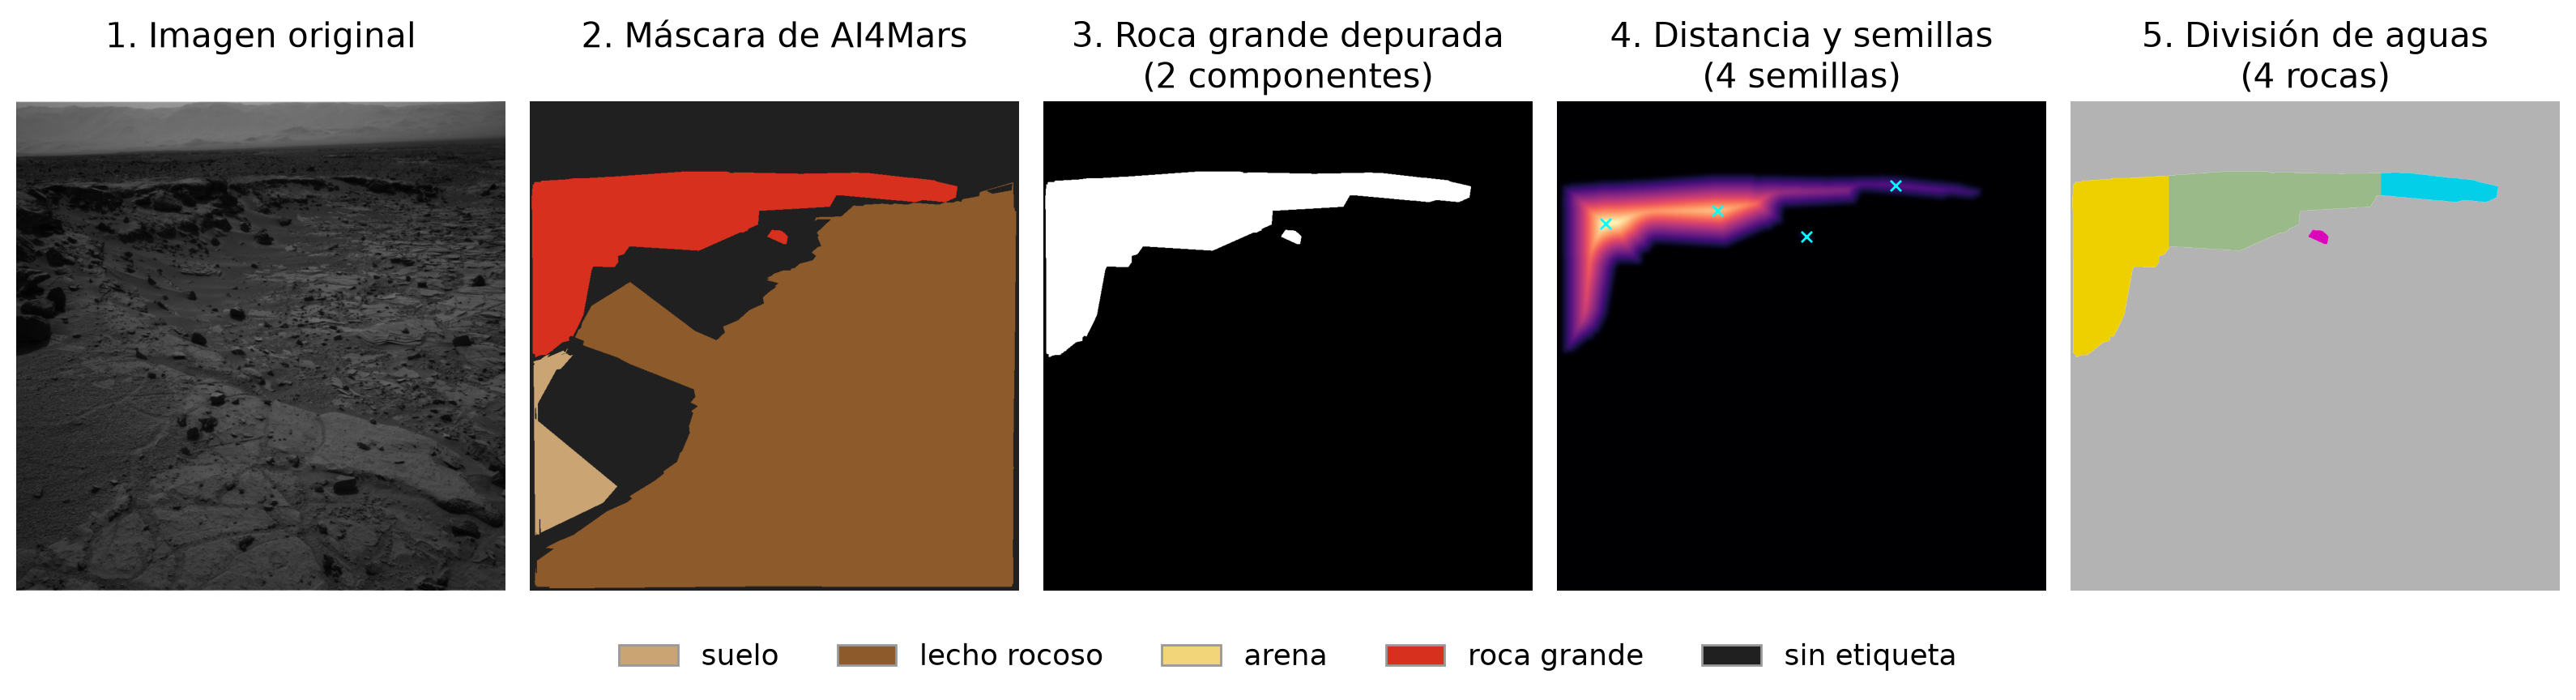
\includegraphics[width=\textwidth]{Figura_11_procedimiento_paso_a_paso.png}
  \caption[Procedimiento paso a paso]{Procedimiento paso a paso sobre una escena con
    varias rocas: imagen original, máscara de AI4Mars, binaria depurada, transformada de
    distancia con las semillas y resultado del conteo.}
  \label{fig:paso-a-paso}
\end{figure}

Cada imagen recibió una bandera de calidad que resume su aptitud para cada indicador
(Tabla~\ref{tab:banderas}, Figura~\ref{fig:banderas}).

\begin{table}[H]
  \centering
  \caption{Composición del conjunto según la bandera de calidad.}
  \label{tab:banderas}
  \begin{tabular}{llrr}
    \toprule
    \textbf{Bandera} & \textbf{Significado} & \textbf{Imágenes} & \textbf{\%} \\
    \midrule
    \texttt{ok}          & Contiene roca grande; apta para ambos indicadores & \cFlagOk     & \cFlagOkPct \\
    \texttt{no\_bigrock} & Contiene roca, pero sin roca grande que contar    & \cFlagNoBig  & \cFlagNoBigPct \\
    \texttt{no\_rock}    & Etiquetada, sin roca                             & \cFlagNoRock & \cFlagNoRockPct \\
    \texttt{mostly\_null}& Más del \SI{95}{\percent} sin etiqueta           & \cFlagNull   & \cFlagNullPct \\
    \texttt{empty}       & Sin ningún píxel etiquetado                      & \cFlagEmpty  & \cFlagEmptyPct \\
    \bottomrule
  \end{tabular}
\end{table}

\begin{figure}[H]
  \centering
  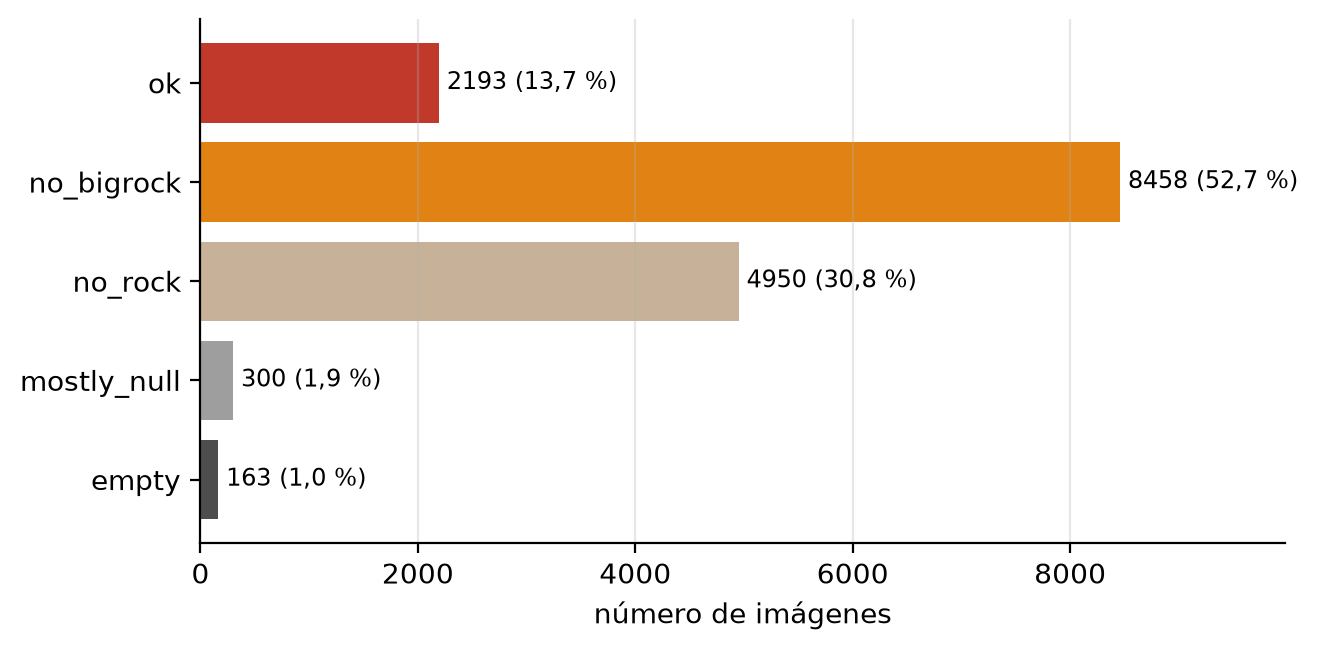
\includegraphics[width=0.82\textwidth]{Figura_12_banderas_calidad.png}
  \caption{Composición del conjunto analizado según la bandera de calidad.}
  \label{fig:banderas}
\end{figure}

Las banderas fijan las dos poblaciones de análisis, que se mantienen en todo el documento:

\begin{itemize}
  \item \textbf{Población de E1}: las \cNCobCalc{} escenas con al menos un píxel etiquetado,
    es decir, todas salvo las \cFlagEmpty{} de bandera \texttt{empty}.
  \item \textbf{Población de E2}: las \cFlagOk{} escenas de bandera \texttt{ok}. Quedan fuera
    las \cNNullBig{} escenas de bandera \texttt{mostly\_null} que contienen algún píxel de roca
    grande —y que aportarían \cRocasNullBig{} rocas—, porque cuando más del
    \SI{95}{\percent} de la escena carece de etiqueta la región de roca grande es un fragmento
    aislado cuya forma no puede interpretarse. La subsección~\ref{sec:diagnostico} muestra que
    los casos de anotación anómala identificados pertenecen precisamente a ese grupo.
\end{itemize}

La fracción de escena efectivamente etiquetada tiene una mediana de \cFracValidMed: algo más
de la mitad de cada imagen recibió etiqueta, y el resto corresponde al cuerpo del rover, al
cielo y a las distancias que el propio conjunto excluye por diseño.

\subsection{Cobertura de roca visible (E1)}

La cobertura pudo calcularse en \cNCobCalc{} de las \cNEscenas{} escenas (\cPctCobCalc);
\cNCobPos{} escenas (\cPctCobPos{} del total) presentaron cobertura de roca mayor que cero.
Entre estas últimas, la mediana de cobertura sobre píxeles etiquetados, según la
ecuación~\eqref{eq:cobertura}, fue del \cCobMedVal{} y la media del \cCobMediaVal; medida
sobre la imagen completa, la mediana es del \cCobMedTot{} y la media del \cCobMediaTot.

La distribución (Figura~\ref{fig:dist-cobertura}) es marcadamente \textbf{bimodal}: se
acumula en los extremos, con \cNCobCien{} escenas —el \cPctCobCien{} de las que contienen
roca— en las que la totalidad del área etiquetada es roca, y un segundo grupo de cobertura
nula. En total, \cNCobMitad{} escenas superan el \SI{50}{\percent} de cobertura.

\begin{figure}[H]
  \centering
  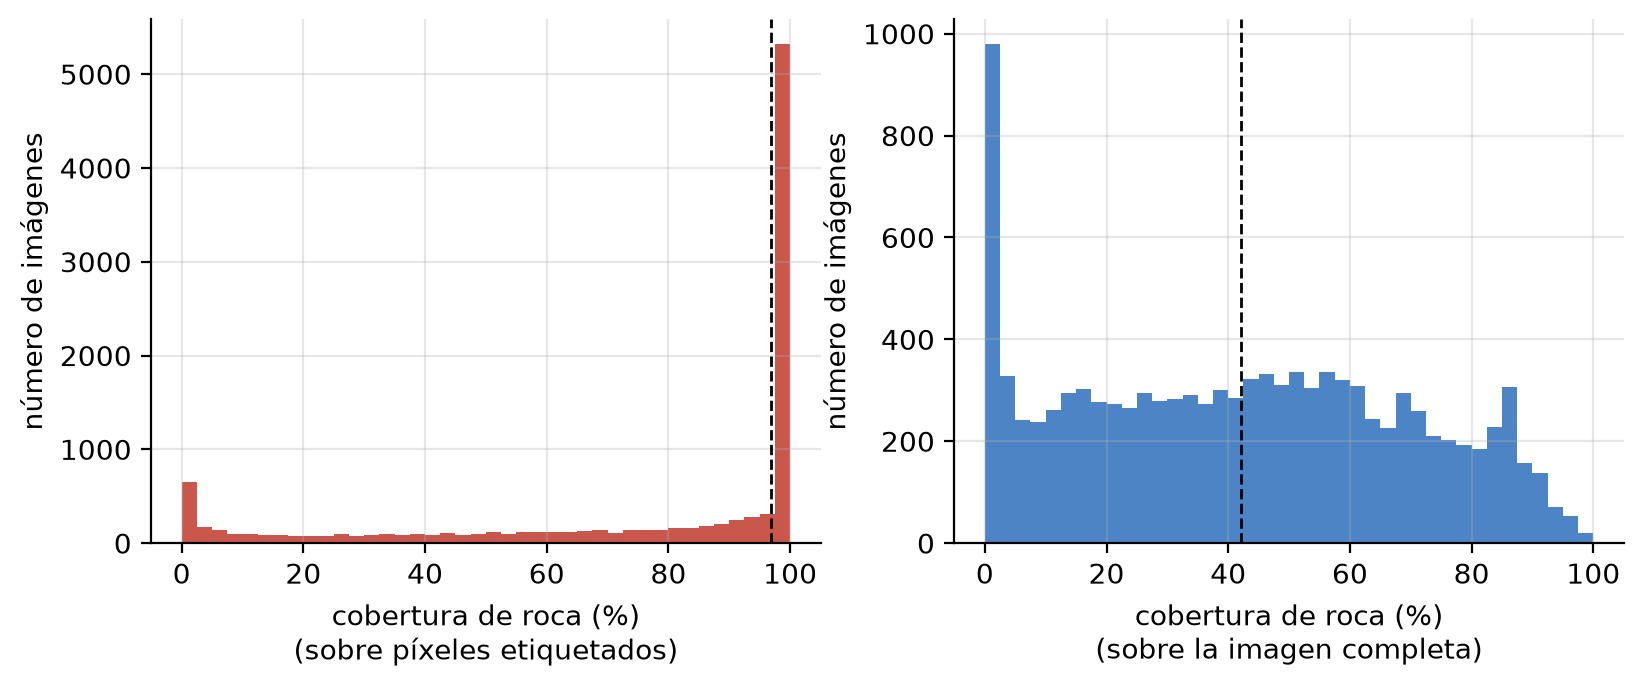
\includegraphics[width=\textwidth]{Figura_13_distribucion_cobertura.png}
  \caption[Distribución de la cobertura]{Distribución de la cobertura de roca visible en
    sus dos versiones: sobre píxeles etiquetados y sobre la imagen completa.}
  \label{fig:dist-cobertura}
\end{figure}

\subsubsection{Control del denominador}

La cobertura divide por los píxeles etiquetados. Si las escenas poco etiquetadas tendieran a
conservar sobre todo la roca, sus coberturas serían altas por construcción y no por el
terreno. Para examinarlo se relacionó la cobertura con la fracción de escena etiquetada
(Figura~\ref{fig:cob-vs-frac}) mediante las medidas de dependencia de la
Sección~\ref{sec:evaluacion}.

\begin{figure}[H]
  \centering
  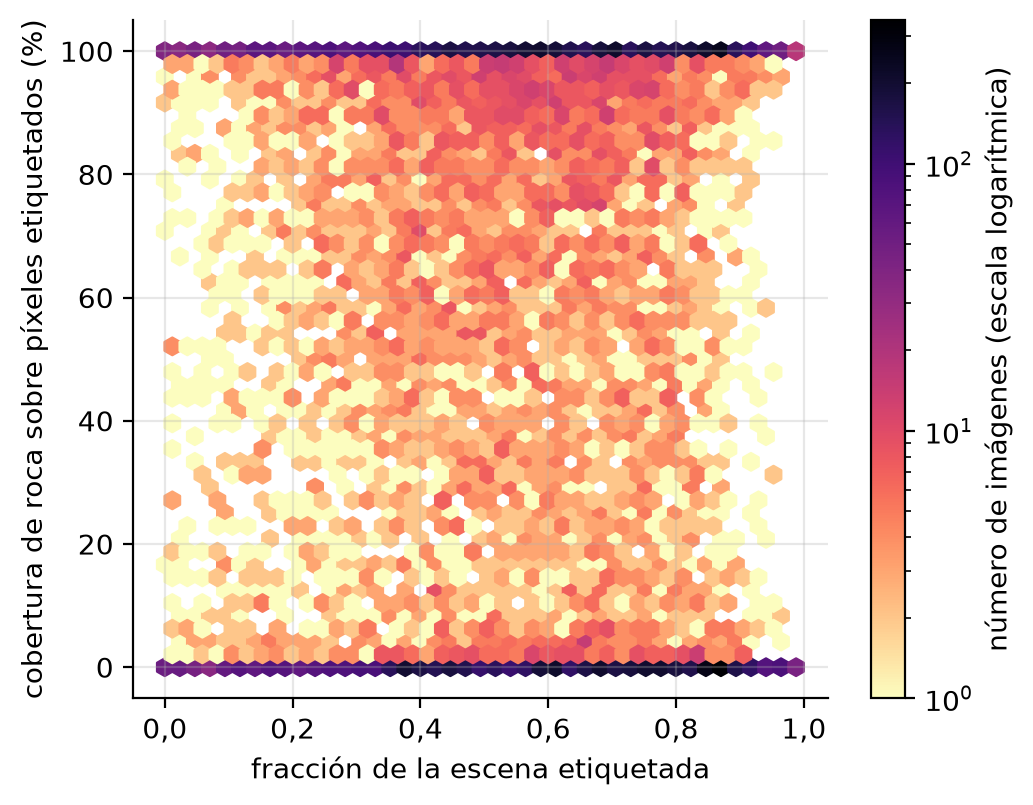
\includegraphics[width=0.85\textwidth]{Figura_14_cobertura_vs_fraccion_etiquetada.png}
  \caption{Cobertura frente a fracción de escena etiquetada.}
  \label{fig:cob-vs-frac}
\end{figure}

No se observó una asociación lineal global entre la cobertura y la fracción etiquetada
($r = \cDepFCPearson$, IC~95\,\% \cDepFCPearsonIC), por lo que no se encontró evidencia de
que las coberturas altas estén explicadas simplemente por una disminución lineal de la
fracción válida. Con \cDepFCN{} escenas, el intervalo excluye el cero: la asociación es
detectable, pero de una magnitud que explica menos de una milésima parte de la varianza. Las
medidas no lineales registran también una dependencia débil —correlación de distancia de
\cDepFCDcor, $p = \cDepFCDcorP$— que la Tabla~\ref{tab:dependencia} recoge junto al resto.
Este análisis no descarta otras formas de dependencia ni los sesgos propios del proceso de
anotación.

La descripción por tramos de fracción etiquetada (Tabla~\ref{tab:cob-por-frac}) aclara la
forma de esa dependencia. Si el artefacto del denominador operase, la cobertura mediana
debería ser máxima en las escenas menos etiquetadas y decrecer con la fracción. No ocurre:
crece hasta el tercer tramo y cae en el último, y las escenas con menos de un cuarto de
superficie etiquetada tienen una cobertura mediana inferior a la de los dos tramos
centrales.

\begin{table}[H]
  \centering
  \caption[Cobertura por tramos de fracción etiquetada]{Cobertura mediana por tramos de
    fracción de escena etiquetada, en sus dos versiones.}
  \label{tab:cob-por-frac}
  \begin{tabular}{lrcc}
    \toprule
     & & \multicolumn{2}{c}{\textbf{Cobertura mediana}} \\
    \cmidrule(lr){3-4}
    \textbf{Fracción etiquetada} & \textbf{Escenas} & \textbf{sobre lo etiquetado}
      & \textbf{sobre la imagen} \\
    \midrule
    hasta 0,25     & \cFTNA & \cFTMedA & \cFTMedTotA \\
    0,25 -- 0,50   & \cFTNB & \cFTMedB & \cFTMedTotB \\
    0,50 -- 0,75   & \cFTNC & \cFTMedC & \cFTMedTotC \\
    más de 0,75    & \cFTND & \cFTMedD & \cFTMedTotD \\
    \bottomrule
  \end{tabular}
\end{table}

\paragraph{Sensibilidad a la versión de la cobertura.} Se repitieron los análisis con la
cobertura sobre la imagen completa, cuyo denominador no depende de la anotación. Esa versión
sí depende fuertemente de la fracción etiquetada ($r = \cDepFTPearson$), como es inevitable:
una escena con poca superficie etiquetada no puede tener mucha roca etiquetada sobre el total.
Pese a ello, las conclusiones se mantienen. Las dos versiones ordenan las escenas de forma muy
parecida (correlación de rangos de \cSensRho); la diferencia entre máscaras colaborativas y de
experto persiste, con medianas del \cSensTotColab{} y del \cSensTotExp{} en las escenas con
roca ($p \cSensTotP$ en la prueba de Mann-Whitney); y la ausencia de asociación con el conteo
se reproduce ($r = \cSensConteoPearson$, $p = \cSensConteoPearsonP$; $\rho =
\cSensConteoSpearman$, $p = \cSensConteoSpearmanP$).

\subsection{Conteo aproximado de rocas individuales (E2)}

El conteo se aplicó a las \cFlagOk{} escenas de la población de E2 y arrojó un total de
\cNRocas{} rocas, con una mediana de una roca por imagen y un máximo de \cRocasMax. La
Tabla~\ref{tab:bandas-conteo} y la Figura~\ref{fig:bandas-conteo} recogen la distribución.

\begin{table}[H]
  \centering
  \caption[Distribución del conteo de rocas]{Distribución del conteo de rocas sobre las
    \cFlagOk{} escenas de la población de E2.}
  \label{tab:bandas-conteo}
  \begin{tabular}{lrr}
    \toprule
    \textbf{Rocas por imagen} & \textbf{Imágenes} & \textbf{\%} \\
    \midrule
    0 (descartadas por los filtros) & \cBandaCero        & \cBandaCeroPct \\
    1                               & \cBandaUna         & \cBandaUnaPct \\
    2--3                            & \cBandaDosTres     & \cBandaDosTresPct \\
    4--9                            & \cBandaCuatroNueve & \cBandaCuatroNuevePct \\
    10 o más                        & \cBandaDiez        & \cBandaDiezPct \\
    \midrule
    Total de rocas                  & \multicolumn{2}{r}{\cNRocas} \\
    \bottomrule
  \end{tabular}
\end{table}

\begin{figure}[H]
  \centering
  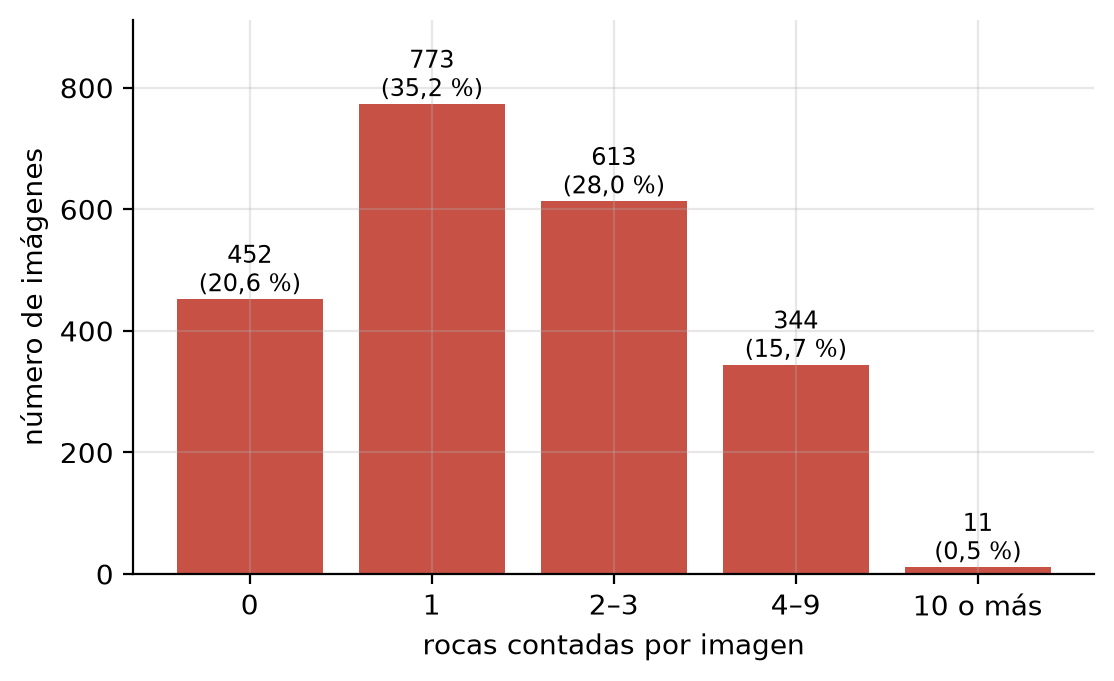
\includegraphics[width=0.82\textwidth]{Figura_15_conteo_por_bandas.png}
  \caption{Distribución del conteo de rocas por imagen.}
  \label{fig:bandas-conteo}
\end{figure}

En \cBandaCero{} escenas —el \cBandaCeroPct\,\% de la población— existen píxeles de roca
grande pero ninguna región supera los filtros de área mínima y forma. La
subsección~\ref{sec:diagnostico} examina esas escenas; el dato se reporta explícitamente
porque delimita el alcance real del indicador.

En promedio, cada escena contiene \cRawMedio{} componentes conectadas antes de la división de
aguas y \cRocasMedio{} rocas después. El paso de división de aguas \textbf{no aumenta} el
conteo promedio, porque el aumento que produce al separar regiones unidas queda compensado por
las componentes que los filtros descartan. Es coherente con que el criterio de prominencia
evitara la fragmentación masiva que producía la detección de máximos por separación mínima
(Sección~\ref{sec:calibracion}), aunque, como se verá, no la eliminó por completo.

\subsubsection{Distribución tamaño--frecuencia}

Clasificando las \cNRocas{} rocas según su tamaño relativo al área de la imagen
(Tabla~\ref{tab:tamanos}, Figura~\ref{fig:tamano-frecuencia}) se obtiene una
\textbf{distribución decreciente}: predominan las rocas pequeñas y la frecuencia disminuye
al aumentar el tamaño.

\begin{table}[H]
  \centering
  \caption{Distribución tamaño--frecuencia de las rocas contadas.}
  \label{tab:tamanos}
  \begin{tabular}{lrr}
    \toprule
    \textbf{Clase de tamaño} & \textbf{Rocas} & \textbf{\%} \\
    \midrule
    Pequeña (\textless\ \SI{0.5}{\percent} del área) & \cTamPeq & \cTamPeqPct \\
    Mediana (\SI{0.5}{\percent} -- \SI{2}{\percent})  & \cTamMed & \cTamMedPct \\
    Grande ($\geq$ \SI{2}{\percent})                  & \cTamGra & \cTamGraPct \\
    \bottomrule
  \end{tabular}
\end{table}

\begin{figure}[H]
  \centering
  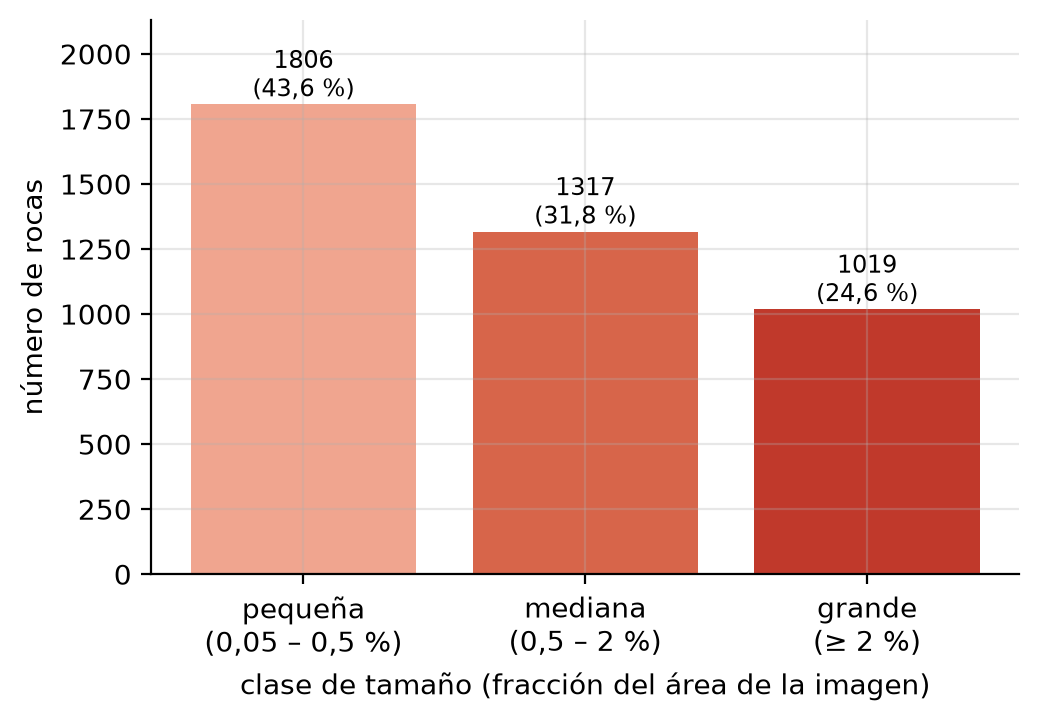
\includegraphics[width=0.82\textwidth]{Figura_16_tamano_frecuencia.png}
  \caption{Distribución tamaño--frecuencia de las rocas contadas.}
  \label{fig:tamano-frecuencia}
\end{figure}

Esta forma coincide cualitativamente con las distribuciones tamaño--frecuencia descritas en
los estudios de abundancia de rocas en sitios de aterrizaje
\citep{golombek2003mer, lorenz2023analytic}. La coincidencia debe leerse con cautela: aquí los
tamaños son \textbf{relativos al campo de visión} y no métricos, porque el procedimiento no
dispone de la escala de la escena. La comparación es de forma, no de magnitud.

La solidez media de las regiones aceptadas es de \cSolidezMedia, es decir, formas compactas;
de las \cNConRocas{} escenas con al menos una roca, solo \cNSolidezBaja{} presentan solidez
media inferior a $0{,}7$, señal de contornos cóncavos o de regiones posiblemente subdivididas
en exceso.

\subsection{Relación entre cobertura y conteo (H4)}
\label{sec:dependencia}

La hipótesis H4 sostiene que los dos indicadores aportan información distinta. Un coeficiente
de Pearson próximo a cero no basta para afirmarlo, porque solo excluye la asociación lineal.
La Tabla~\ref{tab:dependencia} reúne las medidas de dependencia descritas en la
Sección~\ref{sec:evaluacion} para este par y para el control del denominador.

\begin{table}[H]
  \centering
  \small
  \caption[Medidas de dependencia]{Medidas de dependencia entre cobertura y conteo, y entre
    fracción etiquetada y cobertura. Intervalos por \textit{bootstrap} y valores $p$ por
    permutación; la información mutua se compara con el percentil 95 de su distribución
    bajo independencia.}
  \label{tab:dependencia}
  \begin{tabular}{llcc}
    \toprule
    \textbf{Medida} & \textbf{Qué detecta} & \textbf{Cobertura--conteo} & \textbf{Fracción--cobertura} \\
     & & ($n = \cDepCCN$) & ($n = \cDepFCN$) \\
    \midrule
    Pearson $r$       & lineal    & \cDepCCPearson{} \cDepCCPearsonIC & \cDepFCPearson{} \cDepFCPearsonIC \\
                      &           & $p = \cDepCCPearsonP$ & $p = \cDepFCPearsonP$ \\
    Spearman $\rho$   & monótona  & \cDepCCSpearman{} \cDepCCSpearmanIC & \cDepFCSpearman{} \cDepFCSpearmanIC \\
                      &           & $p = \cDepCCSpearmanP$ & $p = \cDepFCSpearmanP$ \\
    Kendall $\tau$    & monótona  & \cDepCCKendall{} ($p = \cDepCCKendallP$) & \cDepFCKendall{} ($p = \cDepFCKendallP$) \\
    Correlación de distancia & cualquiera & \cDepCCDcor{} ($p = \cDepCCDcorP$) & \cDepFCDcor{} ($p = \cDepFCDcorP$)$^{a}$ \\
    Información mutua (bits) & cualquiera & \cDepCCIM{} (nula \cDepCCIMNula) & \cDepFCIM{} (nula \cDepFCIMNula) \\
                      &           & $p = \cDepCCIMP$ & $p = \cDepFCIMP$ \\
    \bottomrule
    \multicolumn{4}{l}{\footnotesize $^{a}$ Sobre una submuestra aleatoria de \cDepDcorSub{}
      escenas, por coste de cómputo.}
  \end{tabular}
\end{table}

Los indicadores presentan una \textbf{asociación lineal prácticamente nula} en las escenas
analizadas ($r = \cDepCCPearson$), y tampoco muestran asociación monótona ($\rho =
\cDepCCSpearman$, $p = \cDepCCSpearmanP$). Sin embargo, \textbf{no son estadísticamente
independientes}: la correlación de distancia ($\cDepCCDcor$, $p = \cDepCCDcorP$) y la
información mutua ($p = \cDepCCIMP$) detectan una dependencia débil que los coeficientes de
correlación no capturan. La prueba chi-cuadrado sobre la tabla de contingencia por tramos, más
gruesa, queda en el límite ($\chi^2 = \cChiDos$ con \cChiGl{} grados de libertad,
$p = \cChiP$; V de Cramér \cCramer).

La Tabla~\ref{tab:conteo-por-cobertura} muestra la forma de esa dependencia: una \textbf{U
invertida}. El conteo medio es bajo en las escenas de cobertura muy baja, alcanza su máximo
entre el \SI{10}{\percent} y el \SI{50}{\percent} de cobertura y vuelve a bajar en las escenas
de cobertura total. Los dos extremos tienen explicaciones distintas. En el inferior la relación
es en parte de construcción: los píxeles de roca grande forman parte del numerador de la
cobertura, de modo que una cobertura muy baja implica una región de roca grande pequeña, que
los filtros de área descartan con frecuencia. En el superior, una escena enteramente cubierta
de roca suele ser un afloramiento continuo, que el anotador marca como lecho rocoso y no como
bloques discretos.

\begin{table}[H]
  \centering
  \caption[Conteo según el tramo de cobertura]{Conteo de rocas según el tramo de cobertura,
    sobre la población de E2.}
  \label{tab:conteo-por-cobertura}
  \begin{tabular}{lrccc}
    \toprule
    \textbf{Cobertura} & \textbf{Escenas} & \textbf{Conteo medio} & \textbf{Sin rocas (\%)}
      & \textbf{Cuatro o más (\%)} \\
    \midrule
    hasta \SI{10}{\percent}              & \cUNA & \cUMediaA & \cUCeroA & \cUCuatroA \\
    \SI{10}{\percent} -- \SI{50}{\percent} & \cUNB & \cUMediaB & \cUCeroB & \cUCuatroB \\
    \SI{50}{\percent} -- \SI{80}{\percent} & \cUNC & \cUMediaC & \cUCeroC & \cUCuatroC \\
    \SI{80}{\percent} -- \SI{99.99}{\percent} & \cUND & \cUMediaD & \cUCeroD & \cUCuatroD \\
    \SI{100}{\percent}                   & \cUNE & \cUMediaE & \cUCeroE & \cUCuatroE \\
    \bottomrule
  \end{tabular}
\end{table}

La magnitud de la dependencia se mide con la razón de correlación. Los deciles de cobertura
explican el \cEtaConteo{} de la varianza del conteo, frente a un \cEtaConteoNula{} esperable
por azar ($p = \cEtaConteoP$ por permutación); las bandas de conteo explican el \cEtaCob{} de
la varianza de la cobertura, valor que no se distingue del azar ($p = \cEtaCobP$). Conocer uno
de los indicadores informa, por tanto, muy poco sobre el otro: ninguno es función del otro y
los dos describen aspectos distintos del terreno, cuánta roca hay y cuántos bloques discretos
la componen. Pero la relación existe, no es lineal, y en parte procede de cómo se definen.

\subsection{Composición del terreno y tipología de escenas (E3)}

Además de los dos indicadores previstos, cada imagen se caracterizó por la proporción de
cada clase sobre sus píxeles etiquetados. La composición media es de \cCompBed{} de lecho
rocoso, \cCompSoil{} de suelo, \cCompSand{} de arena y \cCompBig{} de roca grande. La clase
dominante es el lecho rocoso en \cDomBed{} imágenes, el suelo en \cDomSoil, la arena en
\cDomSand{} y la roca grande en apenas \cDomBig.

A partir de esa composición se definió la tipología de la Tabla~\ref{tab:tipologia}, que la
Figura~\ref{fig:tipologia} representa.

\begin{table}[H]
  \centering
  \caption{Tipología de escenas según la composición del terreno.}
  \label{tab:tipologia}
  \begin{tabular}{llrr}
    \toprule
    \textbf{Tipo} & \textbf{Criterio} & \textbf{Imágenes} & \textbf{\%} \\
    \midrule
    Rocoso  & roca $\geq$ \SI{66}{\percent}   & \cTipoRocoso  & \cTipoRocosoPct \\
    Suelo   & suelo $\geq$ \SI{50}{\percent}  & \cTipoSuelo   & \cTipoSueloPct \\
    Arenoso & arena $\geq$ \SI{50}{\percent}  & \cTipoArenoso & \cTipoArenosoPct \\
    Mixto   & ninguna clase predomina         & \cTipoMixto   & \cTipoMixtoPct \\
    Sin etiqueta & sin píxeles clasificados    & \cTipoSinEtiq & \cTipoSinEtiqPct \\
    \bottomrule
  \end{tabular}
\end{table}

\begin{figure}[H]
  \centering
  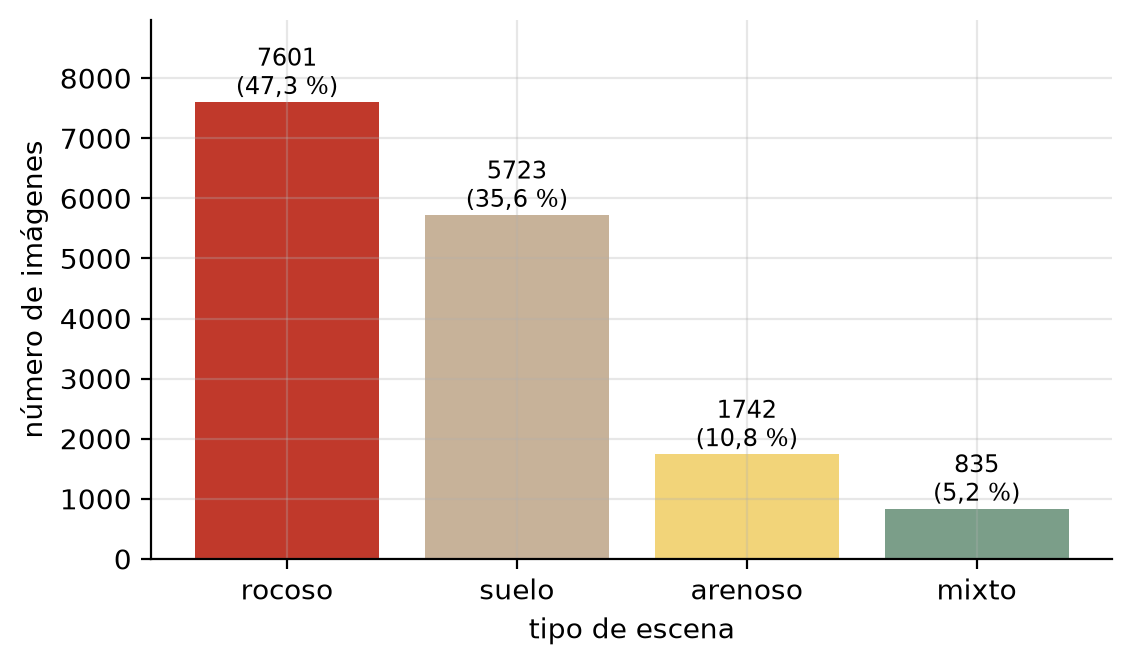
\includegraphics[width=0.82\textwidth]{Figura_17_tipologia_escenas.png}
  \caption{Tipología de escenas según la composición del terreno.}
  \label{fig:tipologia}
\end{figure}

\subsection{Variación a lo largo de la secuencia de adquisición (E3)}

El orden temporal se obtiene del \textbf{reloj de nave}, el contador de a bordo que el
identificador de cada imagen incluye tras el prefijo de cámara y que se registra en la columna
\texttt{sclk} del conjunto de resultados. Ordenando las imágenes por ese contador y
agrupándolas en tramos de igual número de imágenes, se observa (Figura~\ref{fig:secuencia})
una \textbf{alternancia clara entre segmentos de la secuencia francamente rocosos y segmentos
de suelo o arena}, con concentraciones puntuales de roca grande que alcanzan hasta el
\SI{40}{\percent} de las imágenes de un segmento.

\begin{figure}[H]
  \centering
  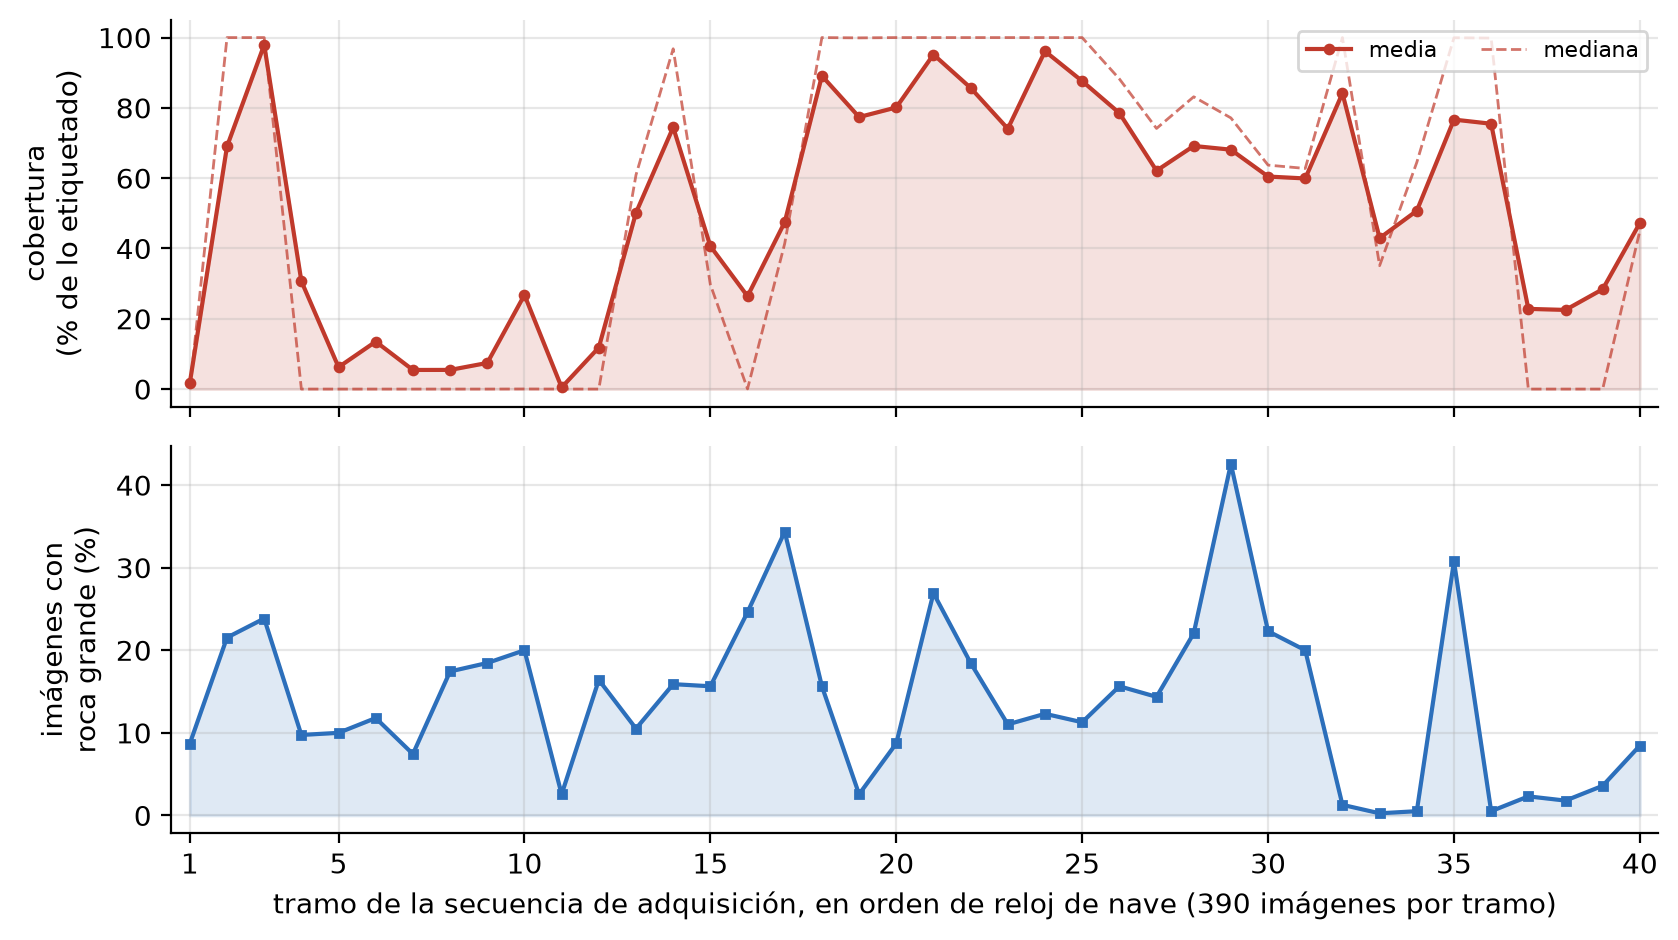
\includegraphics[width=\textwidth]{Figura_18_variacion_secuencia.png}
  \caption[Variación a lo largo de la secuencia de adquisición]{Cobertura y presencia de roca
    grande a lo largo de la secuencia de adquisición, en segmentos de igual número de
    imágenes ordenados por el reloj de nave.}
  \label{fig:secuencia}
\end{figure}

Esta lectura debe interpretarse como una \textbf{ordenación relativa en el tiempo} y no como
una variación espacial. El orden cronológico de las imágenes no equivale a distancia recorrida:
el rover puede tomar muchas imágenes desde una misma ubicación, con orientaciones distintas, y
el conjunto no incluye la posición desde la que se adquirió cada una. Por ello el análisis no
permite afirmar en qué lugares del trayecto se concentra la roca, solo en qué momentos de la
secuencia de adquisición.

Cabe señalar que el subconjunto es casi enteramente de la cámara izquierda del par estéreo
—\cNOjoIzq{} imágenes frente a \cNOjoDer{} de la derecha—, por lo que no fue posible la
comparación entre ojos que E3 contemplaba.

\subsection{Extensión aplicada: reglas heurísticas de priorización}
\label{sec:extension}

Como extensión aplicada, y fuera del núcleo de la pregunta de investigación, los indicadores se
tradujeron en seis reglas heurísticas de priorización con umbrales explícitos, y se construyó
una aplicación de escritorio para consultar el conjunto de resultados. Aplicadas al conjunto,
las reglas sitúan \cPrioAlta{} escenas en prioridad alta, \cPrioMedia{} en media y
\cPrioBaja{} en baja; las \cPrioSin{} restantes no activan ninguna regla de prioridad.

Estas reglas \textbf{no constituyen una evaluación de riesgo para la navegación} ni están
calibradas para ella. Sin escala métrica no puede inferirse la altura de un bloque, la
transitabilidad, el daño potencial a las ruedas ni la probabilidad de atrapamiento a partir de
porcentajes de píxeles, y no existe para este subconjunto un registro de incidentes contra el
que validarlas. Su función es ordenar escenas para revisión con un criterio visible y
ajustable. El Anexo~\ref{app:extension} documenta las reglas, su distribución y la aplicación.

\section{Evaluación y validación}

\subsection{Contraste con las máscaras de experto (H3)}
\label{sec:experto}

El conjunto incluye \cNGold{} máscaras etiquetadas por especialistas con acuerdo del
\SI{100}{\percent}, sobre imágenes que \textbf{no} forman parte del conjunto de entrenamiento.
Se ejecutó sobre ellas el mismo procedimiento, sin modificar ningún parámetro
(Tabla~\ref{tab:validacion}, Figura~\ref{fig:validacion}).

\begin{table}[H]
  \centering
  \caption[Indicadores según la fuente de etiqueta]{Indicadores según la fuente de etiqueta.
    Las dos columnas corresponden a imágenes distintas.}
  \label{tab:validacion}
  \begin{tabular}{lcc}
    \toprule
    \textbf{Indicador} & \textbf{Colaborativas} & \textbf{Experto} \\
     & ($n = \cNEscenas$) & ($n = \cNGold$) \\
    \midrule
    Cobertura mediana (escenas con roca)          & \cCobMedVal     & \cGoldCobMedPos \\
    Escenas con cobertura del \SI{100}{\percent}  & \cColabPctCien  & \cGoldPctCien \\
    Lecho rocoso (media sobre lo etiquetado)      & \cColabBed      & \cGoldBed \\
    Suelo y arena (media sobre lo etiquetado)     & \cColabSueloArena & \cGoldSueloArena \\
    Escenas con roca grande                       & \cPctBigAny     & \cGoldUnoBig \\
    Fracción etiquetada (mediana)                 & \cFracValidMed  & \cFracValidGold \\
    \bottomrule
  \end{tabular}
\end{table}

\begin{figure}[H]
  \centering
  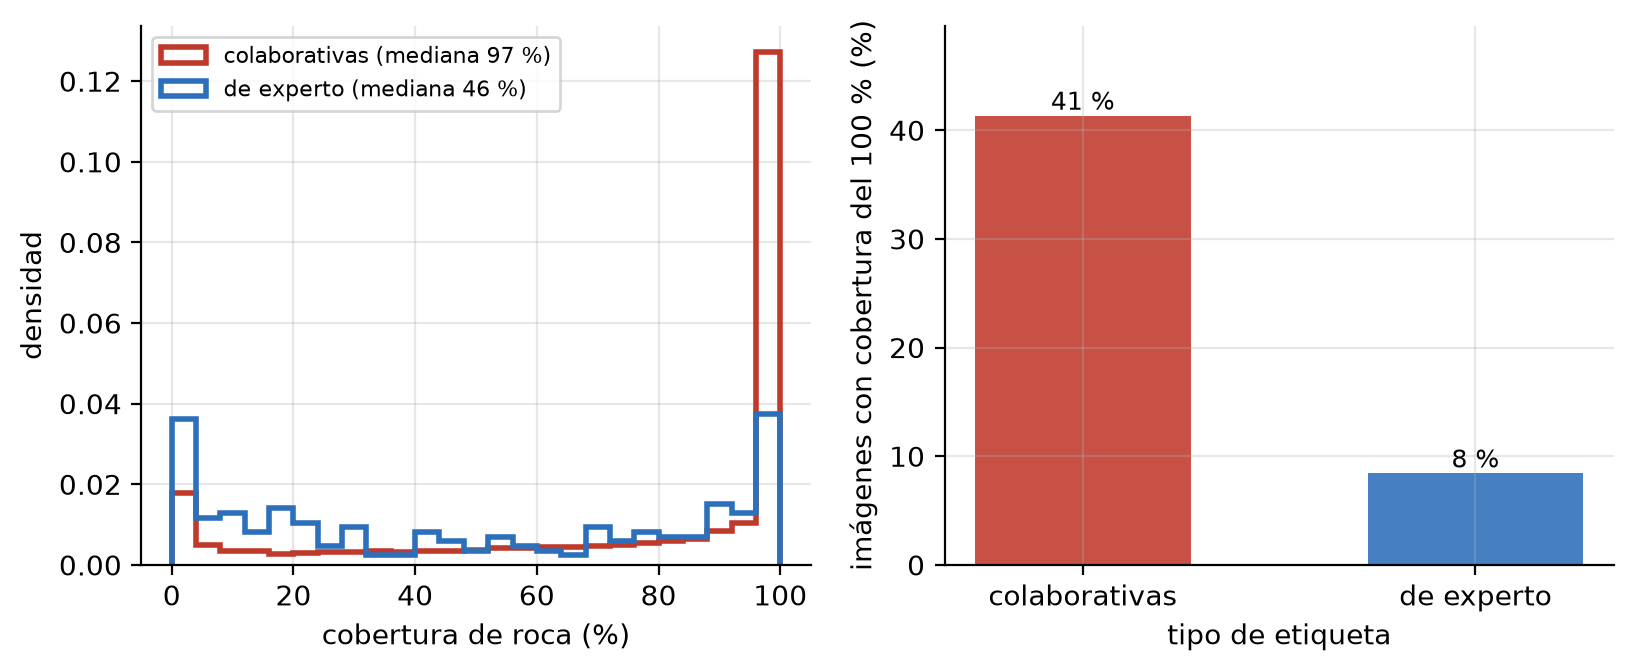
\includegraphics[width=0.85\textwidth]{Figura_19_validacion_experto.png}
  \caption[Cobertura según la fuente de etiqueta]{Cobertura según la fuente de etiqueta, en
    las escenas con roca. Las dos distribuciones proceden de muestras de imágenes distintas.}
  \label{fig:validacion}
\end{figure}

\paragraph{Resultado.} Las dos fuentes de anotación presentan distribuciones muy diferentes de
cobertura y de clases. La diferencia de medianas en las escenas con roca es de
\cFuenteDifMed{} puntos porcentuales (IC~95\,\% \cFuenteDifIC; $p \cFuenteMWp$ en la prueba de
Mann-Whitney). En cambio, la fracción etiquetada es prácticamente igual en ambas fuentes
(\cFracValidMed{} frente a \cFracValidGold, $p = \cFracValidP$).

Esta comparación no permite, por sí sola, atribuir la diferencia a la anotación. Las máscaras de
experto cubren \textbf{otras imágenes}, para las que AI4Mars no distribuye máscara
colaborativa, de modo que no es posible comparar las dos fuentes sobre las mismas escenas. Una
diferencia de cobertura puede deberse a que cada grupo anote de forma distinta o a que las dos
muestras contengan terreno distinto.

\paragraph{Instrumento común.} Para separar ambos efectos se aplicó el segmentador entrenado,
que es una función fija de la imagen, a la región anotable de \cFANColab{} escenas
colaborativas no vistas en su entrenamiento y de las \cFANExp{} de experto, según el diseño de
la Sección~\ref{sec:evaluacion}. La Tabla~\ref{tab:instrumento} y la
Figura~\ref{fig:instrumento} presentan el resultado.

\begin{table}[H]
  \centering
  \caption[Descomposición de la diferencia entre fuentes]{Cobertura según la etiqueta y según
    el instrumento común, en las dos muestras de imágenes, y descomposición de la diferencia
    de medias. Intervalos por \textit{bootstrap}.}
  \label{tab:instrumento}
  \small
  \begin{tabular}{lcc}
    \toprule
     & \textbf{Muestra colaborativa} & \textbf{Muestra de experto} \\
     & ($n = \cFANColab$) & ($n = \cFANExp$) \\
    \midrule
    Cobertura según la etiqueta, media (mediana)        & \cFAEtiqMediaColab{} (\cFAEtiqMedColab) & \cFAEtiqMediaExp{} (\cFAEtiqMedExp) \\
    Cobertura según el instrumento, media (mediana)     & \cFARegMediaColab{} (\cFARegMedColab)   & \cFARegMediaExp{} (\cFARegMedExp) \\
    Etiqueta menos instrumento, media                   & \cResColab{} p.p. & \cResExp{} p.p. \\
    \midrule
    \multicolumn{3}{l}{\textit{Descomposición de la diferencia de medias entre muestras}} \\
    Diferencia total según la etiqueta  & \multicolumn{2}{c}{\cDescTotal{} p.p.} \\
    Atribuible a las imágenes           & \multicolumn{2}{c}{\cDescImg{} p.p. \cDescImgIC{} (\cDescImgPct)} \\
    Atribuible a la anotación           & \multicolumn{2}{c}{\cDescAnot{} p.p. \cDescAnotIC{} (\cDescAnotPct)} \\
    \bottomrule
  \end{tabular}
\end{table}

\begin{figure}[H]
  \centering
  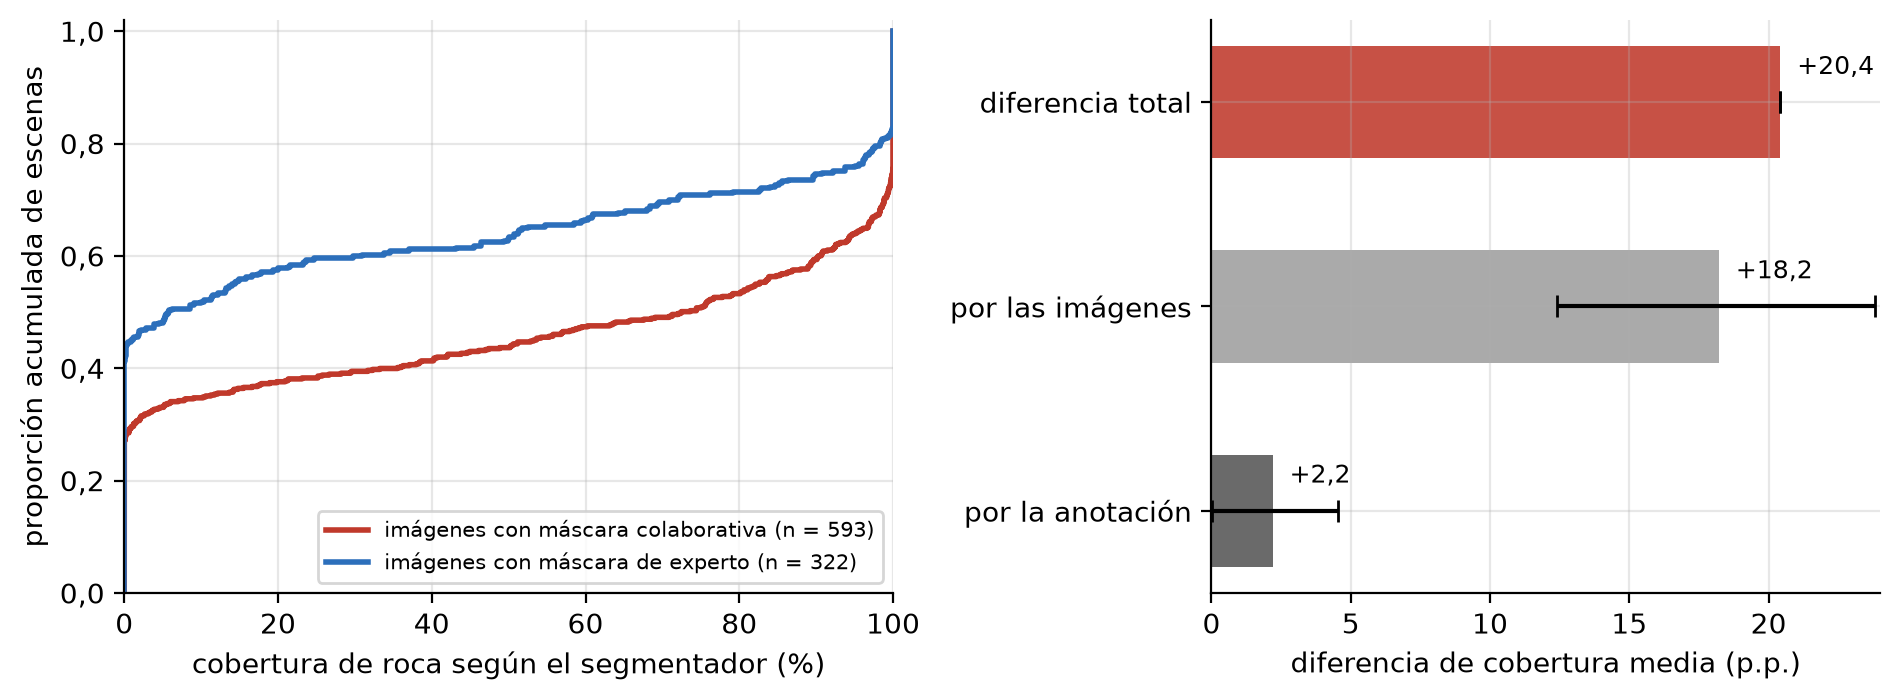
\includegraphics[width=\textwidth]{Figura_30_instrumento_comun.png}
  \caption[Instrumento común sobre las dos muestras]{Izquierda: distribución acumulada de la
    cobertura que el segmentador asigna a la región anotable de cada escena, sin intervención
    de ninguna etiqueta. Derecha: descomposición de la diferencia de cobertura media entre las
    dos muestras, con intervalos del \SI{95}{\percent}.}
  \label{fig:instrumento}
\end{figure}

El instrumento común reproduce la mayor parte de la diferencia sin pasar por ninguna anotación.
Medidas por el mismo segmentador, las imágenes de la muestra de experto tienen una cobertura
mediana del \cFARegMedExp{} frente al \cFARegMedColab{} de la muestra colaborativa: \textbf{el
conjunto de máscaras de experto está compuesto por escenas mucho menos rocosas}. De la
diferencia total de medias, \cDescImg{} puntos —el \cDescImgPct— se asocian con la composición
de las muestras de imágenes y \cDescAnot{} puntos —el \cDescAnotPct— con la fuente de las
etiquetas. Esta segunda componente es pequeña y su intervalo apenas excluye el cero. Ambas
anotaciones asignan algo menos de roca que el instrumento, la colaborativa \cResColab{} puntos y
la de experto \cResExp: la diferencia entre ambos residuos es la componente de anotación.

\paragraph{Sensibilidad.} La conclusión no depende de la muestra ni del instrumento concretos.
Tomando la muestra colaborativa solo de los bloques temporales de prueba ($n = \cFPNColab$), a más
de un sol de cualquier imagen de entrenamiento, la componente de imágenes es el \cFPDescImgPct{}
y la de anotación \cFPDescAnot{} puntos \cFPDescAnotIC. Con el segmentador de una versión
anterior, entrenado con un reparto al azar por imagen, la descomposición atribuía a las imágenes
el \cFVDescImgPct{} y a la anotación \cFVDescAnot{} puntos \cFVDescAnotIC. En todos los casos la
mayor parte de la diferencia procede de las imágenes y la componente de anotación es pequeña y
positiva; su magnitud exacta, entre dos y cuatro puntos, depende del instrumento.

Las imágenes de experto no proceden de un periodo distinto de la misión: la mediana de la
distancia, en reloj de nave, a la imagen de entrenamiento más próxima es de \cFugaExpSoles{}
soles. La diferencia de composición refleja, por tanto, cómo se seleccionaron las escenas del
conjunto de prueba, algo que la documentación del conjunto no especifica y este trabajo no
puede determinar.

La descomposición tiene un supuesto que conviene explicitar: que el instrumento responde igual
a las dos muestras. Como el segmentador se entrenó con etiquetas colaborativas, puede haber
heredado parte del criterio de esa anotación; si así fuera, aplicado a las imágenes de experto
tendería a asignarles más roca de la que el experto marca, y la componente atribuida a la
anotación quedaría subestimada. Es lo que se observa: frente al experto, el modelo sobreestima
la cobertura en \cBAExpMedia{} puntos de media (Sección~\ref{sec:modelo-experto}). La cifra de
\cDescAnot{} puntos debe leerse, por tanto, como una estimación aproximada y probablemente
conservadora.

\paragraph{Interpretación.} Dado que el mismo cálculo se aplicó a ambas fuentes, la diferencia
observada no puede atribuirse a la implementación de la fórmula; según el instrumento común, se
asocia principalmente con la composición de las muestras de imágenes y, en menor medida, con la
fuente de las etiquetas. La componente de anotación es compatible con la hipótesis de un
\textbf{sesgo de saliencia} en la anotación colaborativa —que las regiones visualmente
prominentes, como la roca, reciban una anotación más consistente o completa—, pero el diseño
del estudio no permite identificar causalmente ese mecanismo: no se midieron la atención, la
fatiga ni el tiempo de anotación. Un mecanismo alternativo que se había planteado, que la
anotación colaborativa dejara sin etiquetar más suelo y arena y eso redujera el denominador,
\textbf{no encuentra apoyo}: la fracción etiquetada es igual en las dos fuentes.

\subsection{Validación con conteo humano (H2)}
\label{sec:validacion-manual}

La metodología comprometía un contraste entre el conteo automático y un conteo manual, con el
diseño descrito en la Sección~\ref{sec:evaluacion}. Se realizó en dos rondas: una piloto de
\num{24} escenas y una definitiva de \cVN{} escenas, que es la que se reporta. Los parámetros
estaban congelados antes de la primera respuesta y ninguna escena de calibración forma parte de
la muestra definitiva (Sección~\ref{sec:calibracion}). La validación la realizó un único
observador, de modo que lo que sigue es \textbf{una evaluación exploratoria} y no una medición
de exactitud.

\paragraph{Correcciones derivadas de la ronda piloto.} La ronda piloto empleaba cuatro bandas,
la última abierta en «diez o más». Ese diseño resultó defectuoso: un procedimiento que contara
ochenta rocas donde el observador distinguía una decena puntuaba como acierto exacto, de modo
que la escala \textbf{favorecía sistemáticamente a los métodos que sobreestiman}. La ronda
definitiva subdivide esa banda. Corrige además otros tres defectos: excluye las escenas cuya
región anotada no alcanza los \num{2000} píxeles —en la ronda piloto siete de veinticuatro eran
imperceptibles—, sustituye el relleno opaco por un tinte tenue que no oculta la textura, y
estratifica la muestra por área de la región en lugar de por la banda del propio
procedimiento.

\subsubsection{Resultado}

Sobre las \cVN{} escenas, el acuerdo exacto de banda es del \cVAcuerdo, con coeficiente kappa
de Cohen de \cVKappa{} (IC~95\,\% \cVKappaIC) y kappa ponderado de \cVKappaPond{} (IC~95\,\%
\cVKappaPondIC). Ambos corresponden a un acuerdo \textbf{escaso} en la escala de
\citet{landis1977}. El acuerdo aparente es engañoso: \cVCoincUnaTres{} de las \cVCoinc{}
coincidencias se concentran en una sola celda, la de una a tres rocas.

El desacuerdo es \textbf{marcadamente asimétrico}. El procedimiento sitúa la escena en una
banda inferior a la del observador en \cVAbajo{} casos y superior en solo \cVArriba{}
($p \cVSignoP$ en la prueba de signos). La Figura~\ref{fig:validacion-manual} muestra la
matriz de acuerdo.

\begin{figure}[H]
  \centering
  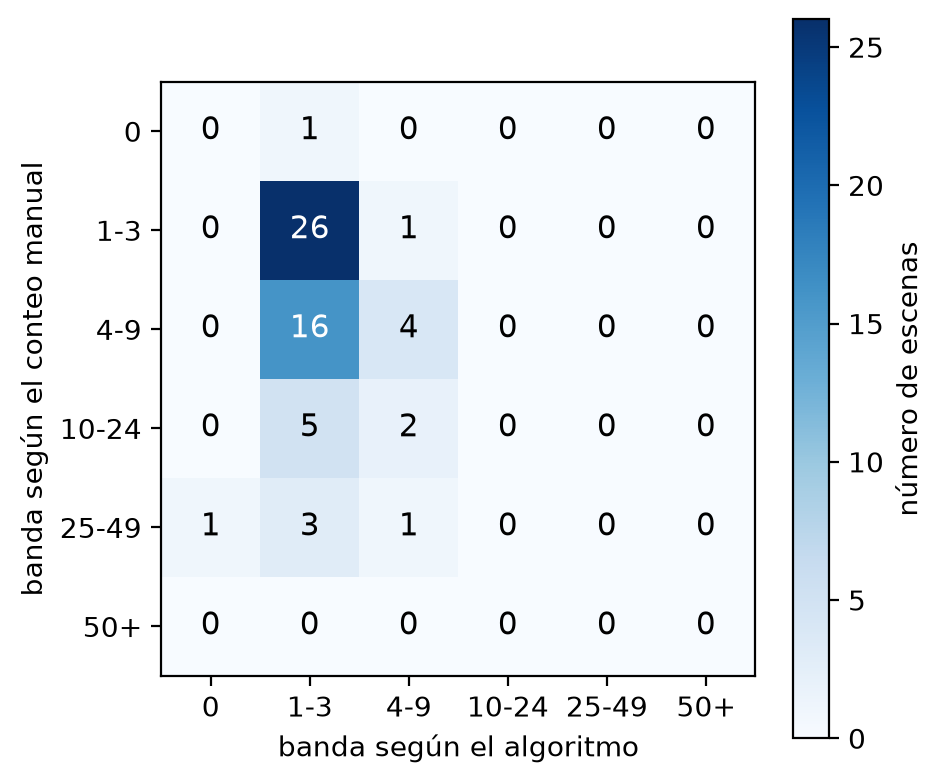
\includegraphics[width=0.78\textwidth]{Figura_26_validacion_manual_v2.png}
  \caption[Acuerdo entre el conteo manual y el automático]{Matriz de acuerdo entre el
    conteo manual por bandas y el automático, sobre \cVN{} escenas. Las tres columnas de
    la derecha están vacías: con los parámetros fijados, el procedimiento no produce ningún
    conteo superior a nueve.}
  \label{fig:validacion-manual}
\end{figure}

El rasgo más visible de esa matriz son las \textbf{tres columnas vacías}. En ninguna de las
\cVN{} escenas el procedimiento devuelve más de \cVMaxAuto{} rocas, mientras que el observador
identificó diez o más en \cVHumDiez{} de ellas y veinticinco o más en \cVHumVeinti. Sumando las
escenas, el procedimiento cuenta \cVRocasAuto{} rocas donde el observador distingue al menos
\cVRocasHumMin{} —el límite inferior de sus bandas—, es decir, \cVRazon{} veces más.

\paragraph{Sensibilidad a los parámetros.} Para descartar que el resultado dependa de la
calibración se repitió la comparación con las \cSenN{} combinaciones de prominencia, suavizado
y área mínima descritas en la Sección~\ref{sec:calibracion}. El kappa ponderado oscila entre
\cSenMin{} y \cSenMax, con mediana de \cSenMed; en todas las combinaciones el procedimiento
queda por debajo del observador en entre \cSenAbajoMin{} y \cSenAbajoMax{} escenas, y por
encima en no más de \cSenArribaMax. Solo \cSenDiez{} combinaciones, las más permisivas,
alcanzan alguna vez la banda de diez a veinticuatro rocas. El subconteo no es, por tanto, un
artefacto del ajuste de los umbrales.

\subsubsection{Por qué el subconteo: anotación no exhaustiva y regiones sin información geométrica}
\label{sec:anotacion-parcial}

El examen de las escenas discrepantes identifica dos causas, ninguna de las cuales se corrige
ajustando el procedimiento.

La primera es que la anotación de roca grande \textbf{no marca todas las rocas de la escena,
sino algunas}. En \cVNoExhN{} de las \cVN{} escenas, la clase roca grande representa menos del
\SI{20}{\percent} de la roca etiquetada; el resto se anotó como lecho rocoso. La mediana es del
\cVNoExhMed. En las \cVUnaTresN{} escenas que el observador situó entre una y tres rocas, la
región resaltada ocupa una mediana del \cVUnaTresZona{} de la imagen y del \cVUnaTresFr{} de la
roca etiquetada: regiones diminutas que contienen, en efecto, una o dos rocas, mientras la
escena contiene muchas más fuera de ellas.

La segunda es que algunas regiones \textbf{no contienen la información geométrica necesaria
para separar instancias}. La división de aguas sobre la transformada de distancia solo puede
cortar donde la región presenta un estrangulamiento. Cuando el anotador traza un único polígono
que envuelve un campo de bloques contiguos, la región resultante es convexa o casi convexa, y
la máscara no contiene ningún indicio de dónde termina un bloque y empieza el siguiente. La
Figura~\ref{fig:mecanismo} contrasta un caso en que el procedimiento coincide con el observador
y otro en que, sobre una sola región que el observador cuenta entre veinticinco y cuarenta y
nueve rocas, el procedimiento solo encuentra tres.

\begin{figure}[H]
  \centering
  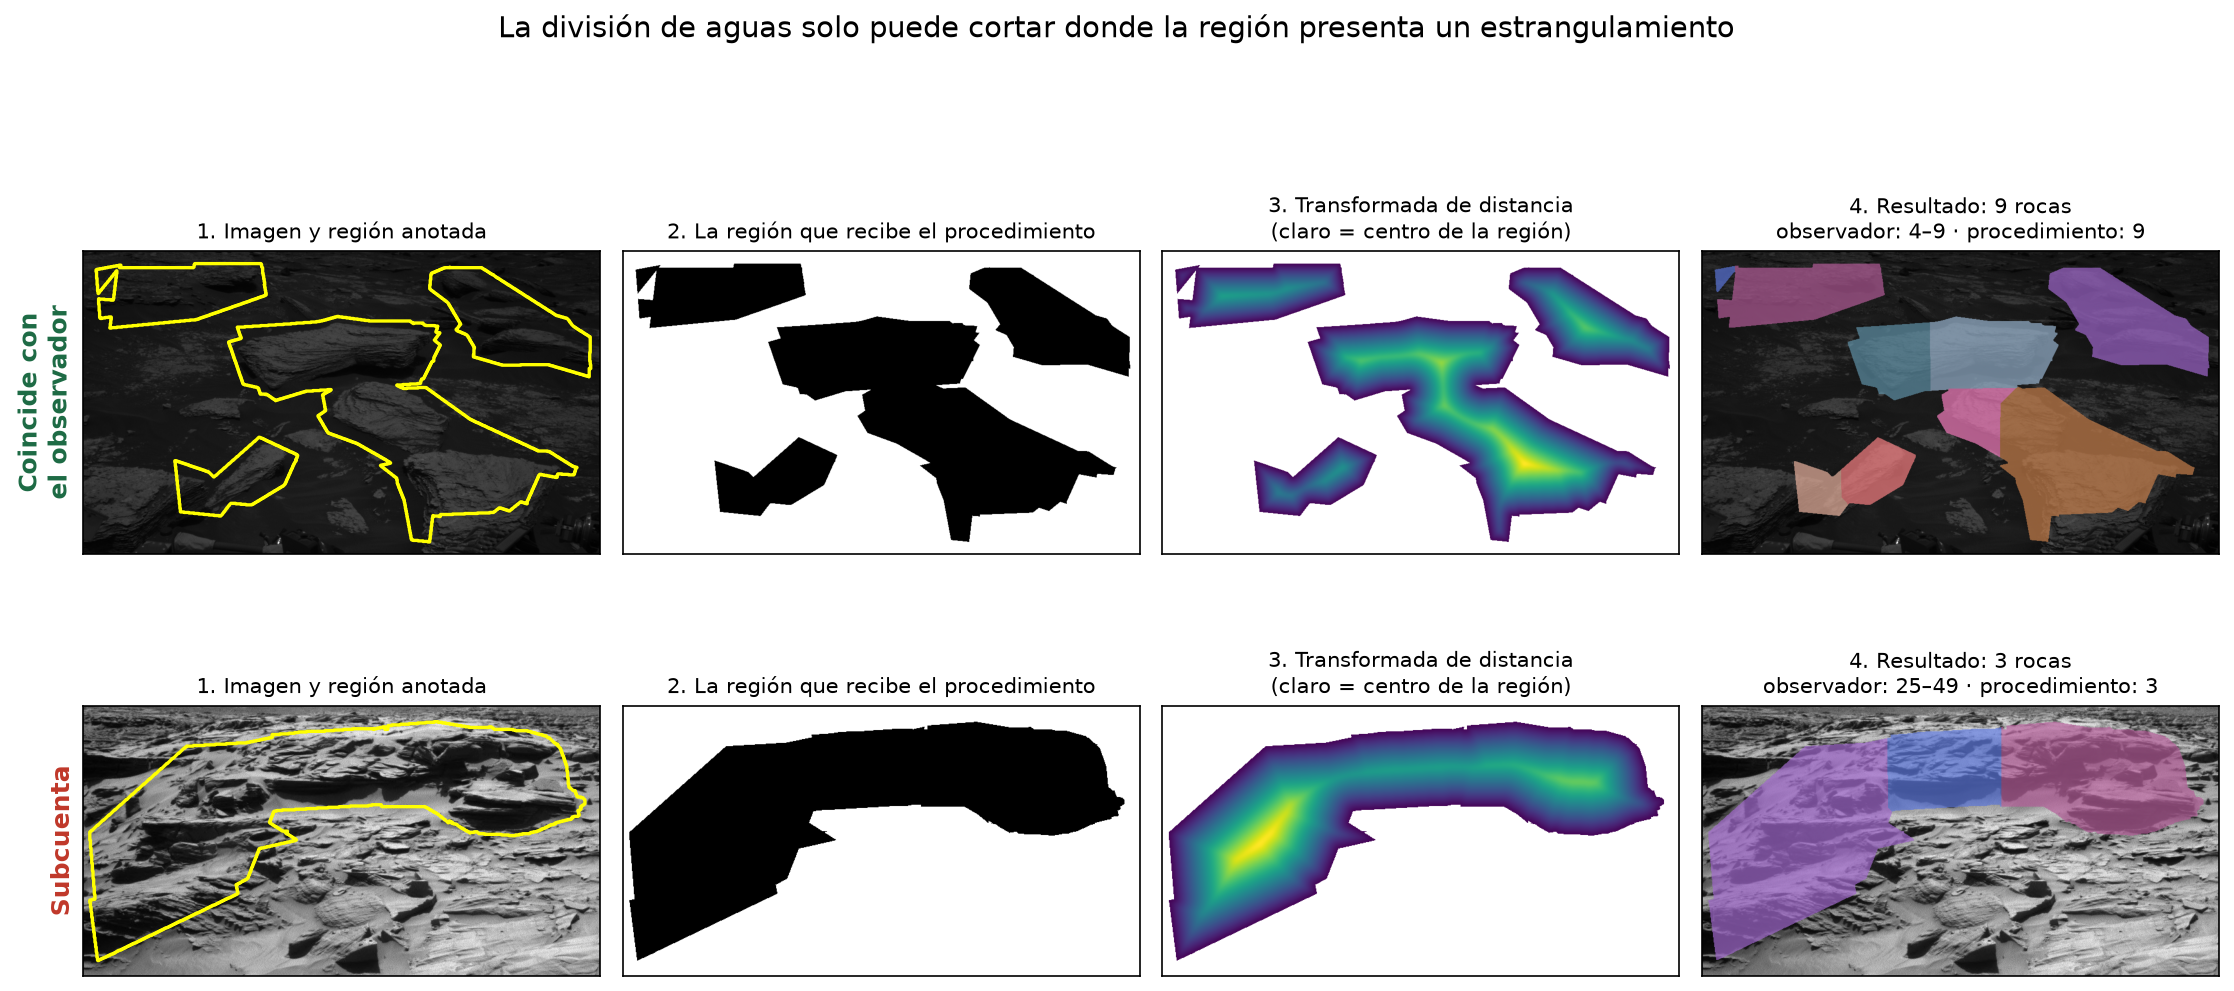
\includegraphics[width=\textwidth]{Figura_28_mecanismo_subconteo.png}
  \caption[Mecanismo del subconteo]{Arriba, una escena en la que la anotación delimita cada
    bloque por separado y el conteo coincide con el observador. Abajo, un único polígono
    envuelve un campo de bloques: la transformada de distancia no presenta estrangulamientos
    y la división de aguas no tiene dónde cortar.}
  \label{fig:mecanismo}
\end{figure}

\subsubsection{Alcance del indicador}

El procedimiento produce un conteo reproducible de las instancias geométricamente separables
dentro de la clase roca grande, pero ese conteo no puede interpretarse como estimación válida
del número total de rocas visibles en la escena. La evaluación exploratoria con un observador
sugiere un subconteo sistemático, atribuible tanto a la cobertura incompleta de la clase como a
regiones que no contienen la información geométrica necesaria para separar instancias.

Lo que el resultado sostiene es un uso más débil: ordenar de forma aproximada escenas según
contengan o no bloques discretos delimitados, sabiendo que el valor queda por debajo de lo que
un observador contaría. La conclusión debe moderarse además por el diseño de la validación: con
un único observador no es posible separar el desacuerdo entre algoritmo y persona de la
variabilidad natural entre personas, y la muestra, estratificada por área de la región, no es
representativa del subconjunto completo.

\subsection{Conteo con información de la imagen: exploración}
\label{sec:hibrido}

Si la máscara no contiene la información que separa los bloques, esa información solo puede
proceder de la imagen. Se exploró esa vía manteniendo el procedimiento clásico: la región
sigue siendo la que la anotación marcó como roca grande, pero el relieve sobre el que corta la
división de aguas se construye a partir de la imagen. Se compararon cuatro relieves: el
gradiente de intensidad a escala fina; el gradiente a escala gruesa, en el que la textura
interna se atenúa y persiste el borde; un realce de líneas oscuras finas mediante
\textit{top-hat} negro, que corresponde a las sombras entre rocas; y una combinación a partes
iguales de la geometría de la máscara y el gradiente. El protocolo es idéntico para los cuatro
—mismas semillas por prominencia y mismos filtros finales que E2—, y su único parámetro se
eligió por validación cruzada dejando una escena fuera, para que ninguna escena influyera en su
propio resultado. La diferencia con E2 se contrastó por \textit{bootstrap}, primero al
\SI{95}{\percent} y después con corrección de Bonferroni por el número de métodos probados
(Tabla~\ref{tab:metodos-imagen}).

\begin{table}[H]
  \centering
  \small
  \caption[Conteo con relieves derivados de la imagen]{Acuerdo con el observador de los
    conteos que usan la imagen dentro de la región anotada, frente al kappa ponderado de E2
    (\cVKappaPond).}
  \label{tab:metodos-imagen}
  \setlength{\tabcolsep}{4pt}
  \begin{tabular}{lccccc}
    \toprule
     & & & \multicolumn{3}{c}{\textbf{Diferencia de $\kappa$ ponderado con E2}} \\
    \cmidrule(lr){4-6}
    \textbf{Relieve} & \textbf{$\kappa$ pond.} & \textbf{Debajo / encima}
      & \textbf{Media} & \textbf{IC 95\,\%} & \textbf{IC Bonferroni} \\
    \midrule
    Gradiente fino     & \cMIGradKw    & \cMIGradAbajo{} / \cMIGradArriba       & \cMIGradDif    & \cMIGradIC    & \cMIGradICB \\
    Gradiente grueso   & \cMIPersistKw & \cMIPersistAbajo{} / \cMIPersistArriba & \cMIPersistDif & \cMIPersistIC & \cMIPersistICB \\
    Sombras            & \cMISombraKw  & \cMISombraAbajo{} / \cMISombraArriba   & \cMISombraDif  & \cMISombraIC  & \cMISombraICB \\
    Combinado          & \cMIComboKw   & \cMIComboAbajo{} / \cMIComboArriba     & \cMIComboDif   & \cMIComboIC   & \cMIComboICB \\
    \bottomrule
  \end{tabular}
\end{table}

Ningún relieve mejora a E2 de forma demostrable. El de sombras obtiene el mayor acuerdo y su
intervalo al \SI{95}{\percent} excluye el cero, pero deja de hacerlo al corregir por el número
de métodos probados. La sensibilidad lo confirma: sus \cMISombraVarN{} variantes de suavizado y
radio dan kappas ponderados entre \cMISombraVarMin{} y \cMISombraVarMax{}, y ninguna supera la
corrección de Bonferroni. Los cuatro relieves invierten además la dirección del error: todos
quedan por encima del observador en más escenas que por debajo —el de escala gruesa, en
\cMIPersistArriba{} de las \cVN—, lo que indica que cortan también en la textura interna de
las rocas y no solo en sus bordes. Corregir el subconteo con la imagen exige, por tanto,
controlar a la vez la sobresegmentación que la propia imagen introduce.

La Figura~\ref{fig:hibrido} ilustra el principio sobre la escena de la
Figura~\ref{fig:diag-bedrock}, etiquetada casi por completo como lecho rocoso y con conteo
nulo: el gradiente de la imagen, restringido a la región de roca de la máscara
(\cHibridoRegion{} de la escena), delimita \cHibridoN{} bloques cuyas fronteras siguen las
fracturas visibles. La cifra depende del umbral de prominencia de las semillas, es con toda
probabilidad un sobreconteo y no está validada.

\begin{figure}[H]
  \centering
  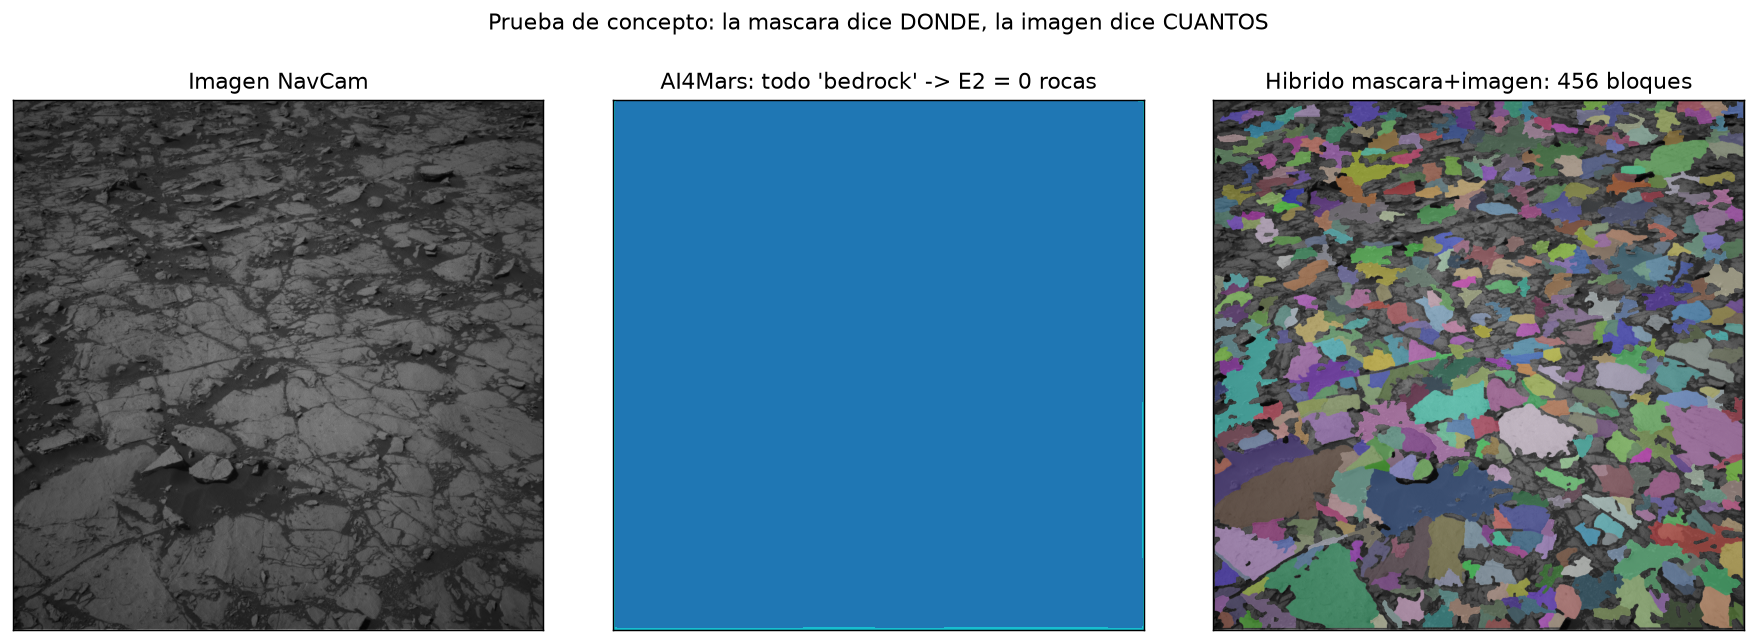
\includegraphics[width=\textwidth]{diag_prueba_hibrido.png}
  \caption[Prueba de concepto del enfoque híbrido]{Prueba de concepto: la máscara indica
    dónde hay roca y el gradiente de la imagen dónde están las fronteras entre bloques. El
    resultado ilustra el principio y no constituye un conteo validado.}
  \label{fig:hibrido}
\end{figure}

El enfoque híbrido se mantiene, por tanto, como \textbf{prueba de concepto}: muestra que la
imagen contiene información sobre las fronteras entre bloques que la máscara no recoge, pero
la evidencia reunida no permite concluir que la aproveche mejor que E2, y con \cVN{} escenas
y un solo observador la comparación carece de potencia para detectar mejoras moderadas. Su
evaluación con más observadores y una muestra independiente queda como trabajo futuro.

\subsection{Comparación con métodos de aprendizaje automático}

\paragraph{Modelo general sin entrenamiento específico.} El modelo fundacional de segmentación
\citep{kirillov2023sam}, en su variante rápida \citep{zhao2023fastsam}, se aplicó a \cSamN{}
imágenes con roca grande, restringiendo sus regiones a la zona etiquetada como roca. El acuerdo
con el conteo clásico, medido por bandas, es del \cSamAcuerdo, con correlación de rangos de
\cSamRho{} y un error absoluto medio de \cSamMAE{} rocas (Figura~\ref{fig:matriz-acuerdo}). El
modelo tiende a subdividir una misma roca según su textura interna y, en otras escenas, a no
detectar bloques de bajo contraste.

\begin{figure}[H]
  \centering
  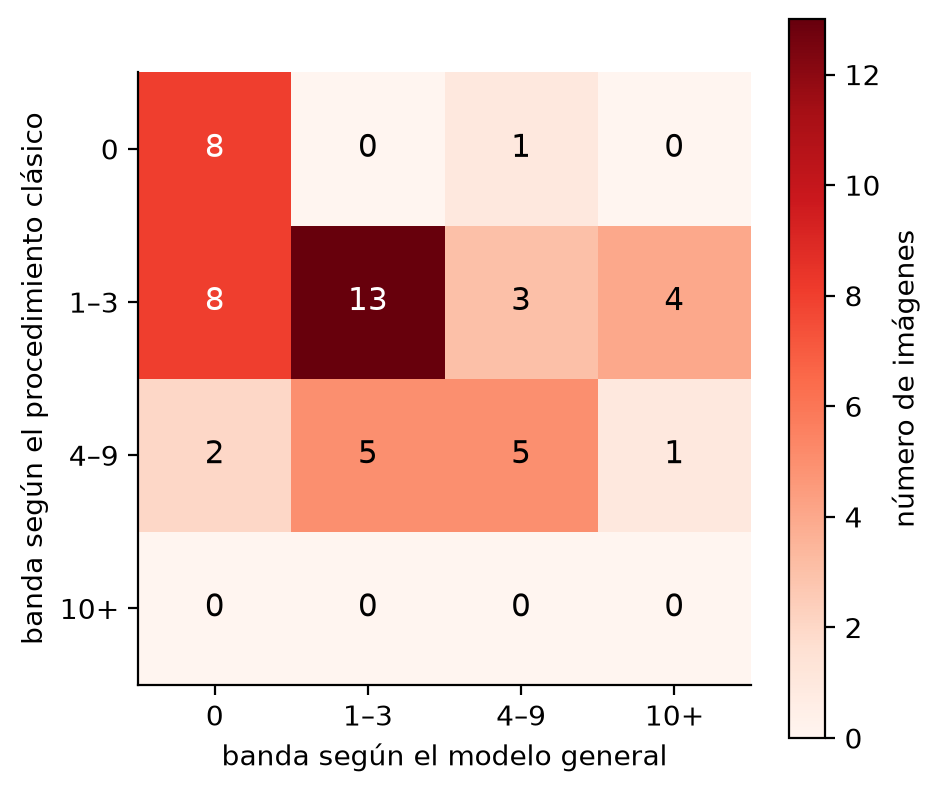
\includegraphics[width=0.72\textwidth]{Figura_20_matriz_acuerdo.png}
  \caption{Matriz de acuerdo entre el conteo clásico y el modelo general.}
  \label{fig:matriz-acuerdo}
\end{figure}

\paragraph{Segmentador entrenado con las propias máscaras.} El segmentador DeepLabV3, con la
configuración y el reparto por bloques temporales de la Tabla~\ref{tab:deeplab-config}, alcanzó
su mejor mIoU de validación en la época \cSegEpocaElegida{} (\cSegValMIoU, frente a
\cSegValUltima{} en la última), y ese es el modelo que se evaluó, una sola vez, sobre la prueba.
La Tabla~\ref{tab:deeplab} recoge su desempeño en tres conjuntos: la muestra equilibrada de
prueba, todas las escenas elegibles de los bloques de prueba con su distribución natural, y las
escenas de esos bloques que el umbral de fracción etiquetada había excluido.

\begin{table}[H]
  \centering
  \small
  \caption[Desempeño del segmentador entrenado]{Desempeño del segmentador sobre los bloques
    temporales de prueba, ninguno a menos de un sol de una imagen de entrenamiento. Error en
    puntos porcentuales; con signo, modelo menos etiqueta.}
  \label{tab:deeplab}
  \begin{tabular}{lccc}
    \toprule
     & \textbf{Muestra equilibrada} & \textbf{Distribución natural} & \textbf{Excluidas por fracción} \\
     & ($n = \cSegTest$) & ($n = \cSegNatN$) & ($n = \cSegExcN$) \\
    \midrule
    IoU de la clase no-roca       & \cSegIoUNo    & \cSegNatIoUNo    & \cSegExcIoUNo \\
    IoU de la clase roca          & \cSegIoURoca  & \cSegNatIoURoca  & \cSegExcIoURoca \\
    IoU medio                     & \textbf{\cSegMIoU} & \textbf{\cSegNatMIoU} & \cSegExcMIoU \\
    Correlación de la cobertura   & \cSegRCob     & \cSegNatR        & \cSegExcR \\
    Error absoluto medio          & \cSegMAE      & \cSegNatMAE      & \cSegExcMAE \\
    Error medio con signo         & \cSegErrMedio & \cSegNatErr      & \cSegExcErr \\
    \bottomrule
  \end{tabular}
\end{table}

El desempeño sobre la distribución natural es muy próximo al de la muestra equilibrada, de modo
que el equilibrio artificial de la prueba no infla las cifras. Las escenas con menos del
\SI{20}{\percent} de superficie etiquetada, en cambio, se segmentan claramente peor —error
absoluto medio de \cSegExcMAE{} puntos—: la exclusión no solo protege la función de pérdida,
también delimita el dominio en que el modelo es fiable.

\begin{figure}[H]
  \centering
  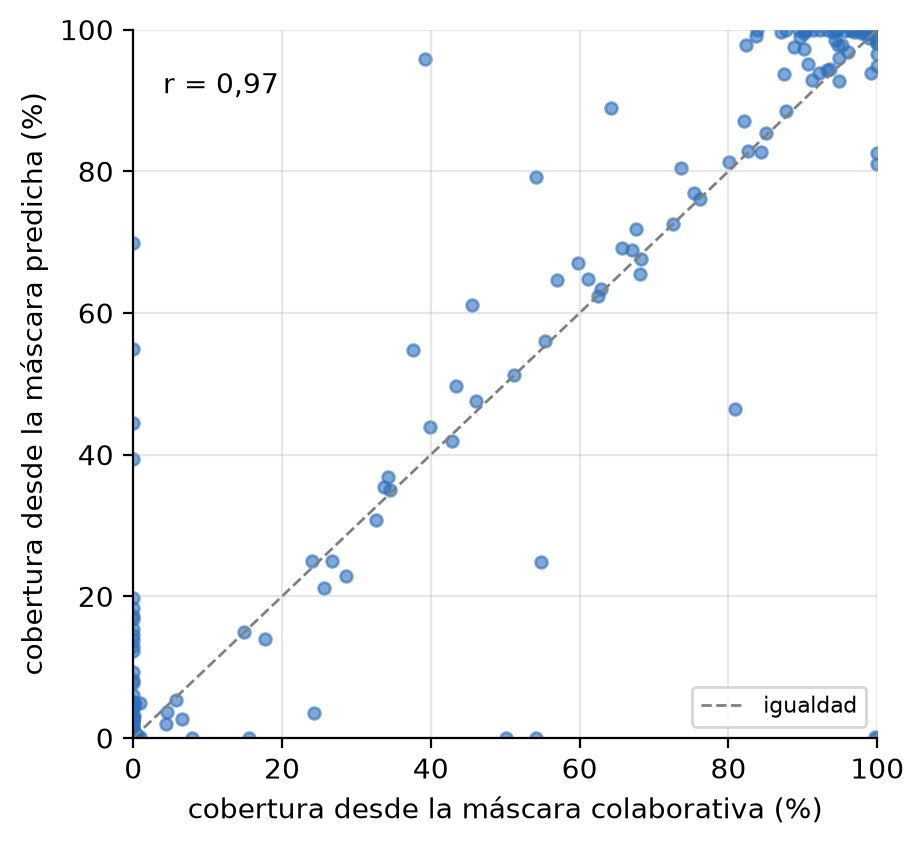
\includegraphics[width=0.62\textwidth]{Figura_21_cobertura_modelo_vs_humano.png}
  \caption[Cobertura del modelo frente a la humana]{Cobertura estimada por el modelo
    entrenado frente a la derivada de la anotación colaborativa, sobre las \cSegTest{}
    imágenes de la muestra equilibrada de prueba.}
  \label{fig:modelo-vs-humano}
\end{figure}

\paragraph{Fuga de información.} Con el reparto por bloques y el margen de un sol, la imagen de
prueba más próxima a una de entrenamiento está a \cFugaMinSoles{} soles, y la distancia mediana
es de \cFugaMedGapSoles{} soles. Una versión anterior del modelo, entrenada con un reparto al azar
por imagen, tenía \cAleMinuto{} imágenes de prueba (\cAleMinutoPct) a menos de un minuto de una
de entrenamiento, y obtenía un IoU medio de \cAleMIoU{} y una correlación de la cobertura de
\cAleR. Que el reparto por bloques entregue prácticamente las mismas cifras indica que aquella
proximidad no inflaba el desempeño. La Tabla~\ref{tab:fuga} muestra además que, dentro de la
prueba, el desempeño no depende de la distancia al entrenamiento.

\begin{table}[H]
  \centering
  \caption[Desempeño según la distancia temporal al entrenamiento]{Desempeño del segmentador
    sobre la muestra equilibrada de prueba según la distancia, en reloj de nave, de cada imagen
    a la imagen de entrenamiento más próxima.}
  \label{tab:fuga}
  \begin{tabular}{lrcc}
    \toprule
    \textbf{Distancia al entrenamiento} & \textbf{Imágenes} & \textbf{IoU medio}
      & \textbf{Correlación de la cobertura} \\
    \midrule
    De 1 a 10 soles     & \cFugaNA & \cFugaIoUA & \cFugaRA \\
    De 10 a 50 soles    & \cFugaNB & \cFugaIoUB & \cFugaRB \\
    Más de 50 soles     & \cFugaNC & \cFugaIoUC & \cFugaRC \\
    \bottomrule
  \end{tabular}
\end{table}

\subsubsection{Contraste del modelo con etiquetas de experto}
\label{sec:modelo-experto}

Se evaluó el mismo modelo, sin reentrenarlo, contra las \cNGold{} máscaras de experto,
restringiendo la comparación a los píxeles que el experto etiquetó. El IoU medio desciende a
\cExpMIoU{} (\cExpIoUNo{} en no-roca y \cExpIoURoca{} en roca) y la correlación de la cobertura
a \cExpR.

Una correlación alta no indica, por sí sola, ausencia de sesgo: mide si el orden de las escenas
se preserva, no si los valores coinciden. Para valorar el acuerdo se examinó el error con signo,
definido como la cobertura del modelo menos la de la etiqueta, tanto frente al experto como
frente a la muestra colaborativa aleatoria del apartado anterior
(Tabla~\ref{tab:modelo-experto}, Figuras~\ref{fig:modelo-experto}
y~\ref{fig:bland-altman}).

\begin{table}[H]
  \centering
  \caption[Error de la cobertura del modelo según la referencia]{Error de la cobertura del
    modelo según la referencia, en puntos porcentuales. Intervalos por \textit{bootstrap};
    límites de acuerdo de Bland--Altman como media $\pm\,1{,}96$ desviaciones típicas.}
  \label{tab:modelo-experto}
  \begin{tabular}{lcc}
    \toprule
    \textbf{Medida} & \textbf{Colaborativa} & \textbf{Experto} \\
     & ($n = \cBAColN$) & ($n = \cBAExpN$) \\
    \midrule
    Error medio, IC 95\,\%           & \cBAColMedia{} \cBAColMediaIC & \cBAExpMedia{} \cBAExpMediaIC \\
    Error mediano                    & \cBAColMediana & \cBAExpMediana \\
    Error absoluto medio, IC 95\,\%  & \cBAColMAE{} \cBAColMAEIC & \cBAExpMAE{} \cBAExpMAEIC \\
    Límites de acuerdo               & \cBAColLoA & \cBAExpLoA \\
    Escenas con error mayor de 10 p.p. & \cBAColDiez & \cBAExpDiez \\
    Escenas con error mayor de 50 p.p. & \cBAColCincuenta & \cBAExpCincuenta \\
    \bottomrule
  \end{tabular}
\end{table}

\begin{figure}[H]
  \centering
  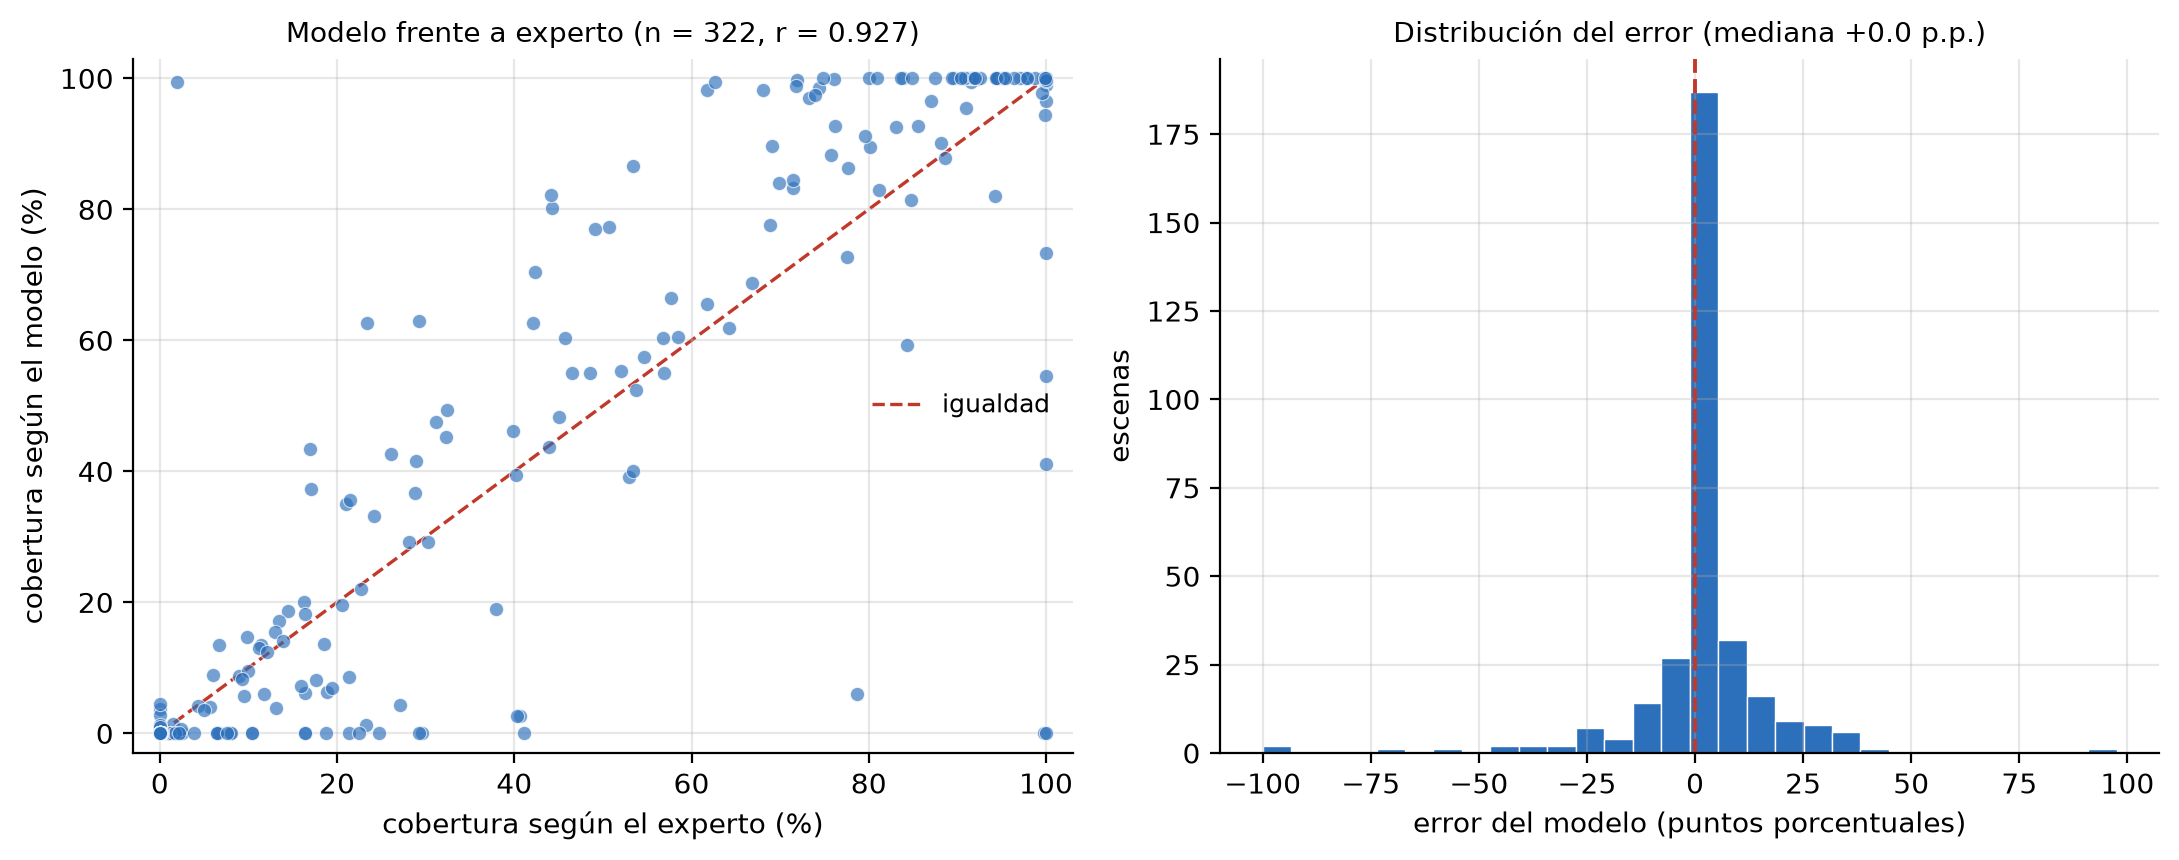
\includegraphics[width=\textwidth]{Figura_27_modelo_vs_experto.png}
  \caption[Cobertura del modelo frente a la del experto]{Cobertura estimada por el modelo
    frente a la derivada de la anotación de experto, y distribución del error con signo,
    sobre las \cNGold{} escenas con máscara de especialista.}
  \label{fig:modelo-experto}
\end{figure}

\begin{figure}[H]
  \centering
  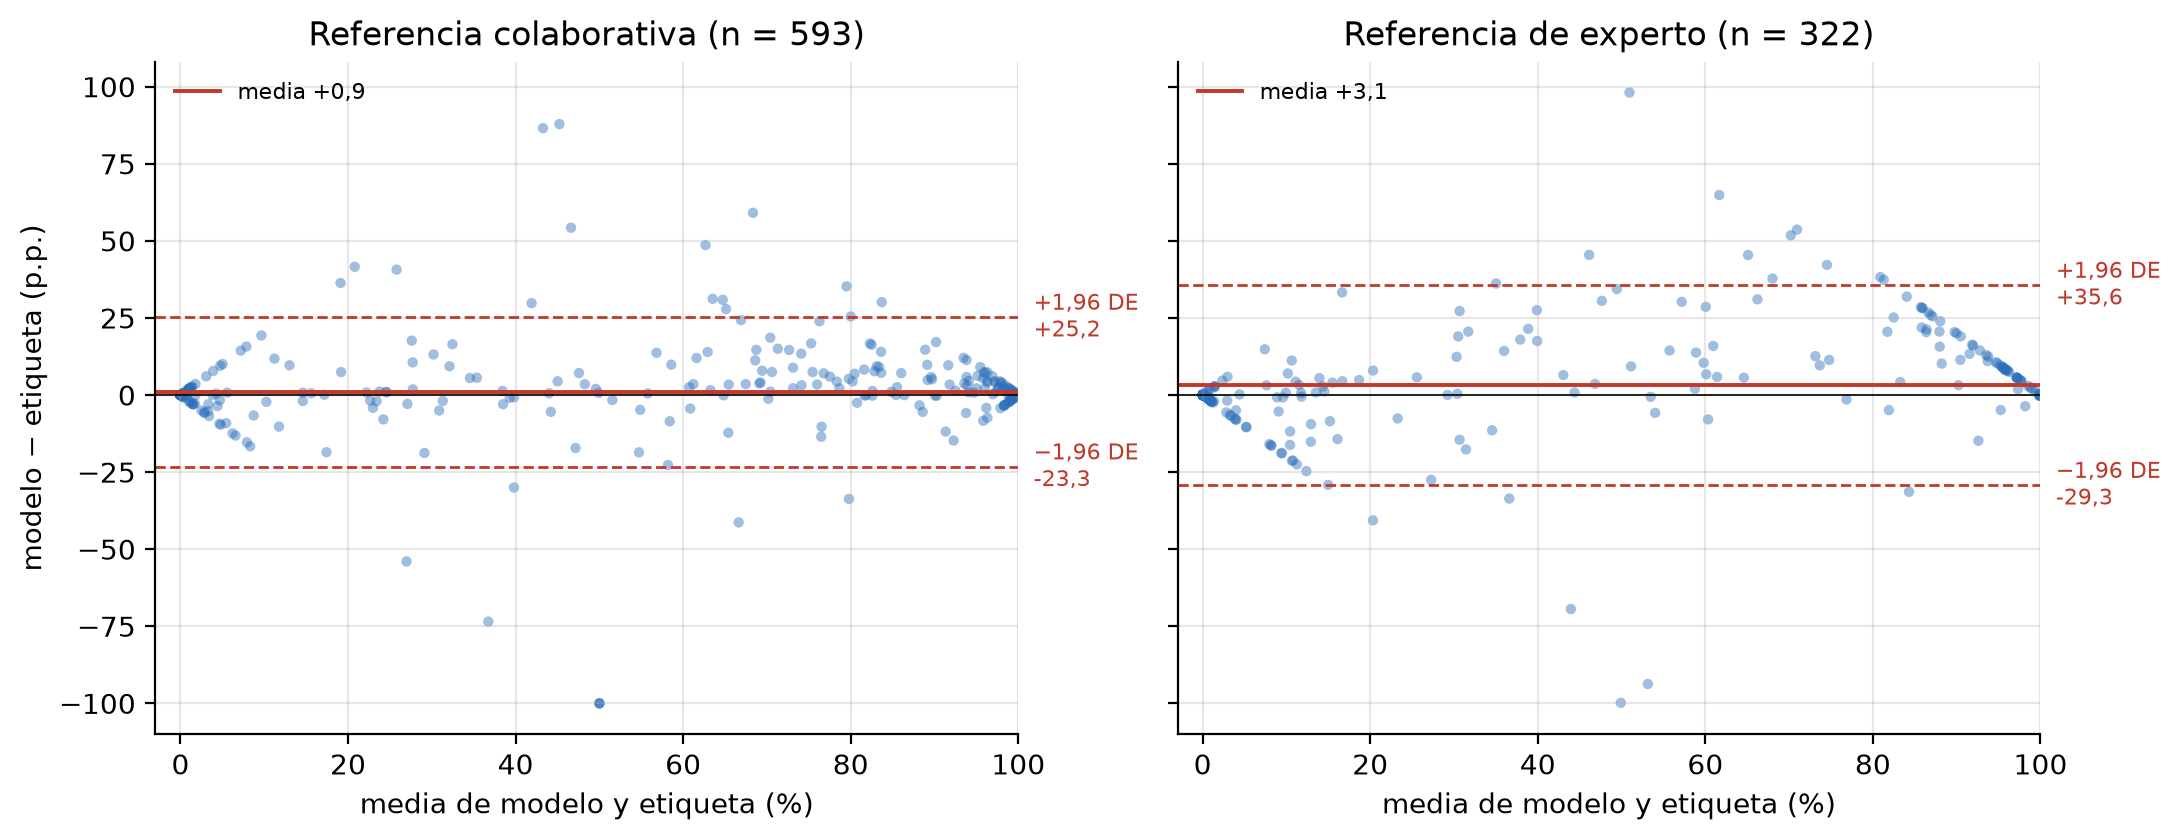
\includegraphics[width=\textwidth]{Figura_29_bland_altman.png}
  \caption[Diagrama de Bland--Altman]{Diferencia entre la cobertura del modelo y la de la
    etiqueta frente a su media, con la referencia colaborativa y con la de experto. Línea
    continua: error medio; discontinuas: límites de acuerdo.}
  \label{fig:bland-altman}
\end{figure}

Frente a la anotación colaborativa, el error medio es de \cBAColMedia{} puntos con un intervalo
que incluye el cero \cBAColMediaIC: en agregado, el modelo reproduce la referencia de la que
aprendió. Frente al experto, en cambio, \textbf{sobreestima}: el error medio es de
\cBAExpMedia{} puntos, con un intervalo que excluye el cero \cBAExpMediaIC{}, y el modelo queda
por encima del experto en más escenas que por debajo. Ninguna de las dos cifras autoriza a
llamar al modelo insesgado, y la mediana nula no lo contradice: refleja que en el \cExpExactas{}
de las escenas modelo y etiqueta coinciden exactamente, casi siempre porque ninguno de los dos
encuentra roca. El error absoluto medio frente al experto es de \cBAExpMAE{} puntos, los límites
de acuerdo abarcan unos sesenta y cinco puntos porcentuales y el \cBAExpDiez{} de las escenas
supera los diez puntos de error.

El error tampoco es homogéneo (Tabla~\ref{tab:error-tramos}). Frente al experto, la
sobreestimación se concentra en las coberturas intermedias —entre el \SI{25}{\percent} y el
\SI{75}{\percent} el error medio supera los diez puntos— y se invierte en las escenas de
cobertura total; por tipo de escena, el error es pequeño en las de suelo y mayor en las mixtas.
Un error medio moderado resulta, en parte, de errores de signo opuesto en distintos tramos que
se compensan.

\begin{table}[H]
  \centering
  \small
  \caption[Error del modelo por tramo de cobertura y tipo de escena]{Error de la cobertura
    del modelo por tramo de cobertura de la referencia y por tipo de escena: número de
    escenas, error medio con signo y error absoluto medio, en puntos porcentuales.}
  \label{tab:error-tramos}
  % ARCHIVO GENERADO por scripts/generar_cifras.py — no editar a mano.
\begin{tabular}{lrrrrrr}
\toprule
 & \multicolumn{3}{c}{\textbf{Referencia colaborativa}} & \multicolumn{3}{c}{\textbf{Referencia de experto}} \\
\cmidrule(lr){2-4}\cmidrule(lr){5-7}
 & $n$ & Medio & Absoluto & $n$ & Medio & Absoluto \\
\midrule
\multicolumn{7}{l}{\textit{Por tramo de cobertura de la referencia (\%)}} \\
0 & 171 & \ensuremath{+}\num{1.3} & \num{1.3} & 108 & \ensuremath{+}\num{0.6} & \num{0.6} \\
0--25 & 68 & \ensuremath{+}\num{2.2} & \num{7.2} & 82 & \num{-0.3} & \num{8.3} \\
25--50 & 28 & \ensuremath{+}\num{6.6} & \num{11.6} & 28 & \ensuremath{+}\num{13.0} & \num{23.6} \\
50--75 & 49 & \ensuremath{+}\num{3.4} & \num{13.6} & 28 & \ensuremath{+}\num{16.3} & \num{19.8} \\
75--99,99 & 97 & \ensuremath{+}\num{1.7} & \num{4.8} & 55 & \ensuremath{+}\num{5.1} & \num{11.7} \\
100 & 180 & \num{-1.9} & \num{1.9} & 21 & \num{-6.9} & \num{6.9} \\
\midrule
\multicolumn{7}{l}{\textit{Por tipo de escena}} \\
Suelo & 200 & \ensuremath{+}\num{1.3} & \num{2.9} & 142 & \num{-1.5} & \num{3.7} \\
Arenoso & 64 & \ensuremath{+}\num{5.1} & \num{7.0} & 69 & \ensuremath{+}\num{6.1} & \num{9.5} \\
Rocoso & 298 & \num{-0.4} & \num{3.7} & 89 & \ensuremath{+}\num{4.9} & \num{12.2} \\
Mixto & 31 & \ensuremath{+}\num{2.7} & \num{13.1} & 22 & \ensuremath{+}\num{16.5} & \num{22.3} \\
\bottomrule
\end{tabular}

\end{table}

\paragraph{Lectura.} El segmentador estima la cobertura con un desempeño alto frente a la
anotación de la que aprendió y algo menor frente al experto, respecto del cual sobreestima unos
tres puntos de media, con errores individuales grandes y dependientes del tramo. Esa
sobreestimación es la esperable si el modelo heredó el criterio de la anotación colaborativa. Sirve, por tanto, para describir conjuntos de escenas y no para valorar una escena
concreta. Estima cobertura, no conteo: distingue roca de no-roca y no separa bloques, de modo
que no sustituye a E2. Con esas reservas, que la imagen sola permita aproximar la cobertura
sugiere que el indicador podría calcularse sin anotación humana, posibilidad que el
Capítulo~\ref{cap:conclusiones} recoge como línea futura.

\section{Implicaciones y limitaciones}

\subsection{Contraste de las hipótesis}

La Tabla~\ref{tab:contraste-hipotesis} resume el contraste de las hipótesis de la
Sección~\ref{sec:hipotesis} con la evidencia de este capítulo.

\begin{table}[H]
  \centering
  \small
  \caption{Contraste de las hipótesis de trabajo.}
  \label{tab:contraste-hipotesis}
  \begin{tabular}{p{1.0cm}p{8.6cm}p{3.6cm}}
    \toprule
    \textbf{Hip.} & \textbf{Evidencia} & \textbf{Dictamen} \\
    \midrule
    H1 & El cálculo es determinista y reproducible. Sin asociación lineal con la fracción
      etiquetada ($r = \cDepFCPearson$); dependencia no lineal débil pero detectable
      (correlación de distancia \cDepFCDcor); la cobertura por tramos de fracción no sigue el
      patrón que produciría el artefacto del denominador.
      & Se sostiene, con dependencia residual débil \\
    H2 & Kappa ponderado \cVKappaPond{} \cVKappaPondIC; \cVAbajo{} escenas por debajo del
      observador y \cVArriba{} por encima; subconteo en las \cSenN{} combinaciones de
      parámetros.
      & Se rechaza, en una evaluación exploratoria \\
    H3 & Diferencia de medianas de \cFuenteDifMed{} puntos entre fuentes. El instrumento común
      atribuye el \cDescImgPct{} de la diferencia de medias a las imágenes y \cDescAnot{}
      puntos \cDescAnotIC{} a la anotación.
      & Se rechaza: hay efecto de la fuente, menor que la diferencia bruta \\
    H4 & Sin asociación lineal ni monótona ($r = \cDepCCPearson$, $\rho = \cDepCCSpearman$);
      dependencia no lineal débil (correlación de distancia \cDepCCDcor, $p = \cDepCCDcorP$)
      en forma de U invertida; los deciles de cobertura explican el \cEtaConteo{} de la
      varianza del conteo.
      & Se sostiene: información distinta, no independencia \\
    \bottomrule
  \end{tabular}
\end{table}

\subsection{Interpretación de los indicadores}

El trabajo confirma que las máscaras de AI4Mars pueden leerse como mapas cuantitativos y no
solo como insumo de entrenamiento, con límites distintos para cada indicador.

La cobertura es el indicador sólido. Se calcula para el \cPctCobCalc{} de las escenas, es
reproducible y no está gobernada por la fracción de escena etiquetada. Su valor, sin embargo,
depende de quién anotó: aplicada a máscaras de experto produciría coberturas algo menores, y
la comparación directa con esas máscaras está dominada por el hecho de que cubren escenas
mucho menos rocosas. Las coberturas reportadas describen, por tanto, el terreno tal como lo
registra la anotación colaborativa, y son adecuadas para comparar escenas del mismo conjunto.

El conteo es el indicador limitado. Cuenta de forma reproducible las instancias que la
geometría de la máscara permite separar, pero no el número de rocas que un observador
distingue. Cobertura y conteo aportan información distinta —conocer uno informa muy poco sobre
el otro—, de modo que reportarlos por separado está justificado, aunque no sean
estadísticamente independientes.

\subsection{Diagnóstico de los modos de error del conteo}
\label{sec:diagnostico}

Al inspeccionar visualmente los resultados se observaron dos comportamientos opuestos:
escenas en las que el conteo señalaba rocas donde un observador no las percibía, y escenas con
bloques evidentes en las que el conteo era nulo. Puesto que una explicación natural sería la
insuficiencia de las imágenes, se hizo un diagnóstico sistemático para atribuir cada modo de
error a su causa.

La primera constatación es de orden metodológico: \textbf{el procedimiento no lee las
imágenes}, sino las máscaras, de modo que su calidad no interviene directamente en el conteo.
Las imágenes son además de \num{1024}$\times$\num{1024} píxeles, resolución completa de la
cámara, y las máscaras tienen exactamente el mismo tamaño, por lo que tampoco hay pérdida por
remuestreo.

La Tabla~\ref{tab:diagnostico} reparte las \cNEscenas{} escenas según el resultado del
conteo.

\begin{table}[H]
  \centering
  \caption{Reparto de las escenas según el resultado del conteo.}
  \label{tab:diagnostico}
  \small
  \begin{tabular}{lrrl}
    \toprule
    \textbf{Situación} & \textbf{Escenas} & \textbf{\%} & \textbf{Naturaleza} \\
    \midrule
    La máscara no tiene ningún píxel de roca grande & \cNSinBig     & \cPctSinBig    & límite de la etiqueta \\
    Roca grande en escena casi sin etiquetar (excluida) & \cNNullBig & \cPctNullBig & población de E2 \\
    Roca grande, pero los filtros la descartan       & \cNFiltradas  & \cPctFiltradas & límite de los umbrales \\
    Al menos una roca contada                        & \cNConRocas   & \cPctConRocas  & --- \\
    \bottomrule
  \end{tabular}
\end{table}

El primer grupo es con mucho el mayor, y su componente principal son las \cFlagNoBig{} escenas
con bandera \texttt{no\_bigrock}: \textbf{hay roca visible, pero el anotador la etiquetó como
lecho rocoso}. La mediana de lecho rocoso en ese grupo es del \cNoBigBedMed, y
\cNoBigBedOchenta{} escenas tienen más del \SI{80}{\percent} de lecho rocoso y ninguna roca
grande. El desequilibrio es estructural: sobre las escenas con roca, el lecho rocoso aporta el
\cParteBed{} de la roca etiquetada y la roca grande solo el \cParteBig, y E2 cuenta únicamente
esta última.

La Figura~\ref{fig:diag-bedrock} muestra el caso con claridad: una escena con bloques
individuales distinguibles, etiquetada en su totalidad como lecho rocoso, sobre la que el
conteo devuelve cero.

\begin{figure}[H]
  \centering
  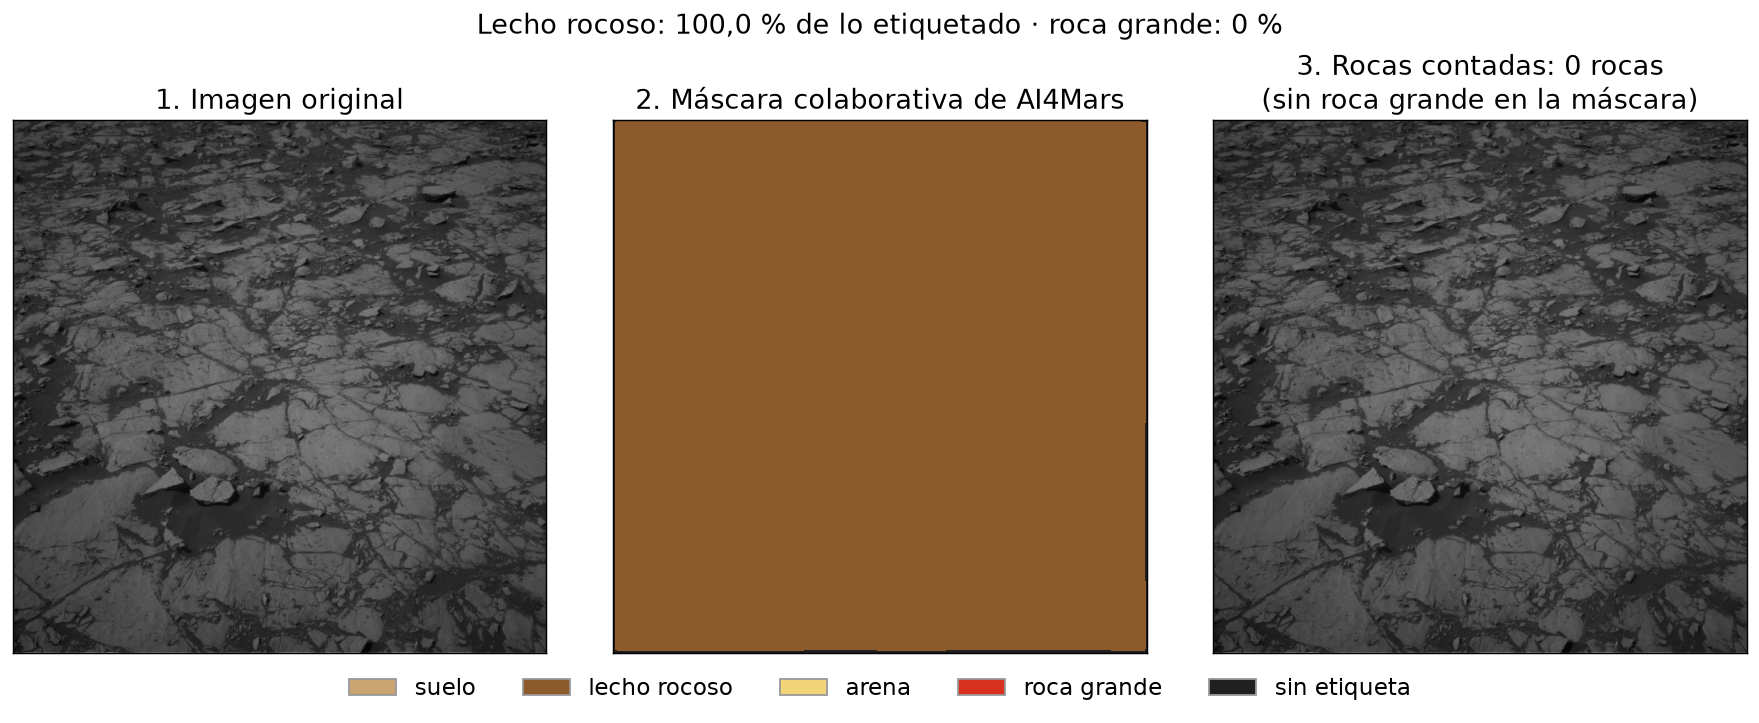
\includegraphics[width=\textwidth]{diag_bedrock_no_contado.png}
  \caption[Roca visible etiquetada como lecho rocoso]{Escena con bloques individuales
    evidentes, etiquetada íntegramente como lecho rocoso. El conteo devuelve cero porque
    la clase roca grande no está presente en la máscara.}
  \label{fig:diag-bedrock}
\end{figure}

El grupo de escenas cuyos píxeles de roca grande descartan los filtros —\cNFiltradas, el
\cPctFiltradas{} del conjunto— se revisó y los filtros \textbf{cumplen su función}: se trata de
motas de pocos píxeles, con un ejemplo de una única región de doce píxeles frente al umbral de
\num{524}, o de bandas muy alargadas trazadas sobre el horizonte, descartadas por relación de
aspecto (Anexo~\ref{app:material-complementario}). No se encontraron motivos para relajar los
umbrales.

Por el lado del conteo excesivo, la Tabla~\ref{tab:falsos-positivos} recoge las tres fuentes
identificadas.

\begin{table}[H]
  \centering
  \caption{Fuentes de conteo excesivo.}
  \label{tab:falsos-positivos}
  \begin{tabular}{lrl}
    \toprule
    \textbf{Fuente} & \textbf{Magnitud} & \textbf{Naturaleza} \\
    \midrule
    Subdivisión por división de aguas & \cNSubdiv{} de \cNConRocas{} escenas & algoritmo \\
    Artefacto de anotación            & \cNArtefacto{} escenas, todas excluidas de E2 & etiqueta \\
    Anotación en contorno hueco       & 1 de \num{1019} regiones examinadas & anecdótico \\
    \bottomrule
  \end{tabular}
\end{table}

La subdivisión afecta al \cPctSubdiv{} de las escenas que cuentan alguna roca —aquellas en que
el número de rocas supera el de componentes conectadas— y esas escenas aportan \cRocasSubdiv{}
de las \cNRocas{} rocas, de modo que es la limitación algorítmica cuantitativamente más
importante. No toda subdivisión es un error, porque separar rocas unidas es precisamente la
función de la división de aguas; la Figura~\ref{fig:subdivision} ilustra el caso en que sí lo
es, sobre un afloramiento continuo.

\begin{figure}[H]
  \centering
  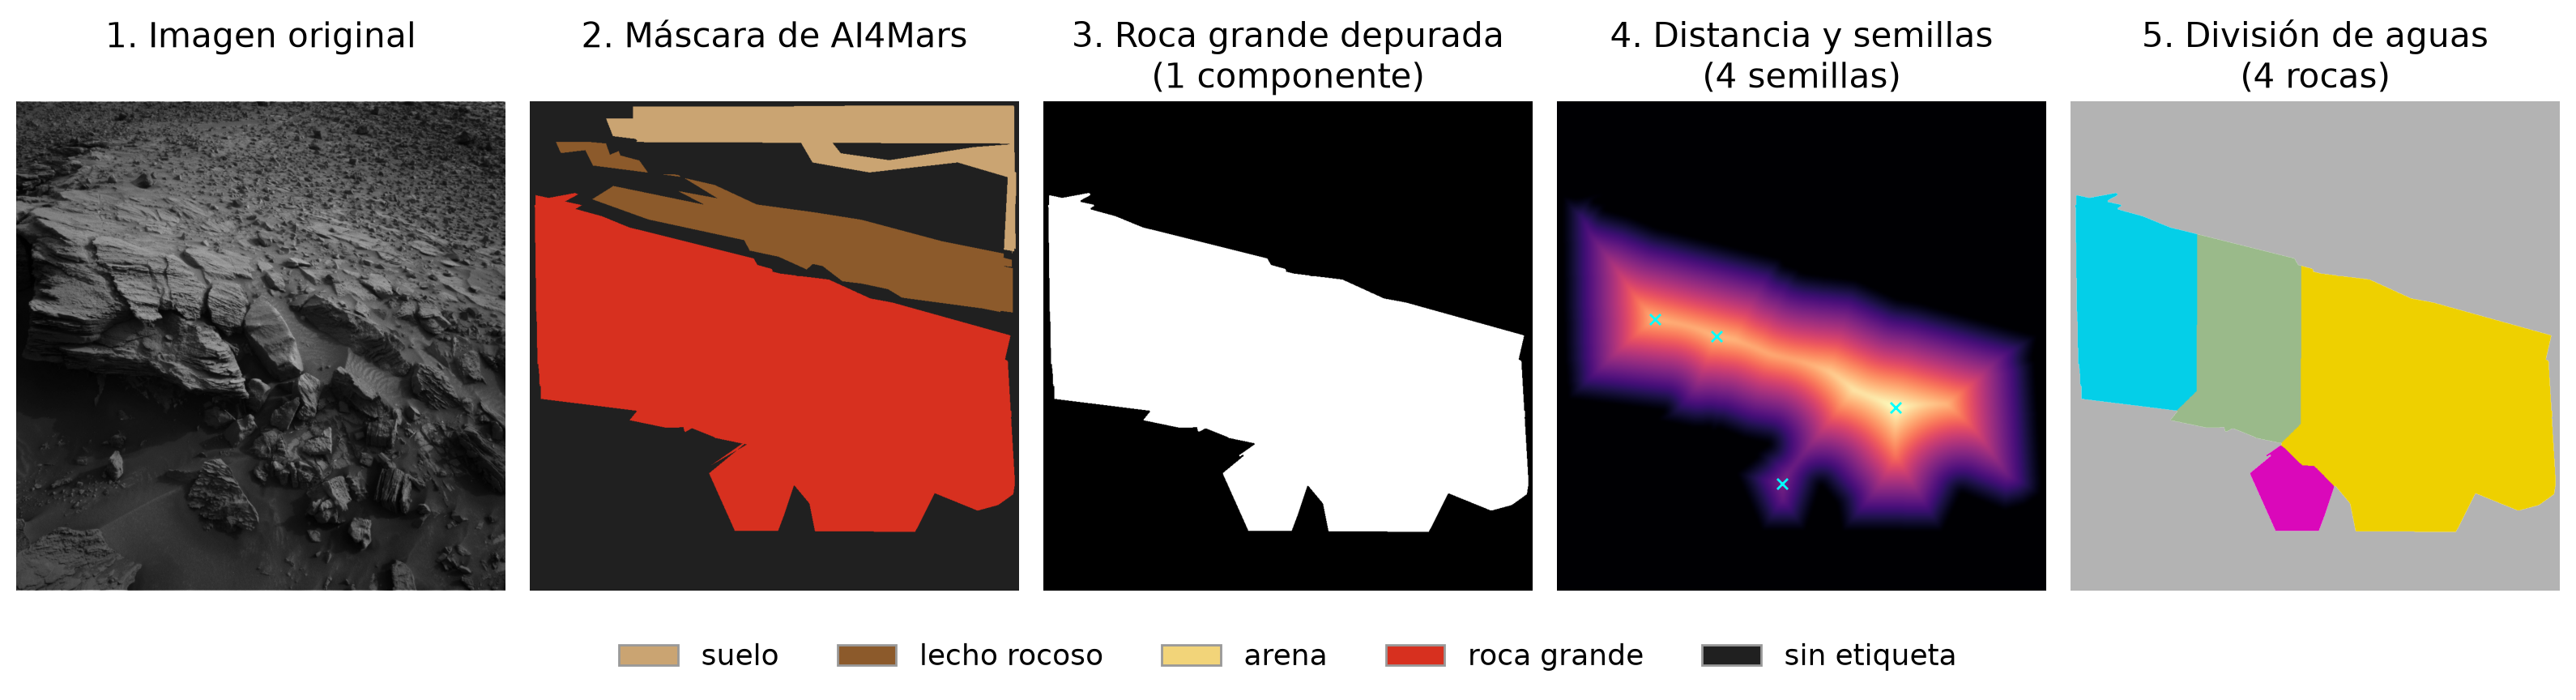
\includegraphics[width=0.9\textwidth]{Figura_22_subdivision_afloramiento.png}
  \caption{Subdivisión de un afloramiento continuo por la división de aguas.}
  \label{fig:subdivision}
\end{figure}

Los artefactos de anotación —escenas con menos del \SI{5}{\percent} de superficie etiquetada en
las que la roca mayor ocupa casi toda el área válida— son el falso positivo más llamativo. La
Figura~\ref{fig:diag-artefacto} muestra un ejemplo. Las \cNArtefacto{} escenas que cumplen ese
criterio tienen bandera \texttt{mostly\_null} y quedan fuera de la población de E2; dentro de
ella hay \cNArtefactoOk. Es la razón principal para excluir esa bandera del conteo.

\begin{figure}[H]
  \centering
  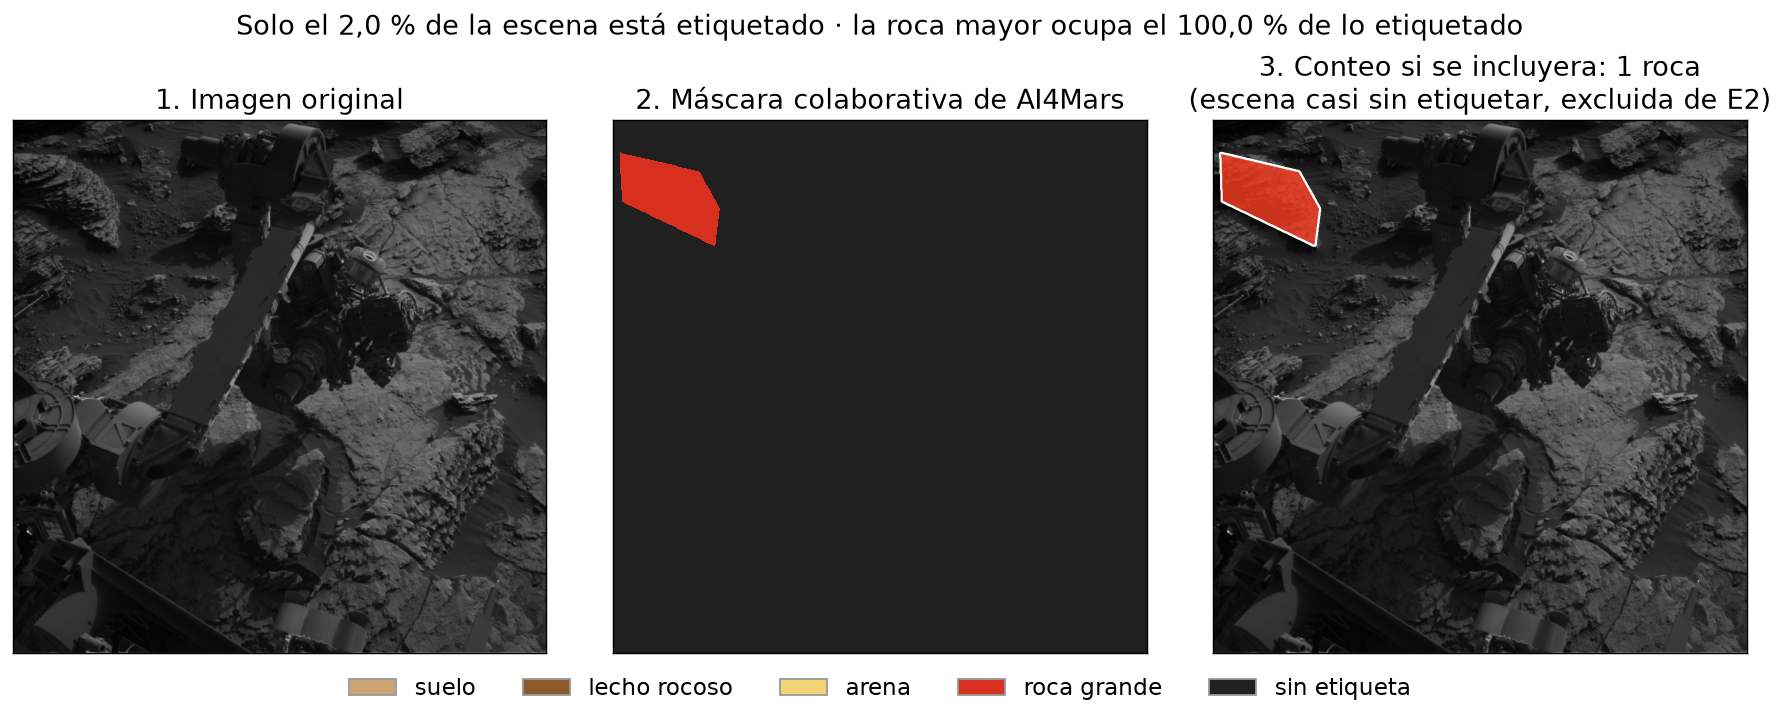
\includegraphics[width=\textwidth]{diag_artefacto_anotacion.png}
  \caption[Artefacto de anotación]{Escena con solo el \SI{2.0}{\percent} de los píxeles
    etiquetados, marcados en su totalidad como roca grande. Tiene bandera
    \texttt{mostly\_null} y no forma parte de la población de E2.}
  \label{fig:diag-artefacto}
\end{figure}

La anotación en forma de contorno hueco se midió sobre una muestra de \num{600} escenas con
roca grande y resultó \textbf{rara}: una región de las \num{1019} examinadas. Se reporta por
completitud, pero no justifica un filtro adicional.

\subsection{El límite del conteo: representación semántica y granularidad}
\label{sec:limite-conteo}

Un contraste adicional completa el diagnóstico. Los tres conjuntos de máscaras de experto que
el propio AI4Mars incluye corresponden a las \textbf{mismas} \cNGold{} imágenes con exigencias
de acuerdo crecientes entre especialistas. La proporción de escenas con roca grande disminuye
a medida que se exige mayor acuerdo (Tabla~\ref{tab:gold}).

\begin{table}[H]
  \centering
  \caption[Presencia de roca grande según la fuente de etiqueta]{Presencia de roca grande
    según la fuente de etiqueta y el nivel de acuerdo exigido. La cobertura mediana se
    calcula aquí sobre todas las escenas del conjunto —no solo sobre las que contienen
    roca—, por lo que difiere de la reportada en la Tabla~\ref{tab:validacion}.}
  \label{tab:gold}
  \begin{tabular}{lrrrr}
    \toprule
    \textbf{Fuente} & \textbf{Escenas} & \textbf{Con roca grande} & \textbf{Conteo medio}
    & \textbf{Cobertura mediana} \\
    \midrule
    Colaborativas       & \cNEscenas & \cPctBigAny  & \cColabRocas    & \cColabCobMed \\
    Experto, nivel 1    & \cNGold    & \cGoldUnoBig  & \cGoldUnoRocas  & \cGoldUnoCobMed \\
    Experto, nivel 2    & \cNGold    & \cGoldDosBig  & \cGoldDosRocas  & \cGoldDosCobMed \\
    Experto, nivel 3    & \cNGold    & \cGoldTresBig & \cGoldTresRocas & \cGoldTresCobMed \\
    \bottomrule
  \end{tabular}
\end{table}

Como las imágenes son las mismas en los tres niveles, la caída no puede deberse a diferencias de
terreno: indica que los especialistas discrepan sobre qué píxeles son roca grande, y que esos
píxeles desaparecen al exigir consenso. La frontera entre roca grande y lecho rocoso es, por
tanto, ambigua también para los expertos.

La evidencia indica que la principal limitación observada para el conteo de instancias proviene
de la representación semántica y de la granularidad de las etiquetas, más que de una falta de
resolución evidente de las imágenes. Una máscara de clases no distingue instancias; la clase
lecho rocoso absorbe la mayoría de los bloques que un observador contaría, y cuando la clase
roca grande aparece, a menudo agrupa varios bloques en un solo polígono. No es posible, con
todo, aislar la taxonomía como causa única. Intervienen también las reglas de agregación y de
consenso con que se fusionan las anotaciones, la perspectiva y la escala variable de una
cámara de navegación, la oclusión entre bloques y la propia parametrización del procedimiento.

\subsection{Síntesis: por qué contar rocas con estas máscaras no es sencillo}
\label{sec:sintesis-conteo}

El resultado negativo del conteo no procede de un único fallo, sino de varios obstáculos que se
superponen y que ningún ajuste del procedimiento resuelve por sí solo:

\begin{enumerate}
  \item \textbf{La clase que se cuenta es minoritaria.} La roca grande aporta el \cParteBig{} de
    la roca etiquetada; el resto, incluidos muchos bloques que un observador contaría, se anotó
    como lecho rocoso y queda fuera del conteo por definición.
  \item \textbf{La anotación de esa clase no es exhaustiva.} En \cVNoExhN{} de las \cVN{}
    escenas de la validación, la roca grande es menos del \SI{20}{\percent} de la roca
    etiquetada: se marcaron algunas rocas, no todas.
  \item \textbf{La geometría de la máscara no siempre separa instancias.} Cuando un polígono
    envuelve un campo de bloques contiguos, no hay estrangulamientos por donde cortar, y la
    información que separaría los bloques está en la imagen, no en la máscara.
  \item \textbf{La calibración enfrenta un dilema.} Contener la sobresegmentación de las losas
    continuas exige un criterio de semillas más estricto, y ese criterio rebajó el conteo de
    forma general (Sección~\ref{sec:calibracion}). Ninguna de las \cSenN{} combinaciones de
    parámetros ensayadas elimina el subconteo.
  \item \textbf{Usar la imagen no lo resuelve de forma demostrable.} Los relieves derivados de la
    imagen corrigen la dirección del error pero tienden a sobreestimar, y ninguno mejora el
    acuerdo con el observador una vez corregido el número de métodos probados.
\end{enumerate}

\subsection{Síntesis: inconsistencias del conjunto de datos}
\label{sec:inconsistencias}

El examen de las máscaras reveló además varias inconsistencias en el propio conjunto de datos,
que condicionan cualquier indicador derivado de él y cualquier evaluación que lo tome como
referencia. La Tabla~\ref{tab:inconsistencias} las reúne con su evidencia y su consecuencia.

\begin{table}[H]
  \centering
  \small
  \caption[Inconsistencias del conjunto de datos]{Inconsistencias del conjunto de datos AI4Mars
    (cámara de navegación de \textit{Curiosity}) identificadas en este trabajo.}
  \label{tab:inconsistencias}
  \begin{tabular}{p{3.6cm}p{5.4cm}p{5.0cm}}
    \toprule
    \textbf{Inconsistencia} & \textbf{Evidencia} & \textbf{Consecuencia} \\
    \midrule
    Composición distinta entre las escenas de entrenamiento y las de especialista
      & Medida por un mismo instrumento, cobertura mediana del \cFARegMedExp{} frente al
        \cFARegMedColab; el \cDescImgPct{} de la diferencia entre fuentes procede de las
        imágenes (Sección~\ref{sec:experto})
      & Una caída de desempeño al pasar de un conjunto al otro mezcla el cambio de anotación
        con el de terreno \\
    Criterio de anotación distinto entre voluntarios y especialistas
      & Componente de anotación de \cDescAnot{} puntos \cDescAnotIC, entre dos y cuatro según el
        instrumento
      & Las coberturas son relativas a la fuente que anotó \\
    Frontera ambigua entre roca grande y lecho rocoso
      & Sobre las mismas \cNGold{} imágenes, las escenas con roca grande pasan del
        \cGoldUnoBig{} al \cGoldTresBig{} al exigir acuerdo entre especialistas
        (Sección~\ref{sec:limite-conteo})
      & El conteo depende de qué se decidió llamar roca grande \\
    Anotación no exhaustiva de la roca grande
      & En \cVNoExhN{} de \cVN{} escenas, menos del \SI{20}{\percent} de la roca etiquetada;
        mediana del \cVNoExhMed{} (Sección~\ref{sec:anotacion-parcial})
      & El conteo no puede estimar las rocas presentes \\
    Granularidad variable del trazado
      & Polígonos que delimitan cada bloque junto a polígonos que envuelven campos enteros
        (Figura~\ref{fig:mecanismo})
      & El mismo procedimiento acierta o subcuenta según cómo se trazó \\
    Escenas casi sin etiquetar
      & \cFlagNull{} escenas con más del \SI{95}{\percent} sin etiqueta; \cNNullBig{} con roca
        grande, entre ellas los artefactos de anotación
      & Deben excluirse del conteo \\
    \bottomrule
  \end{tabular}
\end{table}

Ninguna de estas inconsistencias invalida el conjunto para el propósito con que se creó
—entrenar segmentadores de terreno para la navegación—, pero todas limitan su uso como medida
cuantitativa del terreno y como referencia de evaluación. Documentarlas es, a juicio de este
trabajo, su aporte más transferible.

\subsection{Limitaciones}

Además de las señaladas en cada apartado, conviene reunir las principales.

\paragraph{Ausencia de escala métrica.} Los tamaños son relativos al campo de visión. Sin la
geometría de la cámara o la información estereoscópica no es posible expresarlos en
centímetros ni construir distribuciones tamaño--frecuencia comparables en magnitud con la
literatura. La cámara de navegación es un par estéreo, pero el subconjunto disponible es casi
enteramente monocular.

\paragraph{Un solo observador.} La validación del conteo se realizó con un único observador, de
modo que no permite separar el desacuerdo atribuible al procedimiento de la variabilidad entre
personas. Todas las conclusiones sobre H2 son exploratorias; su confirmación exige repetir la
validación con al menos dos observadores independientes y reportar primero el acuerdo entre
ellos.

\paragraph{Muestras distintas en el contraste de fuentes.} Las máscaras colaborativas y las de
experto cubren imágenes distintas. El instrumento común permite separar ambos efectos, pero
descansa en un segmentador entrenado con etiquetas colaborativas, lo que hace aproximada la
componente atribuida a la anotación.

\paragraph{Dominio del segmentador.} El segmentador se entrenó y evaluó sobre escenas con al
menos un \SI{20}{\percent} de superficie etiquetada; fuera de ese dominio su error se triplica.
Su reparto por bloques temporales evita la fuga entre imágenes casi idénticas, pero los bloques
de prueba cubren solo una parte de la misión.

\paragraph{Subdivisión residual y subconteo.} El criterio de prominencia redujo la
fragmentación sin eliminarla: el \cPctSubdiv{} de las escenas que cuentan presenta más rocas
que componentes conectadas. La validación muestra, sin embargo, que el sesgo neto va en sentido
opuesto y es de mayor magnitud; ambos efectos coexisten en escenas distintas y no se cancelan.

\paragraph{Alcance del subconjunto.} Los resultados corresponden a una cámara de un rover en una
región. No se extienden sin más a otras misiones, otras cámaras ni otros terrenos.


% -------------------------------------------------------------
% Conclusiones y recomendaciones
% -------------------------------------------------------------
\chapter{Conclusiones y recomendaciones}
\label{cap:conclusiones}

\section{Conclusiones}

\subsection{Sobre la pregunta de investigación}

La pregunta era qué indicadores cuantitativos de cobertura y organización de la roca pueden
derivarse de forma reproducible de las máscaras de AI4Mars, y cuáles son sus límites de validez
frente a diferencias en la anotación y al juicio humano. La respuesta tiene tres partes: la
cobertura sí puede derivarse de forma reproducible; el conteo de rocas individuales, no, y ese
resultado negativo es en sí mismo un hallazgo; y el propio conjunto de datos presenta
inconsistencias que delimitan lo que cualquiera de los dos indicadores puede afirmar.

La \textbf{cobertura de roca visible} puede derivarse de forma reproducible para prácticamente
todo el subconjunto. Pudo calcularse en \cNCobCalc{} de las \cNEscenas{} escenas
(\cPctCobCalc); \cNCobPos{} escenas (\cPctCobPos{} del total) presentaron cobertura de roca
mayor que cero, y entre ellas la mediana sobre píxeles etiquetados fue del \cCobMedVal. No se
encontró evidencia de que sus valores altos se expliquen por una menor fracción de escena
etiquetada. Su límite de validez es la fuente de la anotación: con máscaras de especialista el
valor sería algo menor, de modo que las coberturas describen el terreno tal como lo registra la
anotación colaborativa.

El \textbf{conteo de rocas} es el resultado negativo del trabajo: \textbf{contar rocas
individuales a partir de estas máscaras no es sencillo}, y el procedimiento no lo consigue más
que en un sentido acotado: produce un conteo reproducible de las instancias
geométricamente separables dentro de la clase roca grande, pero ese conteo no puede
interpretarse como estimación válida del número total de rocas visibles en la escena. La
evaluación exploratoria con un observador sugiere un subconteo sistemático dentro de la propia
región anotada, debido sobre todo a regiones que no contienen la información geométrica
necesaria para separar instancias; y como la clase no cubre toda la roca de la escena, ni
siquiera un conteo exacto de esa región equivaldría al número de rocas visibles.

Las \textbf{inconsistencias del conjunto de datos} completan la respuesta. Las escenas con
máscara de especialista son mucho menos rocosas que las de entrenamiento; la diferencia de
criterio entre voluntarios y especialistas, si existe, es pequeña e incierta; la roca grande es
la clase que menos consenso reúne
incluso entre especialistas, y la anotación de la roca grande es parcial y de
granularidad variable. Estos rasgos, que la Tabla~\ref{tab:inconsistencias} reúne, explican buena
parte de los límites de los dos indicadores.

\subsection{Sobre los objetivos específicos}

\textbf{E1} produjo la cobertura en dos versiones complementarias —sobre píxeles etiquetados y
sobre la imagen completa—, acompañadas de la fracción etiquetada que permite juzgar la
diferencia. Las conclusiones principales se mantienen con cualquiera de las dos versiones.

\textbf{E2} produjo el conteo para las \cFlagOk{} escenas de bandera \texttt{ok}, con un total de
\cNRocas{} rocas y una distribución tamaño--frecuencia decreciente, coherente en forma con la
literatura de abundancia de rocas. En \cBandaCero{} de esas escenas (\cBandaCeroPct\,\%) los
filtros de área y forma descartan toda la roca grande y el conteo es cero. El criterio de
prominencia redujo la fragmentación de la primera versión, pero la reconstrucción de la
calibración muestra que lo hizo rebajando el conteo de forma general y no solo en las escenas
sobresegmentadas, y no la eliminó: la división de aguas subdivide alguna región en el
\cPctSubdiv{} de las escenas que cuentan rocas. La población de E2 excluye las \cNNullBig{}
escenas casi sin etiquetar que contienen roca grande, por ser las que concentran los artefactos
de anotación.

\textbf{E3} caracterizó la composición del terreno, definió una tipología de escenas y mostró la
alternancia entre tramos rocosos y tramos dominados por el suelo a lo largo de la secuencia de
adquisición. Esa variación es temporal y no espacial: el orden de adquisición no equivale a la
distancia recorrida. La variación entre tipos de escena se describe con la propia tipología,
que se define a partir de la composición y, por tanto, de la cobertura. Tampoco fue posible
comparar los dos ojos del par estéreo, porque el subconjunto es casi enteramente monocular, con
\cNOjoIzq{} imágenes del ojo izquierdo frente a \cNOjoDer{} del derecho.

\textbf{E4} entregó el conjunto de recursos reproducibles: código modular con parámetros
explícitos, guiones de ejecución que regeneran todas las cifras, tablas y figuras de este
documento, registro de versiones y un archivo tabular con una fila por imagen y veintiocho
columnas de identificación, indicadores y elegibilidad.

\textbf{E5} estableció los límites de validez mediante tres contrastes —fuente de la anotación,
juicio de un observador y segmentador entrenado, a los que se suma el control del denominador
de E1— y atribuyó los errores del conteo a sus causas: en el \cPctSinBig{} de las escenas no hay
roca grande que contar, en el \cPctFiltradas{} los filtros la descartan, y entre las escenas que
cuentan rocas la subdivisión afecta al \cPctSubdiv. De ahí proceden los hallazgos que se resumen
a continuación.

\subsection{Sobre las hipótesis}

La Tabla~\ref{tab:contraste-hipotesis} recoge el dictamen de cada hipótesis. \textbf{H1} se
sostiene: la cobertura es reproducible y no está gobernada por la fracción etiquetada, aunque
persiste una dependencia no lineal débil. \textbf{H2} se rechaza, en una evaluación
exploratoria: el conteo subestima de forma sistemática frente al observador. \textbf{H3} se
rechaza con reservas: hay un efecto de la fuente de la anotación, pequeño e incierto, muy
inferior a la diferencia bruta entre fuentes, que procede sobre todo de las imágenes.
\textbf{H4} se sostiene: cobertura y conteo aportan información distinta, sin ser
independientes.

\subsection{Sobre la relación entre los indicadores}

Los indicadores presentan una asociación lineal prácticamente nula en las escenas analizadas
($r = \cDepCCPearson$) y tampoco una asociación monótona. Sí muestran, en cambio, una
dependencia débil y no lineal: la correlación de distancia y la información mutua la detectan
($p \cDepCCDcorP$ y $p \cDepCCIMP$), con forma de U invertida, en parte inducida por la
propia definición de los indicadores. La magnitud es pequeña: los tramos de cobertura explican
el \cEtaConteo{} de la varianza del conteo. La conclusión que se sostiene es que los dos
indicadores aportan información distinta sobre la anotación —cuánta superficie se etiquetó como
roca y en cuántas regiones separables se etiquetó la roca grande— y que reportarlos por separado
está justificado, aunque la relación entre ambos no sea nula.

\subsection{Sobre la fuente de la anotación}

La comparación directa entre máscaras colaborativas y de experto muestra una diferencia grande:
la cobertura mediana de las escenas con roca pasa del \cCobMedVal{} al \cGoldCobMedPos. Esa
diferencia, sin embargo, \textbf{no puede atribuirse sin más a la anotación}, porque las dos
fuentes cubren imágenes distintas. Aplicando a una muestra de cada fuente un mismo segmentador
como instrumento común, el \cDescImgPct{} de la diferencia de cobertura media entre las muestras
(\cDescTotal{} puntos) se asocia con la composición de las imágenes y \cDescAnot{} puntos
porcentuales (IC~95\,\% \cDescAnotIC) con la fuente de las etiquetas.

De ahí se siguen dos conclusiones. La primera es que \textbf{las máscaras de experto de AI4Mars
para esta cámara cubren escenas mucho menos rocosas} que las de entrenamiento, una propiedad del
conjunto que afecta a cualquier comparación entre ambos. La segunda es que la componente
atribuible a la anotación es pequeña e incierta: su estimación es positiva en todas las
variantes —entre \cDescAnot{} y \cFVDescAnot{} puntos según la muestra y el instrumento, en el
sentido de que la anotación colaborativa asigna algo más de roca que la de especialista—, pero
cuando se tiene en cuenta que las imágenes de experto se concentran en \cTempNSolesExp{} soles,
su intervalo en la muestra principal incluye el cero \cTempAnotIC. Los
resultados son compatibles con la hipótesis de un sesgo de saliencia en la anotación
colaborativa, pero el diseño del estudio no permite identificar causalmente ese mecanismo. El
mecanismo alternativo de un denominador reducido por suelo sin etiquetar no encuentra apoyo,
porque la fracción etiquetada no difiere apreciablemente entre las dos fuentes
(\cFracValidMed{} frente a \cFracValidGold, $p = \cFracValidP$).

\subsection{Sobre el segmentador entrenado}

Un segmentador DeepLabV3 entrenado con las máscaras colaborativas, con un reparto por bloques
temporales que deja la prueba a más de un sol del entrenamiento, reproduce la cobertura de esas
máscaras con un IoU medio de \cSegMIoU{} en la muestra equilibrada de prueba y de \cSegNatMIoU{}
en su distribución natural. Un reparto anterior al azar por imagen daba cifras prácticamente
iguales, de modo que la proximidad entre imágenes no las inflaba. Frente a las máscaras de
experto el IoU medio baja a \cExpMIoU{} y el modelo sobreestima la cobertura en \cBAExpMedia{}
puntos de media \cBAExpMediaIC, lo que es compatible con que haya heredado el criterio de la
anotación con que se entrenó, aunque estos datos no permiten demostrarlo.

Frente al experto, el modelo presenta por tanto un sesgo positivo. El error absoluto medio es de
\cBAExpMAE{} puntos, los límites de acuerdo abarcan unos sesenta y cinco puntos porcentuales y el
error depende del tramo de cobertura, con sobreestimación en las coberturas intermedias y
subestimación en las de cobertura total. El modelo describe conjuntos de escenas, no escenas
individuales, y estima cobertura, no conteo.

\subsection{Sobre el conteo y el juicio humano}

La evaluación exploratoria por bandas sobre \cVN{} escenas, con un observador, arrojó un acuerdo
exacto del \cVAcuerdo, con kappa de Cohen de \cVKappa{} y kappa ponderado de \cVKappaPond: un
acuerdo escaso. El desacuerdo es asimétrico —el procedimiento queda por debajo del observador en
\cVAbajo{} escenas y por encima en \cVArriba— y no depende del ajuste de los parámetros: en las
\cSenN{} combinaciones ensayadas el procedimiento subcuenta en al menos \cSenAbajoMin{} escenas.

La evidencia apunta a que la causa principal del subconteo está en la máscara más que en el
algoritmo. Cuando un polígono envuelve un campo de bloques contiguos, la máscara no contiene la
información geométrica que permitiría separarlos, y la división de aguas no tiene dónde cortar.
El procedimiento separa de forma reproducible lo que la geometría de la máscara permite
separar, con una subdivisión residual en parte de las escenas
(Sección~\ref{sec:diagnostico}); la máscara permite separar mucho menos de lo que un observador
distingue. Aparte de ese desacuerdo, la anotación de roca grande no marca todas las rocas de una
escena sino algunas —en \cVNoExhN{} de las \cVN{} escenas representa menos del
\SI{20}{\percent} de la roca etiquetada—, de modo que el conteo tampoco representaría la escena
completa aunque coincidiera con el observador dentro de la región.

\subsection{Sobre el origen de los límites del conteo}

La evidencia indica que la principal limitación observada para el conteo de instancias proviene
de la representación semántica y de la granularidad de las etiquetas, más que de una falta de
resolución evidente de las imágenes. El lecho rocoso aporta el \cParteBed{} de la roca
etiquetada y la roca grande solo el \cParteBig; y sobre las mismas \cNGold{} imágenes, la
proporción de escenas con roca grande cae del \cGoldUnoBig{} al \cGoldTresBig{} al endurecer el
acuerdo exigido a los especialistas: solo se conserva el \cConsBig{} de sus píxeles, frente al
\cConsBed{} del lecho rocoso, lo que indica que la roca grande es la clase más difícil de
delimitar también para ellos. No es posible, con todo, aislar la taxonomía como causa única: intervienen
también las reglas de consenso, la perspectiva, la escala, la oclusión y la parametrización.

Los ensayos que usan la imagen para separar bloques dentro de la región anotada no mejoran el
acuerdo con el observador de forma demostrable una vez corregido el número de métodos probados.
El enfoque híbrido queda como prueba de concepto.

\subsection{Sobre las inconsistencias del conjunto de datos}

El diagnóstico del conjunto de datos es el resultado más transferible del trabajo. Seis
inconsistencias —cinco documentadas con evidencia cuantitativa y una ilustrada con ejemplos en
la Sección~\ref{sec:inconsistencias}—
condicionan su uso como medida del terreno y como referencia de evaluación: la composición
distinta de las escenas de entrenamiento y de especialista, la posible diferencia de criterio
entre voluntarios y especialistas, el escaso consenso sobre la roca grande, la anotación no exhaustiva de
la roca grande, la granularidad variable del trazado y las escenas casi sin etiquetar. Ninguna
invalida el conjunto para el propósito con que se creó, pero todas deben tenerse en cuenta antes
de leer sus máscaras como medidas.

\section{Aportes}

\paragraph{Un diagnóstico de los límites de validez de las máscaras de AI4Mars.} Es el aporte
principal. El trabajo establece qué puede y qué no puede inferirse de esas máscaras: la
cobertura se deriva de forma reproducible y no está gobernada por la fracción etiquetada; el
conteo de instancias queda limitado sobre todo por la representación semántica y la granularidad
de las etiquetas, junto con otros factores; y la comparación entre
fuentes de anotación está dominada por una diferencia de composición entre las muestras de
imágenes que, hasta donde llega la revisión realizada, no se había documentado. Esto último es
pertinente para todo trabajo que emplee las máscaras de experto como referencia de evaluación.

\paragraph{Un procedimiento y un conjunto de resultados.} Un flujo documentado, auditable y de
bajo costo computacional que deriva, para \cNEscenas{} escenas, una fila de indicadores por
imagen con veintiocho columnas, ejecutable en procesador convencional sin conjunto de entrenamiento. Todas las cifras,
tablas y figuras se regeneran con guiones a partir de los resultados, y el conjunto es
reutilizable con independencia del procedimiento que lo generó.

\paragraph{Un diseño de evaluación transferible.} Dos elementos del diseño son aplicables a
otros conjuntos anotados: medir la relación entre indicadores con estadísticos capaces de
detectar dependencia no lineal, y no solo con Pearson; y separar el efecto de la anotación del
efecto de las imágenes mediante un instrumento común cuando las fuentes no comparten imágenes.

\paragraph{Un resultado negativo documentado.} Mostrar con datos por qué un conteo
geométricamente razonable no reproduce el juicio humano sobre estas máscaras, y que el problema
no se resuelve recalibrando umbrales, delimita qué cabe esperar de AI4Mars para tareas de conteo
de instancias.

\paragraph{Una extensión aplicada.} Las reglas heurísticas de priorización y la aplicación de
consulta, documentadas en el Anexo~\ref{app:extension}, muestran cómo usar los indicadores con
un criterio explícito. Son un demostrador y no una contribución central, y no están calibradas
para decisiones de navegación.

\section{Recomendaciones}

\subsection{Para el uso de los resultados de este trabajo}

Las coberturas deben emplearse para \textbf{comparar escenas del mismo conjunto}, no como
estimaciones absolutas de la abundancia de roca, y teniendo presente que una anotación de
especialista produciría valores algo menores.

El conteo debe acompañarse siempre de su bandera de calidad y leerse como número de bloques
delimitados en la clase roca grande, no como número de rocas de la escena. Un cero puede
significar ausencia de rocas o ausencia de la etiqueta que permite contarlas, situaciones que el
conjunto de resultados distingue.

Los indicadores de tamaño relativo no deben leerse literalmente en escenas de fracción
etiquetada inferior a $0{,}05$ —bandera \texttt{mostly\_null}—, y conviene tratarlos con
cautela por debajo de $0{,}20$, el umbral con que se excluyeron escenas del entrenamiento del
segmentador. La variación a lo largo de la secuencia de adquisición no debe leerse
como variación a lo largo del trayecto.

\subsection{Para trabajos futuros}

\paragraph{Ampliar la validación humana.} Es la prioridad. La validación se hizo con un único
observador, el propio autor, sobre una muestra estratificada que no es representativa del
subconjunto. Convendría repetirla con al menos dos observadores independientes del autor,
idealmente tres, sobre una muestra representativa y con el mismo protocolo —imágenes
anonimizadas, orden aleatorio, resultado automático oculto—, reportando primero el acuerdo
entre personas, con un estadístico como el alfa de Krippendorff, y después el acuerdo entre el
procedimiento y cada una de ellas. Hacer dos preguntas por escena, una sobre la región anotada y
otra sobre la escena completa, permitiría además cuantificar cuánto deja fuera la anotación no
exhaustiva.

\paragraph{Evaluar el conteo basado en la imagen.} El relieve de sombras es el que más se acerca
al observador, sin superar la corrección por comparaciones múltiples. Su evaluación requiere una
muestra independiente de la usada aquí, varios observadores y un control explícito de la
sobresegmentación que la textura de la imagen introduce.

\paragraph{Probar una taxonomía con bloques explícitos.} La taxonomía geológica que AI4Mars
incluye para \textit{Perseverance} distingue roca suelta y guijarros. Extender el análisis a esa
misión permitiría poner a prueba la hipótesis de que una taxonomía con representación más
explícita de los bloques mejora la estimación de instancias. Más allá del inventario descriptivo
del Anexo~\ref{app:vetas}, no se aborda aquí porque implica otro rover, otra cámara, otra
distribución de datos y nuevas validaciones.

\paragraph{Recuperar la escala métrica.} La cámara de navegación es un par estéreo, y el archivo
planetario de la NASA distribuye para sus imágenes productos de distancia y de coordenadas
derivados del par. Combinarlos con las máscaras, aunque estas solo existan para el ojo
izquierdo, permitiría expresar los tamaños en unidades métricas y comparar las distribuciones
tamaño--frecuencia en magnitud, y no solo en forma, con la literatura de abundancia de
rocas.

\paragraph{Estimar el indicador sin anotación humana.} El segmentador aproxima la cobertura a
partir de la imagen sola. Validarlo contra varias referencias y sobre otras partes de la misión
permitiría calcular el indicador sobre imágenes sin máscara. Ese uso
requeriría, antes de cualquier aplicación a la planificación, una validación específica que este
trabajo no ofrece.

\subsection{Para quienes evalúan modelos con AI4Mars}

Las máscaras de experto de la cámara de navegación de \textit{Curiosity} cubren escenas mucho
menos rocosas que las de entrenamiento. Una caída del desempeño al pasar de unas a otras mezcla,
por tanto, el cambio de anotación con el cambio de composición, y no debe atribuirse solo a la
primera. Se recomienda reportar el desempeño frente a ambas referencias, por clase, describir la
composición de cada conjunto de evaluación y, como precaución, repartir los datos agrupando por
secuencia de adquisición para que imágenes casi idénticas no queden a ambos lados del reparto;
en este trabajo el reparto al azar no infló las cifras, pero no hay garantía de que ocurra lo
mismo con otros modelos o conjuntos.

\subsection{Para quienes mantienen el conjunto de datos}

Tres medidas reducirían las inconsistencias documentadas: describir cómo se eligieron las
imágenes de la muestra de especialista, cuya composición difiere tanto de la de entrenamiento;
publicar máscaras colaborativas de esas mismas imágenes, para que las dos fuentes puedan
compararse sobre el mismo material; y anotar la roca grande por instancias, con un polígono por
bloque, si se quiere que el conjunto sirva para contar rocas.



% =============================================================
% GLOSARIO Y ANEXOS
% =============================================================

\clearpage
\pagestyle{plain}

\chapter*{Glosario}
\addcontentsline{toc}{chapter}{Glosario}

{\sloppy
\begin{description}

  \item[Abundancia de rocas] Proporción de la superficie ocupada por rocas por
    encima de un cierto tamaño, expresada habitualmente como porcentaje del área
    total. En estudios de selección de sitio de aterrizaje, una abundancia baja
    indica terreno relativamente limpio y valores altos señalan zonas peligrosas
    para un módulo o un rover.

  \item[Anotación colaborativa] Anotación realizada por voluntarios no
    especialistas. En AI4Mars, cada voluntario trazó polígonos sobre la imagen para
    marcar el tipo de terreno, y los polígonos de varios voluntarios se fusionaron
    en una máscara por píxel exigiendo consenso entre ellos.

  \item[Apertura morfológica] Erosión seguida de dilatación con el mismo elemento
    estructurante. Elimina manchas pequeñas y ruido aislado sin alterar
    sensiblemente las regiones grandes.

  \item[Área de una componente] Número de píxeles que pertenecen a una misma
    región conectada. Es una medida directa del tamaño proyectado del objeto.

  \item[Arena] Clase de la escala de navegación (\textit{sand}) que agrupa los
    depósitos de arena suelta.

  \item[Bandera de calidad] Etiqueta que resume la aptitud de cada escena para los
    indicadores: \texttt{ok}, \texttt{no\_bigrock}, \texttt{no\_rock},
    \texttt{mostly\_null} y \texttt{empty} (Tabla~\ref{tab:banderas}).

  \item[\textit{Bootstrap} por sol] Remuestreo que toma soles completos, con todas
    sus escenas, en lugar de escenas sueltas, para que los intervalos tengan en
    cuenta que las imágenes de un mismo sol no son independientes.

  \item[Caja envolvente] Rectángulo alineado con los ejes de la imagen que contiene
    por completo una componente conectada. De ella se derivan el ancho, el alto y
    la relación de aspecto.

  \item[Cierre morfológico] Dilatación seguida de erosión. Rellena huecos pequeños
    y une regiones separadas por una distancia mínima.

  \item[Cobertura de roca visible] Porcentaje de píxeles etiquetados de una imagen
    que corresponden a lecho rocoso o roca grande. Resume cuán rocoso es el terreno
    de la escena tal como lo registra la anotación.

  \item[Componente conectada] Conjunto de píxeles activos de una imagen binaria en
    el que cada píxel se alcanza desde los demás mediante pasos entre vecinos.
    Con conectividad de ocho vecinos se admiten también los pasos diagonales.

  \item[Correlación de distancia] Medida de dependencia entre dos variables que vale
    cero si y solo si son independientes, de modo que detecta también relaciones no
    lineales y no monótonas.

  \item[Desplazamiento circular, prueba por] Contraste de la relación entre dos
    variables que ordena las escenas en el tiempo y desplaza una serie respecto de
    la otra: cada serie conserva su autocorrelación y solo se rompe la relación
    entre ambas.

  \item[Diagrama de Bland--Altman] Gráfico de la diferencia entre dos mediciones
    frente a su media, con el error medio y los límites de acuerdo. Muestra si una
    medición se desvía de la otra de forma sistemática y cuánto.

  \item[Distribución tamaño--frecuencia] Relación entre el tamaño de las rocas y su
    número. En superficies planetarias suele ser decreciente: predominan las rocas
    pequeñas y la frecuencia cae al aumentar el tamaño.

  \item[División de aguas] Técnica de segmentación que interpreta una imagen —o una
    transformación de ella— como un relieve topográfico que se inunda desde sus
    mínimos; las regiones crecen hasta encontrarse y definen las fronteras. Aquí se
    inunda el negativo de la transformada de distancia, partiendo de semillas
    situadas en sus máximos, para separar rocas que aparecen pegadas.

  \item[Elemento estructurante] Máscara pequeña que define la vecindad empleada por
    una operación morfológica.

  \item[Fracción etiquetada] Proporción de los píxeles de una escena que tienen
    clase asignada en la máscara. Es el denominador de la cobertura sobre píxeles
    etiquetados y un indicador de calidad de cada escena.

  \item[Información mutua] Cantidad de información, en bits, que una variable aporta
    sobre otra. Vale cero si son independientes y no presupone ninguna forma de
    relación.

  \item[Instrumento común] Medición aplicada por igual a dos muestras para separar lo
    que se debe a las imágenes de lo que se debe a la anotación. En este trabajo es
    el segmentador entrenado, aplicado a la región anotable de cada escena.

  \item[Kappa ponderado] Coeficiente de acuerdo entre dos clasificaciones ordinales,
    corregido por el acuerdo esperable por azar, que penaliza más los desacuerdos
    entre categorías alejadas.

  \item[Lecho rocoso] Roca expuesta en continuidad con el sustrato, frente a los
    bloques sueltos apoyados sobre el regolito. En la escala de navegación
    corresponde a la clase \textit{bedrock}. En la práctica, en AI4Mars la clase
    incluye también muchos bloques sueltos (Sección~\ref{sec:diagnostico}).

  \item[Máscara binaria] Imagen de dos valores en la que los píxeles activos
    señalan la clase de interés y el resto el fondo.

  \item[Máscara colaborativa] Máscara producida por anotación colaborativa. En
    AI4Mars son las máscaras del conjunto de entrenamiento, por lo que el texto las
    llama también máscaras de entrenamiento.

  \item[Máscara de especialista] Máscara elaborada por especialistas de la misión
    para evaluar modelos; el texto la llama también máscara de experto. AI4Mars la
    publica en tres niveles, según cuántos especialistas deben coincidir en cada
    píxel.

  \item[Máscara de segmentación por píxel] Imagen del mismo tamaño que la original
    en la que cada píxel guarda un entero que identifica la clase de terreno a la
    que pertenece.

  \item[Máximo de prominencia] Máximo local cuya altura sobre el entorno supera un
    umbral dado. Filtrar por prominencia descarta las crestas de poca altura que
    subdividen una región continua.

  \item[Píxel sin etiqueta] Píxel que la máscara deja sin clase asignada, por falta
    de acuerdo entre anotadores o por corresponder al cuerpo del rover, al cielo o
    a distancias mayores de treinta metros. Se excluye del denominador de la
    cobertura sobre píxeles etiquetados, pero cuenta en la cobertura sobre la
    imagen completa y en la fracción etiquetada.

  \item[Población de E1 y de E2] Escenas sobre las que se calcula cada indicador:
    la cobertura, sobre todas las que tienen algún píxel etiquetado; el conteo,
    sobre las de bandera \texttt{ok}, con roca grande y sin estar casi vacías.

  \item[Reglas heurísticas de priorización] Reglas con umbrales explícitos que
    ordenan las escenas para su revisión a partir de los indicadores. No están
    calibradas para decisiones de navegación (Anexo~\ref{app:extension}).

  \item[Relación de aspecto] Cociente entre el lado mayor y el lado menor de la
    caja envolvente. Sirve para descartar formas excesivamente alargadas, poco
    plausibles como roca aislada.

  \item[Reloj de nave] Contador de segundos de a bordo que el identificador de cada
    imagen incluye. Permite ordenar las imágenes en el tiempo.

  \item[Reproducibilidad] Propiedad de un análisis que permite obtener los mismos
    resultados a partir de los mismos datos siguiendo el procedimiento descrito,
    con el código, los parámetros y las versiones de biblioteca documentados.

  \item[Roca grande] Clase de la escala de navegación (\textit{big rock}) destinada
    a los bloques discretos apoyados sobre el terreno. Es la única que el conteo
    considera.

  \item[Secuencia de adquisición] Orden en que el rover tomó las imágenes, según el
    reloj de nave. Es un orden temporal: no equivale a la distancia recorrida.

  \item[Segmentación semántica] Tarea de asignar a cada píxel de una imagen una
    etiqueta de clase, sin distinguir entre instancias de la misma clase.

  \item[Semilla o marcador] Punto o región de partida a partir de la cual crece un
    dominio en la división de aguas. Cada semilla origina, en principio, una región
    de salida.

  \item[Sobresegmentación] División de un mismo objeto en varias regiones. En el
    conteo, se produce cuando la división de aguas parte en varios trozos una
    región que corresponde a una sola roca o a un afloramiento continuo.

  \item[Sol] Día solar marciano, de unas 24 horas y 40 minutos.

  \item[Solidez] Cociente entre el área de una región y el área de su envolvente
    convexa. Valores próximos a uno indican formas convexas; valores bajos señalan
    contornos cóncavos.

  \item[Subconteo] Conteo inferior al número de rocas que un observador distingue.

  \item[Suelo] Clase de la escala de navegación (\textit{soil}) que agrupa el
    regolito de grano fino que no es arena.

  \item[Transformada de distancia] Imagen en la que cada píxel activo guarda la
    distancia al píxel de fondo más cercano. Sus máximos locales se sitúan en los
    centros de las regiones y sirven como semillas naturales.

\end{description}
}
\clearpage


\appendix
\renewcommand{\appendixname}{Anexo}
\chapter{Material complementario}
\label{app:material-complementario}

\section{Esquema del conjunto de resultados}

El archivo tabular de resultados contiene una fila por imagen y veinticuatro columnas,
organizadas en cinco grupos. La Tabla~\ref{tab:esquema} las describe.

\begin{table}[H]
  \centering
  \small
  \caption{Esquema del conjunto de resultados.}
  \label{tab:esquema}
  \begin{tabular}{llp{6.0cm}}
    \toprule
    \textbf{Grupo} & \textbf{Columna} & \textbf{Descripción} \\
    \midrule
    Identificación & \texttt{image\_id}   & Identificador de la escena. \\
                   & \texttt{rover}       & Misión de procedencia. \\
                   & \texttt{camera}      & Cámara de procedencia. \\
                   & \texttt{eye}         & Ojo del par estéreo (L o R). \\
                   & \texttt{sol}         & Día marciano, si está disponible. \\
    \midrule
    Cobertura (E1) & \texttt{rock\_coverage\_pct}  & Roca sobre píxeles etiquetados. \\
                   & \texttt{coverage\_total\_pct} & Roca sobre la imagen completa. \\
                   & \texttt{frac\_valid}          & Fracción de escena etiquetada. \\
    \midrule
    Composición    & \texttt{pct\_soil}       & Proporción de suelo. \\
                   & \texttt{pct\_bedrock}    & Proporción de lecho rocoso. \\
                   & \texttt{pct\_sand}       & Proporción de arena. \\
                   & \texttt{pct\_bigrock}    & Proporción de roca grande. \\
                   & \texttt{dominant\_class} & Clase mayoritaria. \\
                   & \texttt{scene\_type}     & Tipología de escena. \\
    \midrule
    Conteo (E2)    & \texttt{n\_bigrock}          & Píxeles de roca grande. \\
                   & \texttt{n\_rocks}            & Rocas tras división de aguas y filtros. \\
                   & \texttt{n\_raw\_components}  & Componentes conectadas previas. \\
                   & \texttt{largest\_rock\_pct}  & Tamaño de la roca mayor. \\
                   & \texttt{mean\_rock\_area\_px}& Área media de las rocas. \\
                   & \texttt{n\_small}            & Rocas pequeñas. \\
                   & \texttt{n\_medium}           & Rocas medianas. \\
                   & \texttt{n\_large}            & Rocas grandes. \\
    \midrule
    Calidad        & \texttt{mean\_solidity} & Solidez media de las regiones aceptadas. \\
                   & \texttt{quality\_flag}  & Bandera de aptitud de la escena. \\
    \bottomrule
  \end{tabular}
\end{table}

\section{Casos adicionales del procedimiento}

Las figuras de esta sección muestran el procedimiento sobre escenas de tipos de terreno
distintos, y sirven de complemento a la Figura~\ref{fig:paso-a-paso}.

\begin{figure}[H]
  \centering
  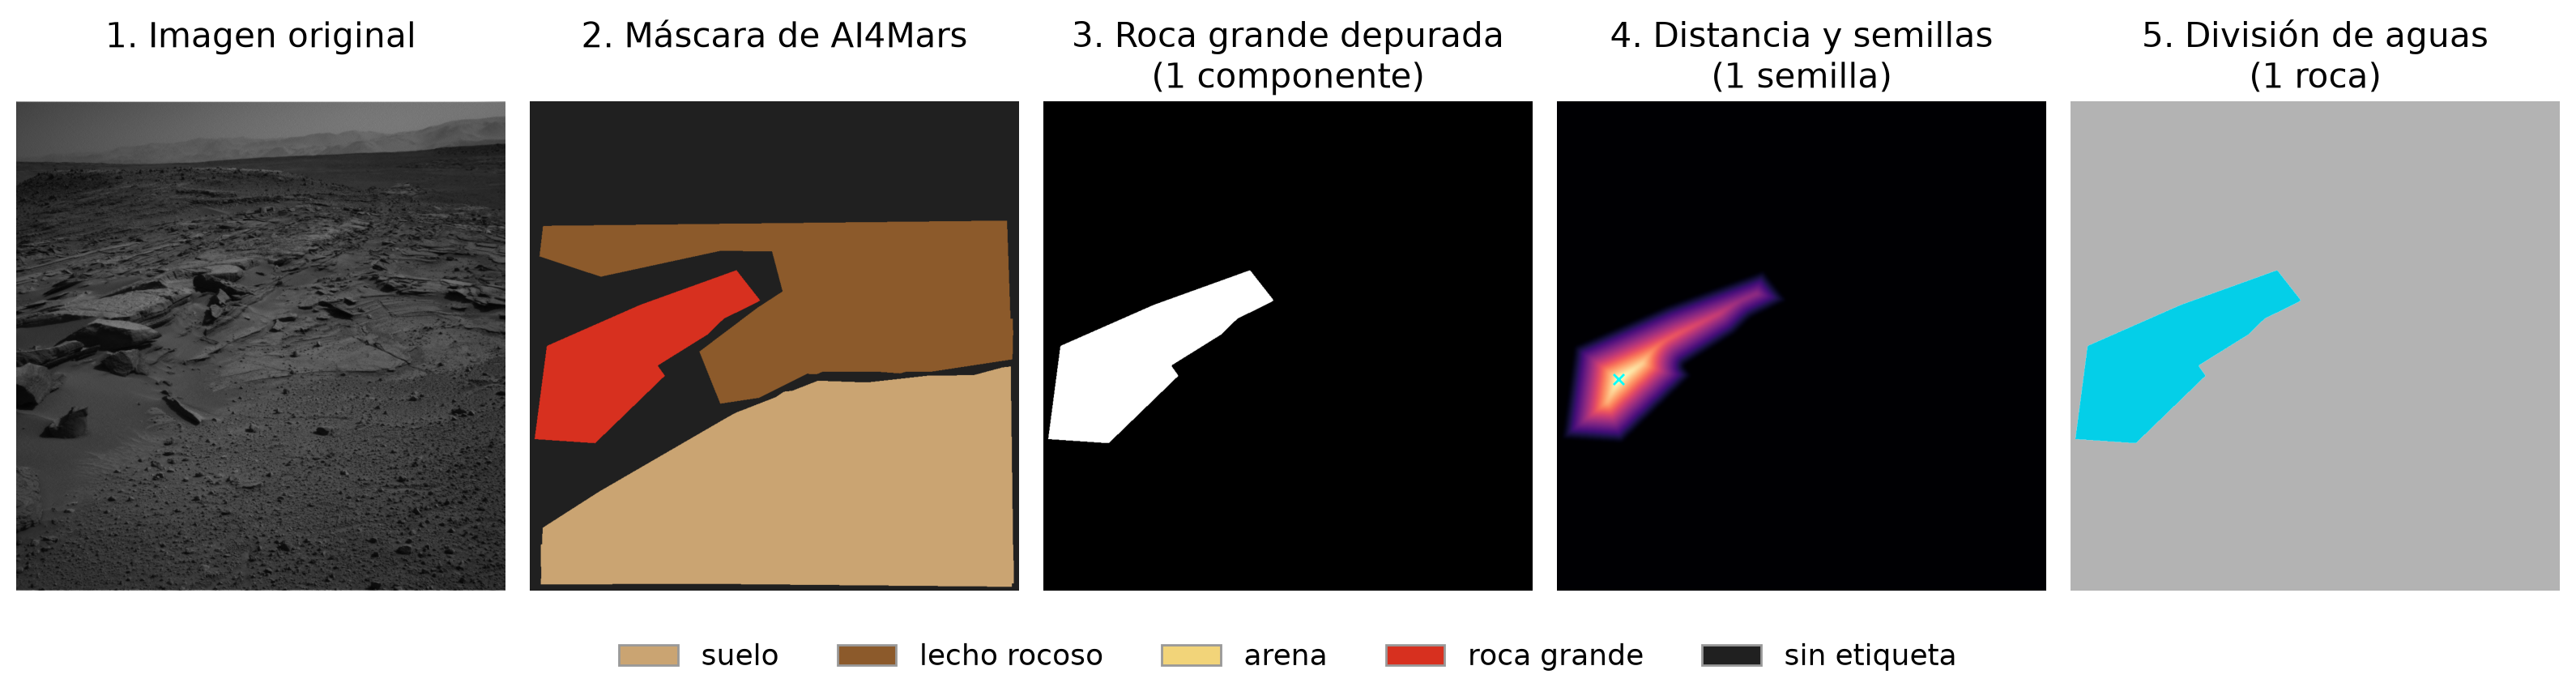
\includegraphics[width=\textwidth]{Figura_A1_procedimiento_anexo_1.png}
  \caption{Procedimiento sobre una escena con una roca aislada.}
  \label{fig:anexo1}
\end{figure}

\begin{figure}[H]
  \centering
  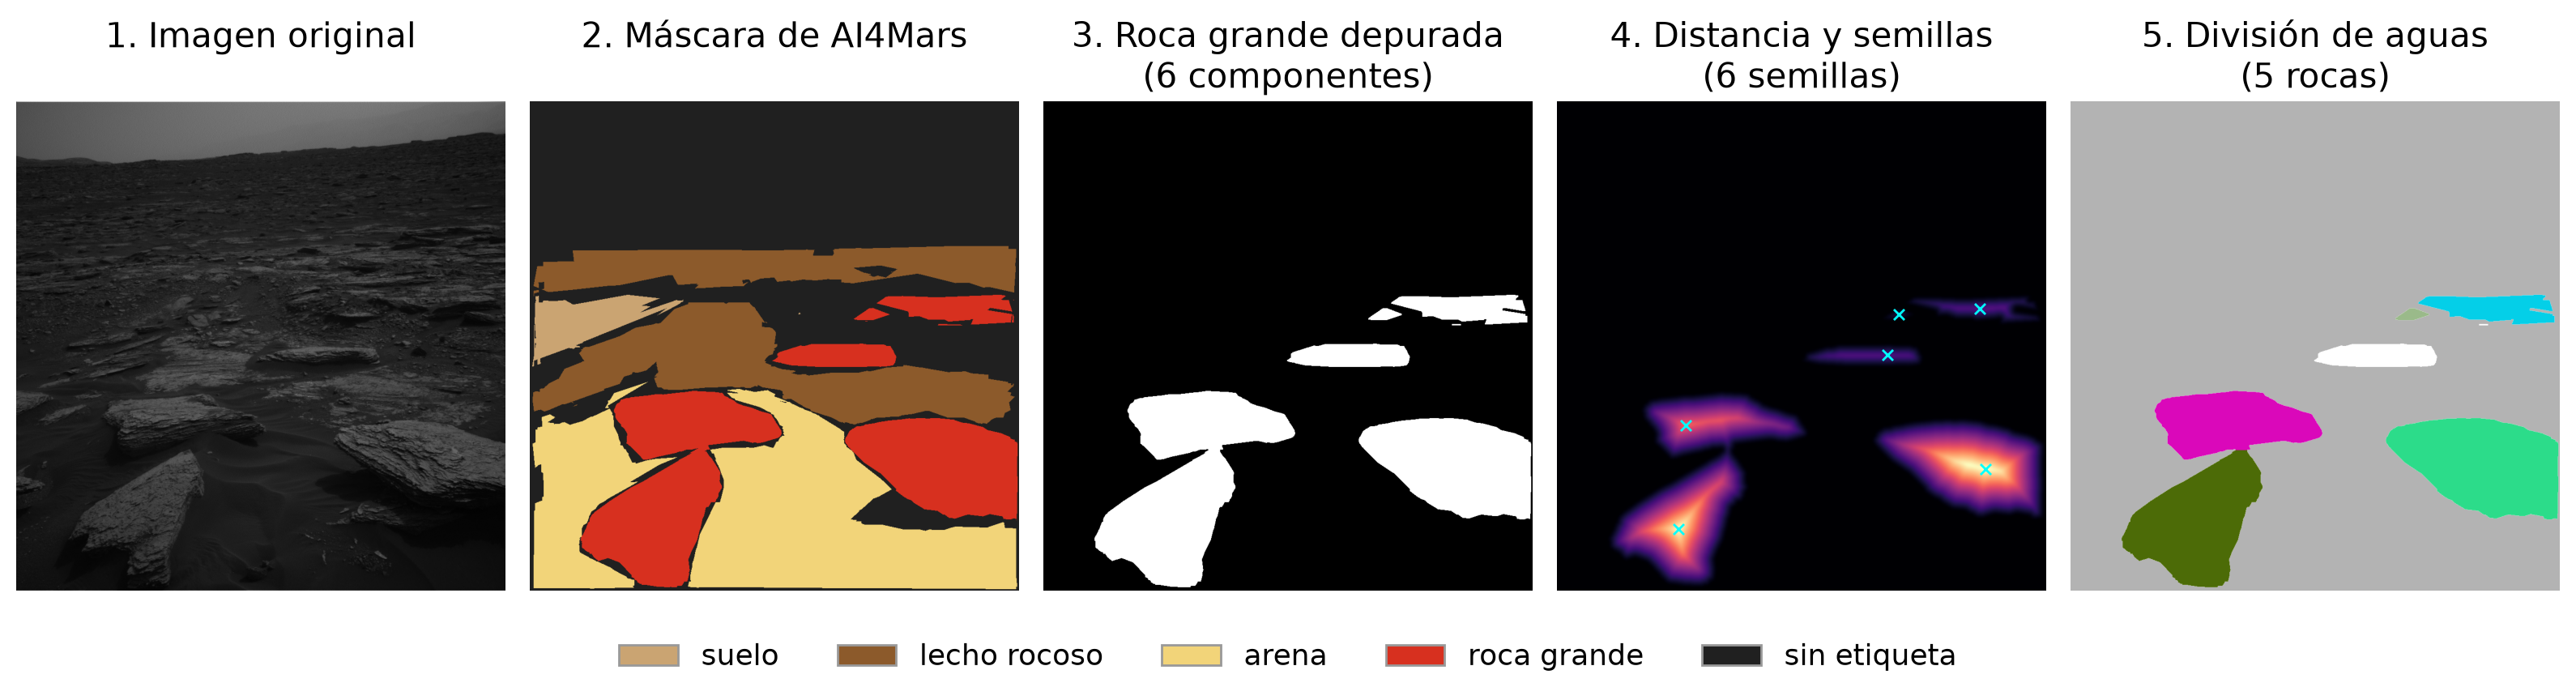
\includegraphics[width=\textwidth]{Figura_A2_procedimiento_anexo_2.png}
  \caption{Procedimiento sobre una escena con varios bloques próximos.}
  \label{fig:anexo2}
\end{figure}

\begin{figure}[H]
  \centering
  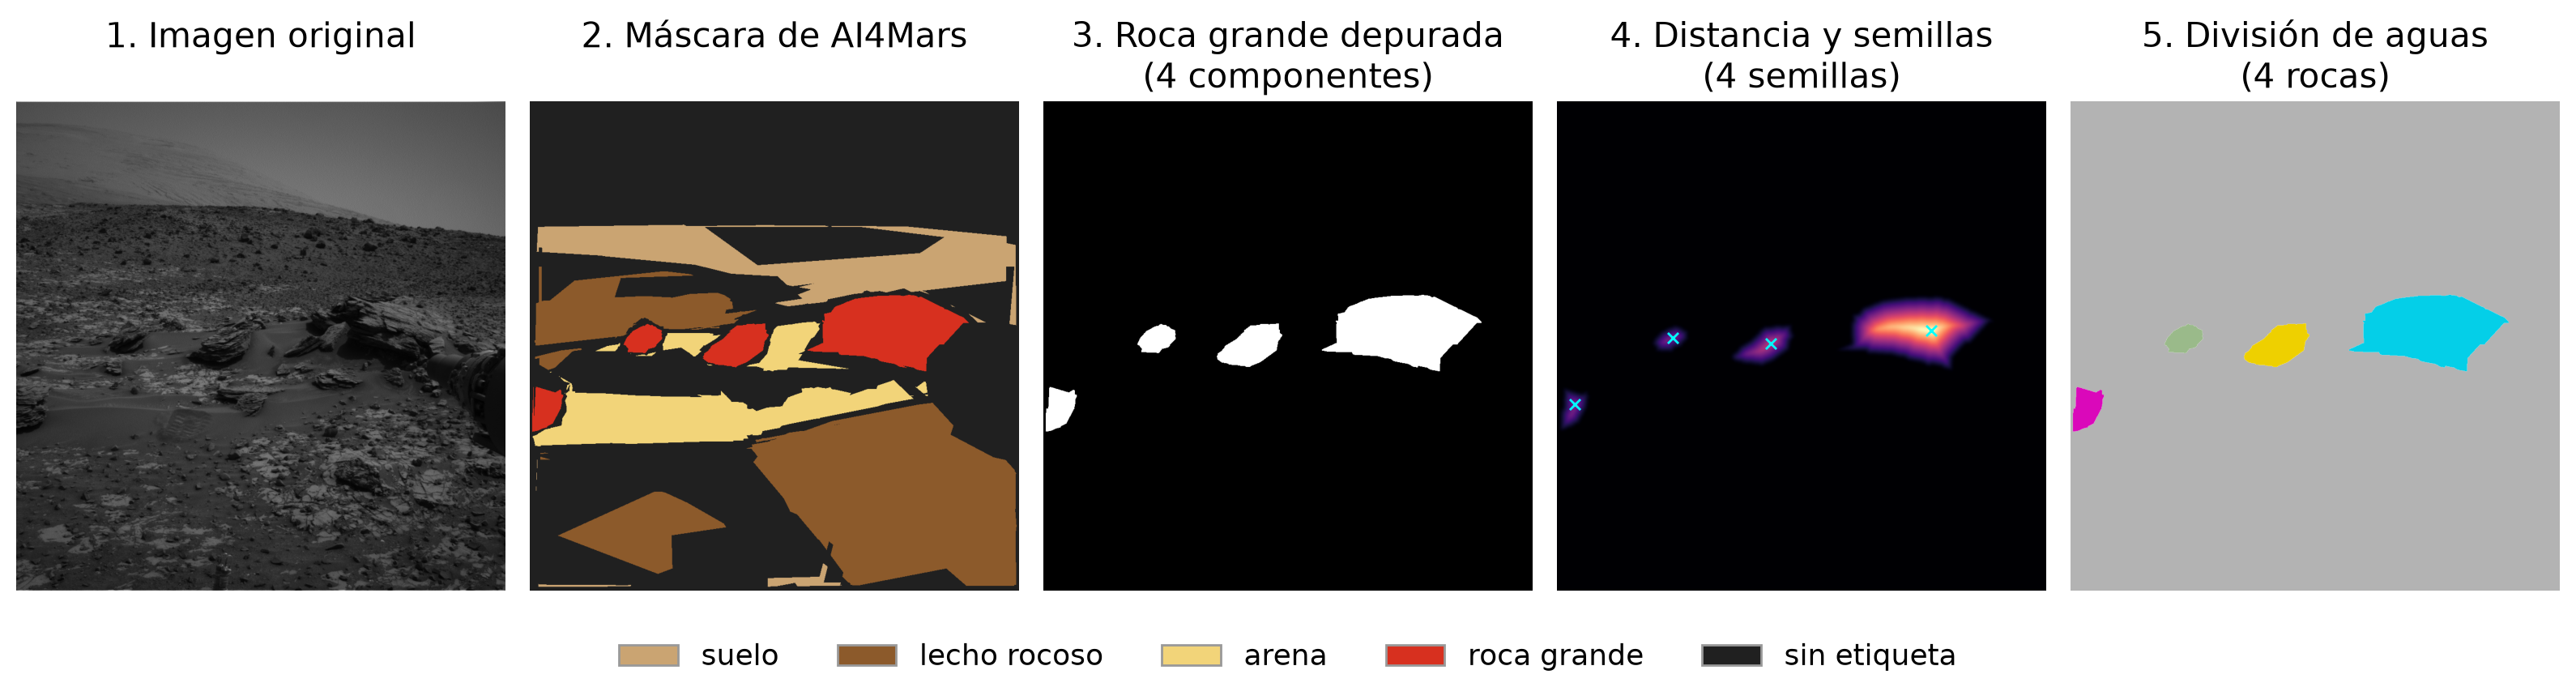
\includegraphics[width=\textwidth]{Figura_A3_procedimiento_anexo_3.png}
  \caption{Procedimiento sobre una escena de terreno mixto.}
  \label{fig:anexo3}
\end{figure}

\begin{figure}[H]
  \centering
  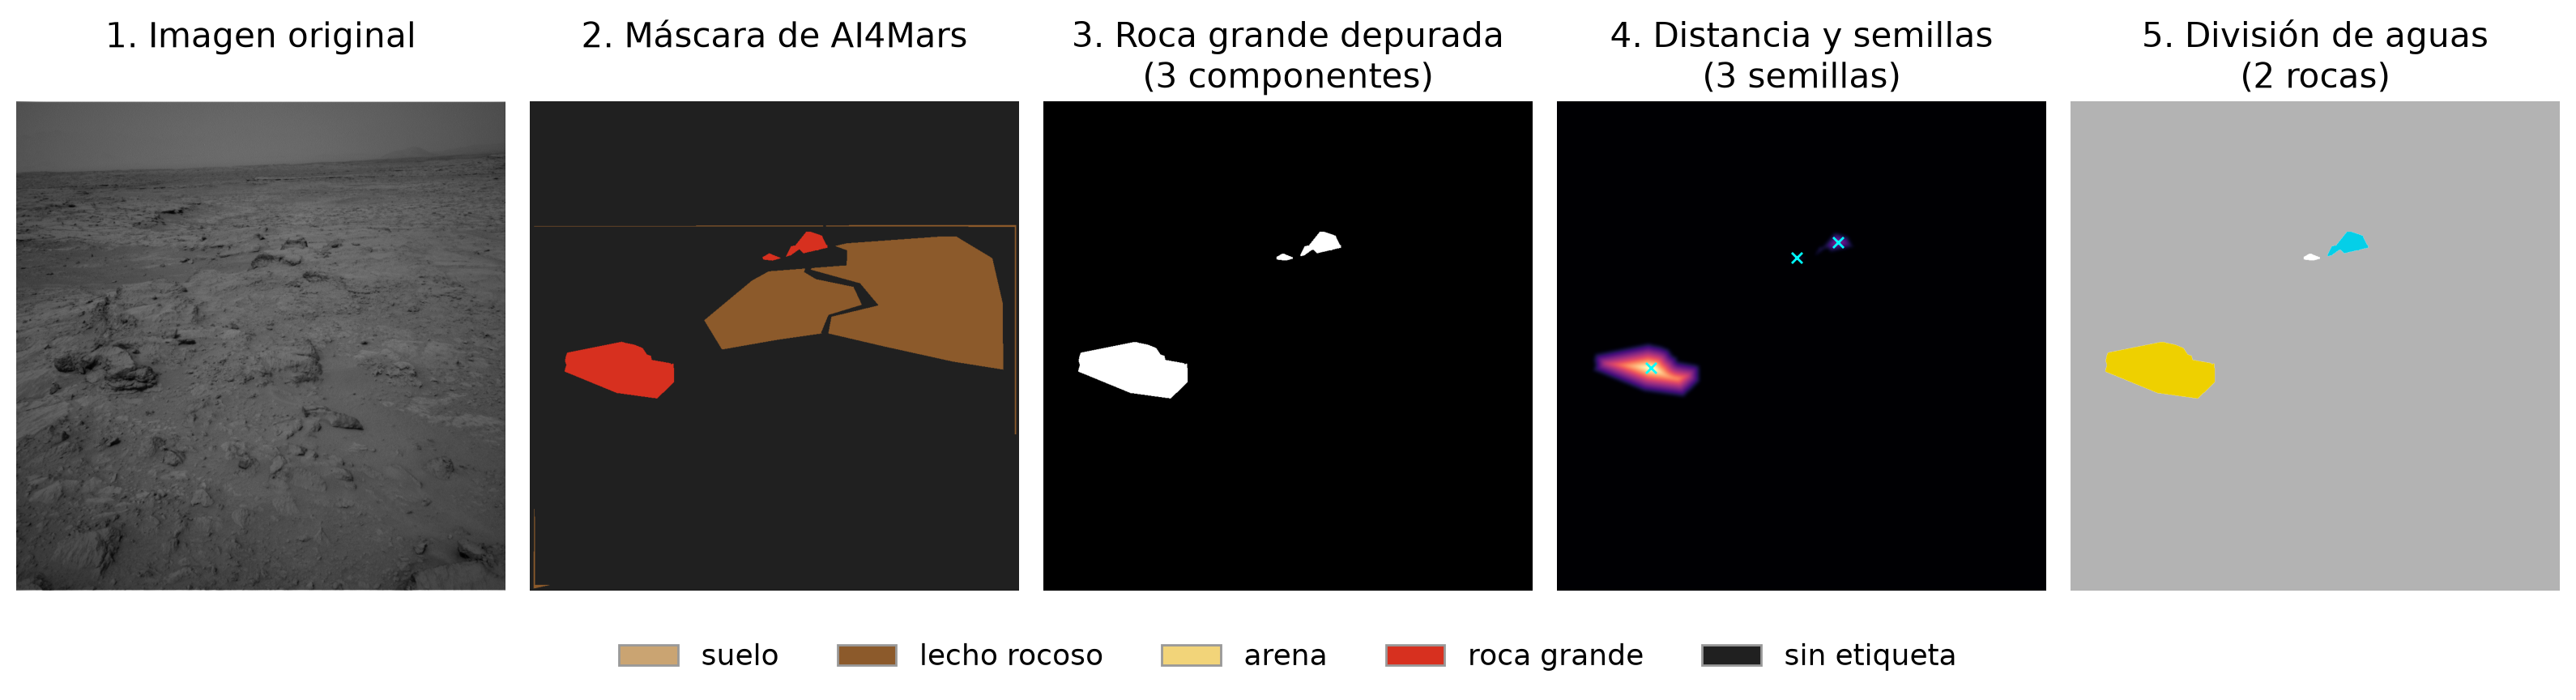
\includegraphics[width=\textwidth]{Figura_A4_procedimiento_anexo_4.png}
  \caption{Procedimiento sobre una escena dominada por afloramiento.}
  \label{fig:anexo4}
\end{figure}

\section{Modos de error descartados por los filtros}

Las dos figuras siguientes documentan los casos que el
Tabla~\ref{tab:diagnostico} atribuye a los umbrales del procedimiento, y respaldan la
afirmación de que en esas escenas los filtros aciertan.

\begin{figure}[H]
  \centering
  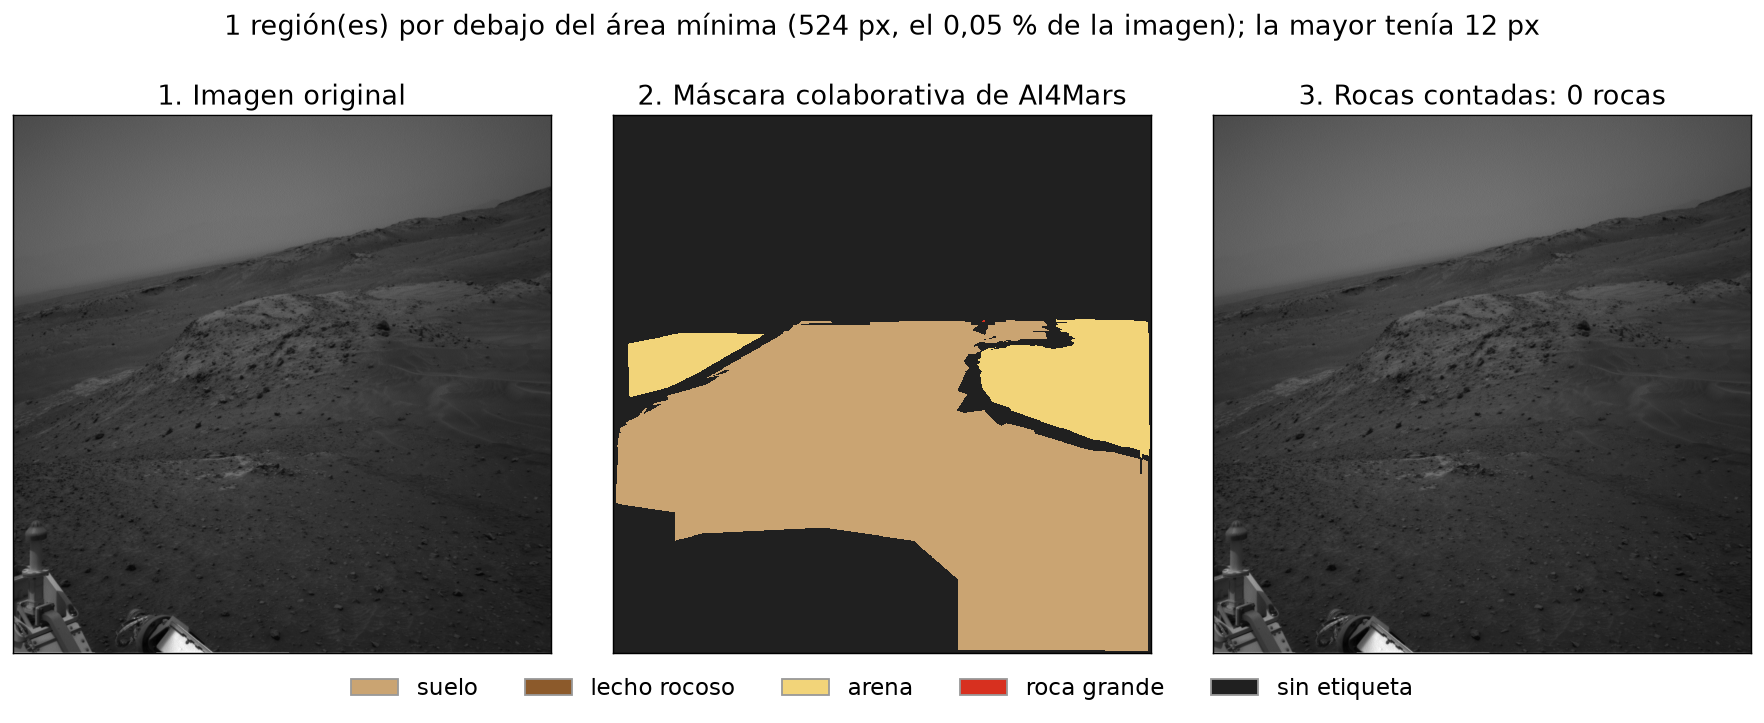
\includegraphics[width=\textwidth]{diag_bajo_umbral_area.png}
  \caption[Región por debajo del área mínima]{Escena con una única región de roca grande
    de doce píxeles, por debajo del umbral de \num{524}. El conteo devuelve cero
    correctamente.}
  \label{fig:diag-area}
\end{figure}

\begin{figure}[H]
  \centering
  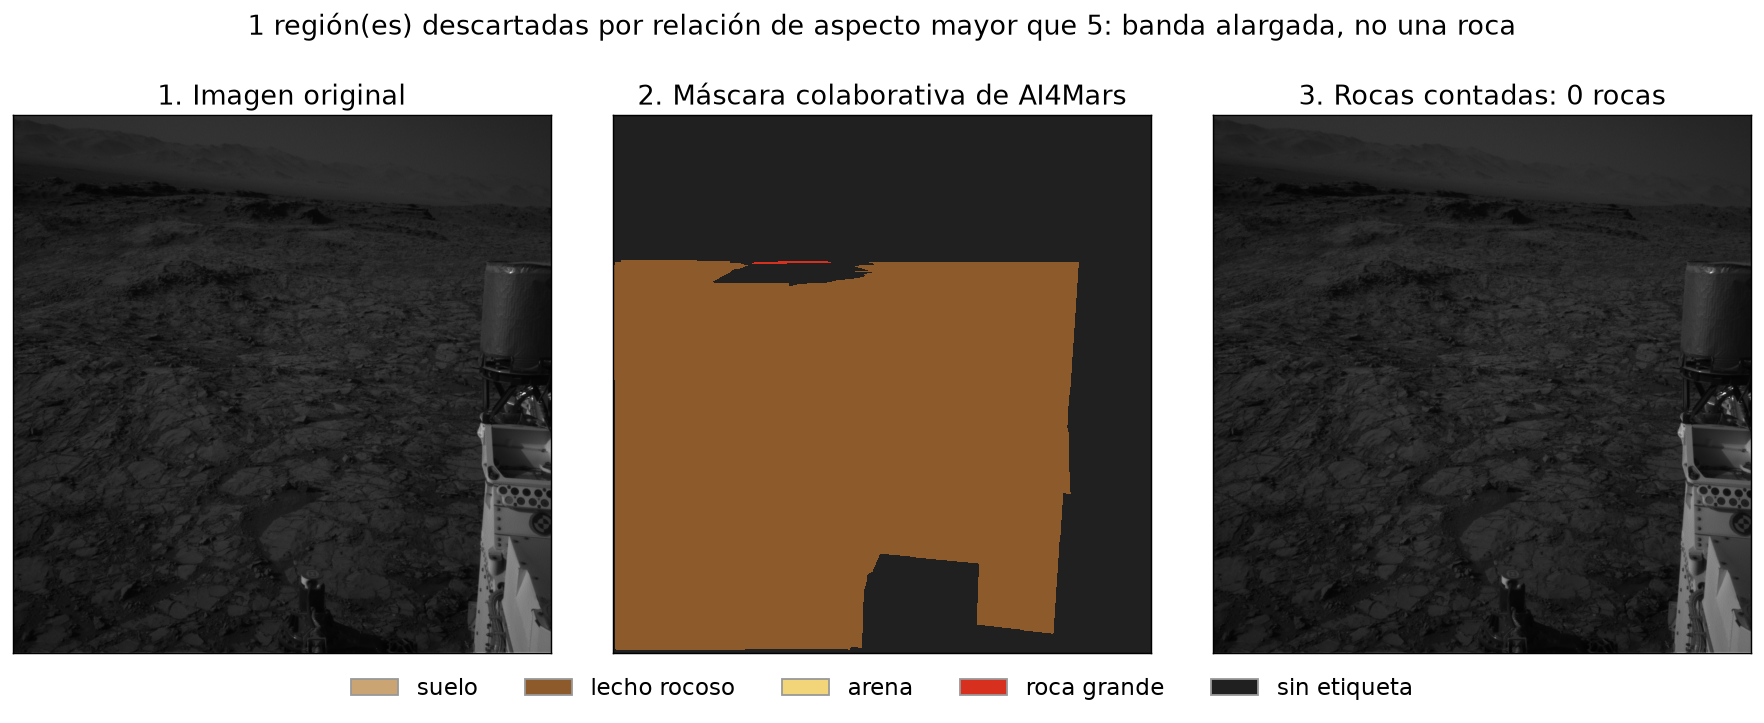
\includegraphics[width=\textwidth]{diag_filtro_aspecto.png}
  \caption[Región descartada por relación de aspecto]{Escena en la que la anotación de
    roca grande es una banda alargada trazada sobre el horizonte, descartada por relación
    de aspecto.}
  \label{fig:diag-aspecto}
\end{figure}

\begin{figure}[H]
  \centering
  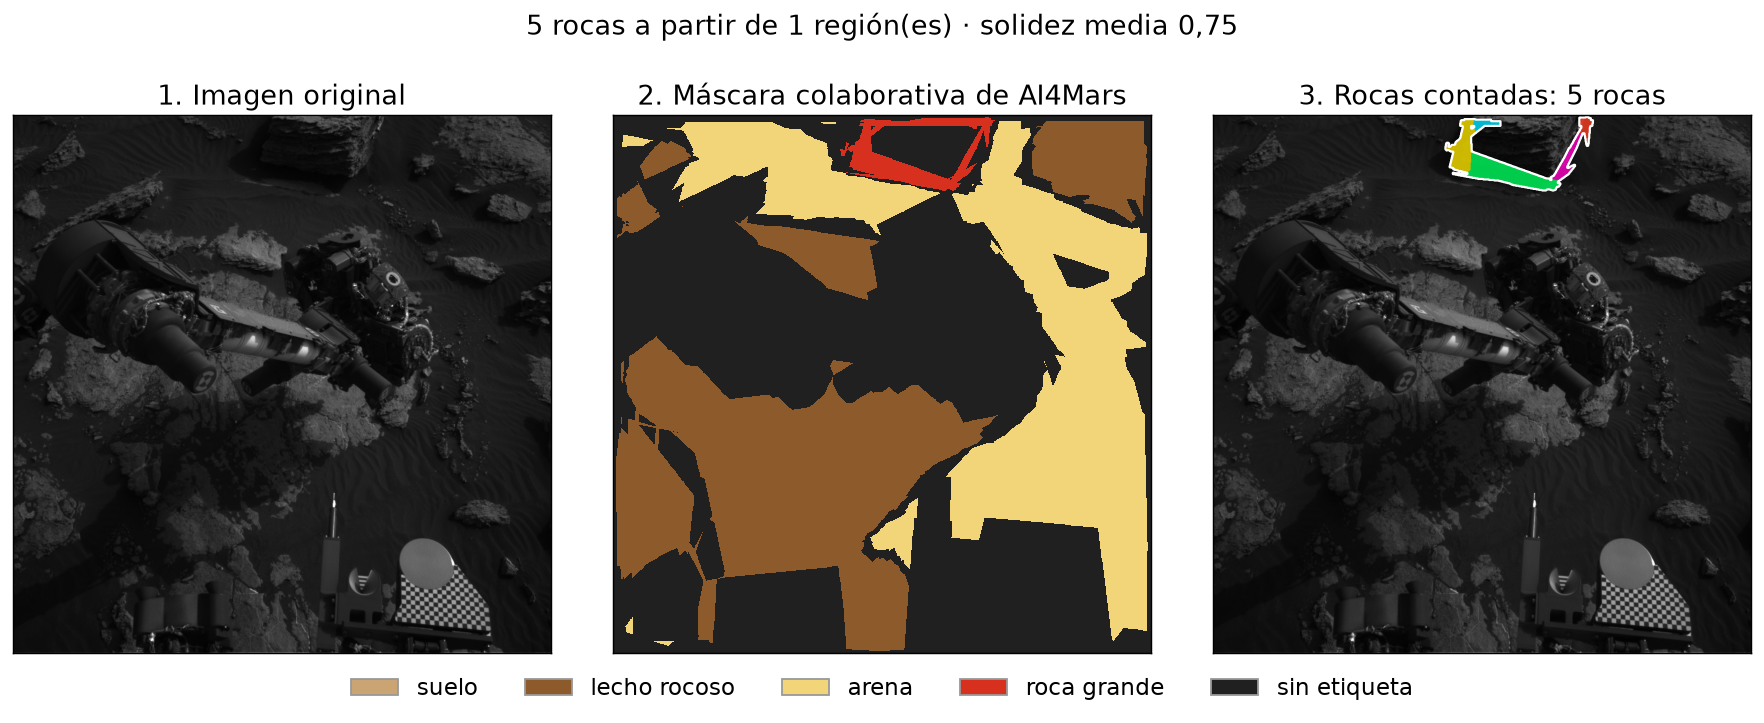
\includegraphics[width=\textwidth]{diag_sobresegmentacion.png}
  \caption[Anotación en contorno hueco]{Caso atípico de anotación trazada como contorno
    hueco. La división de aguas fragmenta el anillo resultante. Se midió que este patrón
    afecta a cerca del \SI{0.2}{\percent} de las escenas con roca grande.}
  \label{fig:diag-sobreseg}
\end{figure}

\section{Documentación técnica de la extensión aplicada}
\label{app:extension}

Esta sección documenta los componentes descritos en la
subsección~\ref{sec:extension}.

\subsection*{Capa de avisos}

Se implementa como un módulo independiente que opera sobre el archivo de resultados y le
añade cuatro columnas: las claves de los avisos activados, su número, la severidad máxima
y el nivel de riesgo resultante. Cada regla se declara como un objeto con su clave, su
título legible, su severidad, la condición —una función sobre la fila de resultados—, el
criterio en texto y su motivación. Esa estructura permite añadir, retirar o reajustar
reglas sin tocar la lógica de evaluación, y garantiza que todo umbral quede acompañado de
su justificación en el mismo lugar del código.

La evaluación no reprocesa máscaras: recorre el archivo de resultados, de modo que
recalcular los avisos sobre las \num{16064} escenas es inmediato. Las salidas son la tabla
completa con las columnas añadidas, un catálogo de las reglas con sus umbrales y un
resumen agregado por nivel y por tipo de aviso.

\subsection*{Aplicación de consulta}

Aplicación de escritorio en Python construida sobre una biblioteca de componentes gráficos
modernos, con la paleta institucional de la agencia responsable del conjunto de datos. La
ventana se organiza en una barra lateral de navegación y cuatro vistas:

\begin{description}
  \item[Resumen] Estadísticos descriptivos del subconjunto y composición del terreno.
  \item[Avisos] Distribución por nivel de riesgo y por tipo de regla, con el detalle del
    criterio que motivó cada aviso.
  \item[Explorador] Para la escena seleccionada, la imagen original, la anotación del
    terreno y las rocas detectadas por el procedimiento, en paneles contiguos.
  \item[Geología] Presencia de los rasgos de la taxonomía extendida en el conjunto de la
    misión posterior, incluidas las vetas.
\end{description}

Las figuras se generan en el momento a partir de los mismos archivos de resultados que
respaldan este documento, de modo que la aplicación no mantiene una copia propia de los
datos y cualquier reejecución del procedimiento se refleja en ella sin pasos adicionales.

\subsection*{Exploración de rasgos geológicos}

El conjunto de datos incluye, para la misión posterior a la estudiada, una taxonomía
geológica más detallada que la escala de navegación: distingue subtipos de lecho rocoso,
roca suelta, guijarros y vetas. Se recorrieron sus \num{8497} máscaras registrando la
presencia y extensión de cada rasgo. Las vetas aparecen en \num{294} escenas, el
\SI{3.5}{\percent}, de las cuales \num{150} presentan una geometría compatible con una
veta genuina —alargada y de área reducida— y \num{69} resultan dudosas.

Ese recorrido tiene un interés que excede la exploración de vetas y se recoge entre las
recomendaciones del Capítulo~\ref{cap:conclusiones}: la clase de \textit{roca suelta} de
esa taxonomía aparece en una proporción muy superior a la de \textit{roca grande} en la
escala de navegación, lo que la convierte en la vía natural para sortear el techo del
conteo documentado en la subsección~\ref{sec:diagnostico}.

\section{Recursos reproducibles}

Los recursos que respaldan el trabajo se organizan como sigue.

\begin{description}

  \item[Módulos de cálculo] Implementan la lectura de máscaras, el cálculo de cobertura,
    el conteo de rocas, los descriptores de composición y geometría, y la orquestación
    que produce una fila de resultados por imagen. Las funciones reciben arreglos y
    devuelven arreglos o números, sin efectos secundarios, y todos los umbrales se pasan
    como argumentos con valores por defecto documentados.

  \item[Guiones de ejecución] Automatizan el recorrido del subconjunto, la generación de
    las figuras del documento, el diagnóstico de los modos de error y las comparaciones
    con los métodos de aprendizaje automático.

  \item[Conjunto de resultados] Archivo tabular con los veinticuatro indicadores para las
    \num{16064} escenas, según el esquema de la Tabla~\ref{tab:esquema}.

  \item[Especificación del entorno] Archivo de definición del entorno con las
    dependencias, complementado por el registro de versiones exactas del
    Tabla~\ref{tab:versiones}.

\end{description}

El conjunto de datos AI4Mars no se distribuye con estos recursos, dado su volumen. El
código lo referencia mediante una ruta configurable, de modo que debe descargarse de la
fuente original \citep{swan2022ai4marsdata}.



% =============================================================
% REFERENCIAS
% =============================================================

\clearpage
\chapter*{Referencias}
\addcontentsline{toc}{chapter}{Referencias}
{\sloppy\printbibliography[heading=none]}

\end{document}